\documentclass[a4paper,12pt,twoside,openright]{book}

\usepackage{lmodern}
\usepackage[T2A,T1]{fontenc}
\usepackage[utf8]{inputenc}
\usepackage[portuguese,french,english]{babel}
%\usepackage[backend=biber,backref=true]{biblatex}
\usepackage[printonlyused,withpage]{acronym}
\usepackage{float}
\usepackage[hyperfootnotes=false]{hyperref}
\usepackage[chapter]{algorithm}
\usepackage{algpseudocode}
\usepackage{amsmath}
\usepackage{array}
\usepackage{caption}
\usepackage{csquotes}
\usepackage{fancyhdr}
\usepackage{lipsum}
\usepackage{listings}
\usepackage{geometry}
\usepackage{graphicx}
\usepackage{MnSymbol}
\usepackage{paralist}
\usepackage{setspace}
\usepackage{standalone}
\usepackage{subfigure}
\usepackage{tabularx}
\usepackage[disable]{todonotes}
\usepackage{minitoc}
\usepackage{styles/highlighter}
\usepackage{xcolor}

%\usepackage{tikz}
%\usepackage{styles/tikz-uml}
\usepackage[nottoc,chapter]{tocbibind}

\usepackage{textcomp}
\usepackage{epigraph}%to make quotations at start of chapter

%to force image position when doing [H]
\usepackage{float}
\usepackage{proof}
\usepackage{ stmaryrd } %for llbracket


\usepackage{bussproofs}

%%%\addbibresource{thesis.bib}


\usepackage[Lenny]{fncychap}
%styles:Sonny, Lenny, Gleen

\usepackage{pifont}


%\usepackage{vmargin}
%\special{papersize=160mm,240mm}
%\setpapersize{custom}{160mm}{240mm}
%\setmargins{1.2cm}{1.5cm}{13cm}{18.5cm}{0.6cm}{0.8cm}{0cm}{1.0cm}

% algpseudocode settings
%\algrenewcommand\alglinenumber[1]{
%    {\footnotesize#1}
%}

% prevent footnotes from breaking across pages
\interfootnotelinepenalty=10000

% redefine algorithms' frame
\makeatletter
\renewcommand\fs@ruled{%
  \def\@fs@cfont{\rmfamily}%
  \let\@fs@capt\floatc@plain%
  \def\@fs@pre{\hrule height.8pt depth0pt \kern2pt}%% or use \def\@fs@pre{} to get rid of the top rule
  \def\@fs@post{}%\def\@fs@post{\kern2pt\hrule\relax}%% or use \def\@fs@post{} to get rid of the last rule
  \def\@fs@mid{\kern2pt\hrule\kern15pt}%% or use \def\@fs@mid{} to get rid of the middle rule
  \let\@fs@iftopcapt\iffalse}
\makeatother

% define new algorithmicx blocks
\algblock{ForEach}{EndForEach}
\algnewcommand\algorithmicforeach{\textbf{for\ each}}
\algnewcommand\algorithmicforeachdo{\textbf{do}}
\algnewcommand\algorithmicendforeach{\textbf{end\ for\ each}}
\algrenewtext{ForEach}[1]{\algorithmicforeach\ #1\ \algorithmicforeachdo}
\algrenewtext{EndForEach}{\algorithmicendforeach}

\algblock{ForEachParallel}{EndForEachParallel}
\algnewcommand\algorithmicforeachparallel{\textbf{for\ each}}
\algnewcommand\algorithmicforeachparalleldo{\textbf{do\ in\ parallel}}
\algnewcommand\algorithmicendforeachparallel{\textbf{end\ for}}
\algrenewtext{ForEachParallel}[1]{\algorithmicforeachparallel\ #1\ \algorithmicforeachparalleldo}
\algrenewtext{EndForEachParallel}{\algorithmicendforeachparallel}

\algnewcommand{\CommentLeft}[1]{\State \(\triangleright\) #1}

% hyperref configuration
\hypersetup{
    colorlinks=false,
    linkcolor=red,
    urlcolor=blue,
    citecolor=green
}

% custom colors
\definecolor{darkgreen}{rgb}{0,0.6,0}

% listing configuration

\lstdefinestyle{java} {
    aboveskip=1.5em,
    basicstyle=\ttfamily\footnotesize,
    captionpos=b,
    frame=single, 
    identifierstyle=,
    language=Java,
    tabsize=4,
    numbers=left, 
    numberstyle=\scriptsize,
    xleftmargin=1.15em,     
    framexleftmargin=2em,
    escapeinside={\$}{\$},
	%commentstyle=\color{gray}
}

\lstdefinestyle{plain} {
    aboveskip=1.5em,
    basicstyle=\ttfamily\footnotesize,
    captionpos=b,
    frame=single, 
    identifierstyle=
}

\lstdefinestyle{python} {
    aboveskip=1.5em,
    language=Python,
    showstringspaces=false,
    formfeed=\newpage,
    tabsize=4,
    commentstyle=\itshape,
    captionpos=b,
    basicstyle=\ttfamily\footnotesize,
    numbers=left, 
    numberstyle=\scriptsize, 
    frame=single, 
    xleftmargin=1.15em,     
    framexleftmargin=2em,
    escapeinside={@}{@}
}

\lstdefinestyle{sparql} {
    aboveskip=1.5em,
    language=SPARQL,
    showstringspaces=false,
    formfeed=\newpage,
    tabsize=4,
    commentstyle=\itshape,
    captionpos=b,
    basicstyle=\ttfamily\footnotesize,
    numbers=left, 
    numberstyle=\scriptsize, 
    frame=single, 
    xleftmargin=1.15em,     
    framexleftmargin=2em,
    escapeinside={@}{@}
}

\lstdefinestyle{rdf} {
    aboveskip=1.5em,
    showstringspaces=false,
    formfeed=\newpage,
    tabsize=4,
    commentstyle=\itshape,
    captionpos=b,
    basicstyle=\ttfamily\footnotesize,
    numbers=left, 
    numberstyle=\scriptsize, 
    frame=single, 
    xleftmargin=1.15em,     
    framexleftmargin=2em,
    escapeinside={@}{@}
}

% tikz configuration
\usetikzlibrary{
    arrows,
    backgrounds,
    calc,
    chains,
    decorations.markings,
    decorations.pathmorphing,
    fit,
    matrix,
    patterns,
    plotmarks,
    positioning,
    shadows,
    shapes
}

% new PGF shapes

% t shape for component interfaces
\makeatletter
\pgfdeclareshape{t}{
    \inheritsavedanchors[from=rectangle]
    \inheritanchorborder[from=rectangle]
    \inheritanchor[from=rectangle]{center}
    \inheritanchor[from=rectangle]{base}
    \inheritanchor[from=rectangle]{north}
    \inheritanchor[from=rectangle]{north east}
    \inheritanchor[from=rectangle]{east}
    \inheritanchor[from=rectangle]{south east}
    \inheritanchor[from=rectangle]{south}
    \inheritanchor[from=rectangle]{south west}
    \inheritanchor[from=rectangle]{west}
    \inheritanchor[from=rectangle]{north west}
    \backgroundpath{
        % store lower right in xa/ya and upper right in xb/yb
       \southwest \pgf@xa=\pgf@x \pgf@ya=\pgf@y
       \northeast \pgf@xb=\pgf@x \pgf@yb=\pgf@y
       \pgfmathparse{(\pgf@xb-\pgf@xa)/2}
       \pgf@xc=\pgf@xa
       \advance\pgf@xc by \pgfmathresult pt
       \pgfpathmoveto{\pgfpoint{\pgf@xa}{\pgf@ya}}
       \pgfpathmoveto{\pgfpoint{\pgf@xa}{\pgf@yb}}
       \pgfpathlineto{\pgfpoint{\pgf@xb}{\pgf@yb}}
       \pgfpathmoveto{\pgfpoint{\pgf@xc}{\pgf@yb}}
       \pgfpathlineto{\pgfpoint{\pgf@xc}{\pgf@ya}}
   }
}
\makeatother

\captionsetup[algorithm]{
    justification=centering,labelfont=normalfont,labelsep=endash
}

% increase line spacing
\onehalfspacing

% rename the default name of the table of contents
% from 'Contents' to 'Table of Content'
\addto\captionsenglish{
    \renewcommand\contentsname{Table of Contents\vspace{-5pt}}
}

% define abstract environment since it is not available 
% with book document class
\newenvironment{abstract}{
    \null\vfill
    \begin{center}
        \bfseries\abstractname
    \end{center}
}{
    \vfill\null\clearpage
}

% custom minitoc command to have extra space after 
% the mini table of content
\newcommand{\cminitoc}{
    \minitoc
    \vspace{1em}
}

% Group list of listings by chapter
\makeatletter
\let\my@chapter\@chapter
\renewcommand*{\@chapter}{%
  \addtocontents{lol}{\protect\addvspace{7pt}}%
  \my@chapter}
\makeatother

% reconfigure list of listings commands
\renewcommand{\lstlistlistingname}{List of Listings}

\renewcommand{\lstlistoflistings}{
    \begingroup
    \tocfile{\lstlistlistingname}{lol}
    \endgroup
    \mtcaddchapter
}

% tabular helper
\newcommand*{\tabbox}[2][t]{
        \vspace{0pt
    }\parbox[#1][3.7\baselineskip]{1.35cm}{\strut#2\strut}
}

% bibliography, backref text
%\DefineBibliographyStrings{english}{
 %   backrefpage = {cited on p.},
 %   backrefpages= {cited on pp.},
%}

\newcolumntype{Y}{>{\centering\arraybackslash}X}

\definecolor{orange}{rgb}{1,0.5,0}
\definecolor{redcomment}{rgb}{0.5,0,0}


\lstdefinelanguage{Coqfix}{  
  sensitive=true,
  morecomment=[l]{//},      %single line comment 
  morecomment=[s]{(*}{*)}, %normal comment
 morecomment=[n]{(*}{*)},  %nested comment
  morestring=[b]",    
  basicstyle=\footnotesize,           % the size of the fonts that are used for the code
  numbers=left,                   % where to put the line-numbers
  numberstyle=\tiny\color{black},  % the style that is used for the line-numbers
  stepnumber=1,                   % the step between two line-numbers. If it's 1, each line 
                                  % will be numbered
  numbersep=5pt,                  % how far the line-numbers are from the code
  backgroundcolor=\color{white},      % choose the background color. You must add \usepackage{color}
  showspaces=false,               % show spaces adding particular underscores
  showstringspaces=false,         % underline spaces within strings
  showtabs=false,                 % show tabs within strings adding particular underscores
  %frame=single,                   % adds a frame around the code
  rulecolor=\color{black},        % if not set, the frame-color may be changed on line-breaks within not-black text (e.g. commens (green here))
  tabsize=2,                      % sets default tabsize to 2 spaces
  captionpos=b,                   % sets the caption-position to bottom
  breaklines=true,                % sets automatic line breaking
  breakatwhitespace=false,        % sets if automatic breaks should only happen at whitespace
  %title=\lstname,                   % show the filename of files included with \lstinputlisting;
                                  % also try caption instead of title
  keywordstyle=\color{red},          % keyword style
  keywordstyle=[2]\color{blue},          % keyword style
  commentstyle=\color{redcomment},       % comment style
  stringstyle=\color{orange},         % string literal style
  escapeinside={\%*}{*)},            % if you want to add a comment within your code
  morekeywords={Inductive, Definition, Function, Fixpoint, Lemma, Theorem, Eval, Parameter},      % if you want to add more keywords to the set
 morekeywords={[2] Prop, Type, with, match, end, Proof, Qed, forall, Notation, if, then, else, Case, compute, let, in, return, Defined, as, fix}   % if you want to add more keywords to the set
}

\lstdefinelanguage{Coq}{  
  sensitive=true,
  morecomment=[l]{//},      %single line comment 
  morecomment=[s]{(*}{*)}, %normal comment
 morecomment=[n]{(*}{*)},  %nested comment
  morestring=[b]",    
  basicstyle=\footnotesize,           % the size of the fonts that are used for the code
  numbers=left,                   % where to put the line-numbers
  numberstyle=\tiny\color{black},  % the style that is used for the line-numbers
  stepnumber=1,                   % the step between two line-numbers. If it's 1, each line 
                                  % will be numbered
  numbersep=5pt,                  % how far the line-numbers are from the code
  backgroundcolor=\color{white},      % choose the background color. You must add \usepackage{color}
  showspaces=false,               % show spaces adding particular underscores
  showstringspaces=false,         % underline spaces within strings
  showtabs=false,                 % show tabs within strings adding particular underscores
  %frame=single,                   % adds a frame around the code
  rulecolor=\color{black},        % if not set, the frame-color may be changed on line-breaks within not-black text (e.g. commens (green here))
  tabsize=2,                      % sets default tabsize to 2 spaces
  captionpos=b,                   % sets the caption-position to bottom
  breaklines=true,                % sets automatic line breaking
  breakatwhitespace=false,        % sets if automatic breaks should only happen at whitespace
  %title=\lstname,                   % show the filename of files included with \lstinputlisting;
                                  % also try caption instead of title
  keywordstyle=\color{red},          % keyword style
  keywordstyle=[2]\color{blue},          % keyword style
  commentstyle=\color{redcomment},       % comment style
  stringstyle=\color{orange},         % string literal style
  escapeinside={\%*}{*)},            % if you want to add a comment within your code
  morekeywords={Record, CoInductive, Inductive, Definition, Function, CoFixpoint, Fixpoint, Lemma, Theorem, Eval, Parameter},      % if you want to add more keywords to the set
 morekeywords={[2] Prop, Type, with, match, end, Proof, Qed, forall, Notation, if, then, else, Case, compute, let, in, return, Defined, as, exists}   % if you want to add more keywords to the set
}


\lstdefinelanguage{OCaml}{  
  sensitive=true,
  morecomment=[l]{//},      %single line comment 
  morecomment=[s]{(*}{*)}, %normal comment
 morecomment=[n]{(*}{*)},  %nested comment
  morestring=[b]",    
  basicstyle=\footnotesize,           % the size of the fonts that are used for the code
  numbers=left,                   % where to put the line-numbers
  numberstyle=\tiny\color{black},  % the style that is used for the line-numbers
  stepnumber=1,                   % the step between two line-numbers. If it's 1, each line 
                                  % will be numbered
  numbersep=5pt,                  % how far the line-numbers are from the code
  backgroundcolor=\color{white},      % choose the background color. You must add \usepackage{color}
  showspaces=false,               % show spaces adding particular underscores
  showstringspaces=false,         % underline spaces within strings
  showtabs=false,                 % show tabs within strings adding particular underscores
  %frame=single,                   % adds a frame around the code
  rulecolor=\color{black},        % if not set, the frame-color may be changed on line-breaks within not-black text (e.g. commens (green here))
  tabsize=2,                      % sets default tabsize to 2 spaces
  captionpos=b,                   % sets the caption-position to bottom
  breaklines=true,                % sets automatic line breaking
  breakatwhitespace=false,        % sets if automatic breaks should only happen at whitespace
  %title=\lstname,                   % show the filename of files included with \lstinputlisting;
                                  % also try caption instead of title
  keywordstyle=\color{red},          % keyword style
  keywordstyle=[2]\color{blue},          % keyword style
  commentstyle=\color{redcomment},       % comment style
  stringstyle=\color{black},         % string literal style
  escapeinside={\%*}{*)},            % if you want to add a comment within your code
  morekeywords={ int, float, string, Obj},               % if you want to add more keywords to the set
 morekeywords={[2] fun, let, function, if, then, else, match, with, in}               % if you want to add more keywords to the set
}


\lstdefinelanguage{MyXML}{  
  sensitive=true,
  %morecomment=[l]{<!--},      %single line comment 
  morecomment=[s]{<!--}{-->}, %normal comment
 morecomment=[n]{<!--}{-->},  %nested comment
  morestring=[b]",    
  basicstyle=\footnotesize,           % the size of the fonts that are used for the code
  numbers=left,                   % where to put the line-numbers
  numberstyle=\tiny\color{black},  % the style that is used for the line-numbers
  stepnumber=1,                   % the step between two line-numbers. If it's 1, each line 
                                  % will be numbered
  numbersep=5pt,                  % how far the line-numbers are from the code
  backgroundcolor=\color{white},      % choose the background color. You must add \usepackage{color}
  showspaces=false,               % show spaces adding particular underscores
  showstringspaces=false,         % underline spaces within strings
  showtabs=false,                 % show tabs within strings adding particular underscores
  %frame=single,                   % adds a frame around the code
  rulecolor=\color{black},        % if not set, the frame-color may be changed on line-breaks within not-black text (e.g. commens (green here))
  tabsize=2,                      % sets default tabsize to 2 spaces
  captionpos=b,                   % sets the caption-position to bottom
  breaklines=true,                % sets automatic line breaking
  breakatwhitespace=false,        % sets if automatic breaks should only happen at whitespace
  %title=\lstname,                   % show the filename of files included with \lstinputlisting;
                                  % also try caption instead of title
  keywordstyle=\color{red},          % keyword style
  keywordstyle=[2]\color{blue},          % keyword style
  keywordstyle=[3]\bfseries,
  keywordstyle=[4]\color{darkgreen},
  commentstyle=\color{redcomment},       % comment style
  stringstyle=\color{orange},         % string literal style
  escapeinside={\%*}{*)},            % if you want to add a comment within your code
  morekeywords={DOCTYPE, PUBLIC},            
 morekeywords={[2] definition},       
 morekeywords={[3] interface, content, controller},
 morekeywords={[4] desc, class, signature, name, role}
}

\lstdefinelanguage{Fiacre}{  
  sensitive=true,
  morecomment=[l]{//},      %single line comment 
  morecomment=[s]{/*}{*/}, %normal comment
 morecomment=[n]{/*}{*/},  %nested comment
  morestring=[b]",    
  basicstyle=\footnotesize,           % the size of the fonts that are used for the code
  numbers=left,                   % where to put the line-numbers
  numberstyle=\tiny\color{black},  % the style that is used for the line-numbers
  stepnumber=1,                   % the step between two line-numbers. If it's 1, each line 
                                  % will be numbered
  numbersep=5pt,                  % how far the line-numbers are from the code
  backgroundcolor=\color{white},      % choose the background color. You must add \usepackage{color}
  showspaces=false,               % show spaces adding particular underscores
  showstringspaces=false,         % underline spaces within strings
  showtabs=false,                 % show tabs within strings adding particular underscores
  %frame=single,                   % adds a frame around the code
  rulecolor=\color{black},        % if not set, the frame-color may be changed on line-breaks within not-black text (e.g. commens (green here))
  tabsize=2,                      % sets default tabsize to 2 spaces
  captionpos=b,                   % sets the caption-position to bottom
  breaklines=true,                % sets automatic line breaking
  breakatwhitespace=false,        % sets if automatic breaks should only happen at whitespace
  %title=\lstname,                   % show the filename of files included with \lstinputlisting;
                                  % also try caption instead of title
  keywordstyle=\color{red},          % keyword style
  keywordstyle=[2]\color{blue},          % keyword style
  keywordstyle=[3]\bfseries,
  keywordstyle=[4]\color{darkgreen},
  commentstyle=\color{redcomment},       % comment style
  stringstyle=\color{orange},         % string literal style
  escapeinside={\%*}{*)},            % if you want to add a comment within your code
  morekeywords={type, process, union, is, record, const, component, par},            
 morekeywords={[2] from, if, to, end, select},       
 morekeywords={[3] var, states},
 morekeywords={[4] in, out}
}

\lstdefinelanguage{Fiacretypes}{  
  sensitive=true,
  morecomment=[l]{//},      %single line comment 
  morecomment=[s]{/*}{*/}, %normal comment
 morecomment=[n]{/*}{*/},  %nested comment
  morestring=[b]",    
  basicstyle=\footnotesize,           % the size of the fonts that are used for the code
  numbers=left,                   % where to put the line-numbers
  numberstyle=\tiny\color{black},  % the style that is used for the line-numbers
  stepnumber=1,                   % the step between two line-numbers. If it's 1, each line 
                                  % will be numbered
  numbersep=5pt,                  % how far the line-numbers are from the code
  backgroundcolor=\color{white},      % choose the background color. You must add \usepackage{color}
  showspaces=false,               % show spaces adding particular underscores
  showstringspaces=false,         % underline spaces within strings
  showtabs=false,                 % show tabs within strings adding particular underscores
  %frame=single,                   % adds a frame around the code
  rulecolor=\color{black},        % if not set, the frame-color may be changed on line-breaks within not-black text (e.g. commens (green here))
  tabsize=2,                      % sets default tabsize to 2 spaces
  captionpos=b,                   % sets the caption-position to bottom
  breaklines=true,                % sets automatic line breaking
  breakatwhitespace=false,        % sets if automatic breaks should only happen at whitespace
  %title=\lstname,                   % show the filename of files included with \lstinputlisting;
                                  % also try caption instead of title
  keywordstyle=\color{red},          % keyword style
  keywordstyle=[2]\color{blue},          % keyword style
  keywordstyle=[3]\bfseries,
  keywordstyle=[4]\color{darkgreen},
  commentstyle=\color{redcomment},       % comment style
  stringstyle=\color{orange},         % string literal style
  escapeinside={\%*}{*)},            % if you want to add a comment within your code
  morekeywords={type, process, union, is, record, const, component, par, end},            
 morekeywords={[2] from, if, to, select},       
 morekeywords={[3] var, states},
 morekeywords={[4] in, out}
}


\newcommand{\thehm}{\textsc{The HyperManager}}
\newcommand{\pnets}{\textit{pNets}}
\newcommand{\spinnaker}{\textsf{Spinnaker}}
\newcommand{\gcm}{\ac{GCM}}
\newcommand{\adl}{\ac{ADL}}

\newcommand{\chapbreak}{\begin{center}\ding{64}\ding{64}\ding{64}\end{center}}

\newcommand{\red}[1]{\textcolor{red}{#1}}
\newcommand{\blue}[1]{\textcolor{blue}{#1}}
\newcommand{\env}{\Gamma}


%\newcommand{\origunderscore}{}
%\let\origunderscore\_
%\renewcommand{\_}{\allowbreak\origunderscore}

\usepackage{underscore}

\usepackage{amsthm}%for \qed
%\newcommand{\proof}{\vspace*{-1ex} \noindent {\bf Proof: }}
%\newcommand{\proofsketch}{\vspace*{-1ex} \noindent {\bf Proof Sketch: }}

%% TODO: reset acronym counter


\newtheorem{definition}{Definition}[section]
\newtheorem{property}{Property}[section]


\definecolor{redlemma}{rgb}{0.9,0,0}
\newtheorem{lemma}{\textcolor{redlemma}{Lemma}}[section]
\newtheorem{theorem}{\textcolor{redlemma}{Theorem}}[section]

\newenvironment{changemargin}[2]{% 
\begin{list}{}{% 
	 \setlength{\topsep}{0pt}% 
    \setlength{\leftmargin}{#1}% 
    \setlength{\rightmargin}{#2}% 
    \setlength{\listparindent}{\parindent}% 
    \setlength{\itemindent}{\parindent}% 
    \setlength{\parsep}{\parskip}% 
}% 
\item[]}{\end{list}} 


\begin{document}
    \dominitoc

    % commands to use are \todo{...} and \missingfigure{...}
    \listoftodos

    \frontmatter
    \newgeometry{top=1in,bottom=1in,right=1in,left=1in}

\begin{titlepage}
   \vspace*{-1.44cm}
   \begin{center}
       {\sffamily\MakeUppercase{Universit\'e de Nice-Sophia Antipolis}}\\
       \vspace*{3mm}
       \bsc{
            École Doctorale STIC\\[0.5ex]
            \small{Sciences et Technologies de l'Information et de la Communication}
        }\\
        \vspace{1cm}
        {\Large\bfseries THÈSE}\\
        \vspace*{5mm} 
        \textit{pour l'obtention du titre de}\\ 
        \vspace*{5mm}
        {\Large\bfseries Docteur en Sciences}\\
        \vspace*{5mm} 
        {\bfseries Mention Informatique}\\
        \vskip 5mm
        \textit{présentée et soutenue par}\\
        \vskip 5mm
        {\Large\bfseries Nuno \bsc{Gaspar}}
        \vskip 10mm
        {\fontsize{22}{1\baselineskip}\selectfont\textbf{Mechanized support for the formal\\[1mm]
        specification, verification and deployment\\[1mm]
        of component-based applications }}
        \vskip 10mm 
        \textit{Thèse dirigée par Eric \bsc{Madelaine}\\et co-encadrée par  Ludovic \bsc{Henrio}}\\
        \vskip 5mm
        %\textit{au sein de l'équipe SCALE, équipe commune de l'INRIA Sophia Antipolis,\\ du CNRS et du laboratoire I3S}
        \vskip 5mm
        \textit{Soutenue le X D\'ecembre 2014}
        \vfill
        \vspace*{7mm}
		\begin{center}
			\textbf{Jury}
		\end{center}
        \begin{tabular}{rll}
            \textit{Rapporteurs}           & Xyz \bsc{Xyz}  & Affil Xyz\\[2mm]
                                           & Xyz \bsc{Xyz}  & Affil Xyz\\[2mm]
			\textit{Examinateurs}          & Xyz \bsc{Xyz}  & Affil Xyz \\[2mm]
			                               & Xyz \bsc{Xyz}    & Affil Xyz \\[2mm]
            \textit{Directeur de thèse}    & Eric \bsc{Madelaine}  & Université de Nice-Sophia Antipolis \\[2mm]
            \textit{Co-encadrant de thèse} & Ludovic \bsc{Henrio}     & Université de Nice-Sophia Antipolis \\[2mm]
        \end{tabular}
    \end{center}
\end{titlepage}

\restoregeometry
\cleardoublepage

    \begin{flushright}
	\null\vspace{\stretch{1}}
	\textit{Future me, be happy, its done.}
	\vspace{\stretch{2}}\null
\end{flushright}

\cleardoublepage

    %\selectlanguage{french}
%\begin{abstract}

%GCM

%\end{abstract}

\chapter*{\centering R\'esum\'e}

Cette thèse appartient au domaine des méthodes formelles. 
Que ce soit par le biais d'approches automatiques ou interactives, l'objectif des méthodes formelles 
est d'accroître la confiance que l'on peut placer sur les propriétés d'un système. 
Dans cette thèse, nous concentrons 
leur application sur une méthodologie spécifique 
pour le développement de logiciels: l'ingénierie à base de composants. 


Parmi tous les paradigmes de programmation, de l'ingénierie à base de composants se présente comme une 
des approches les plus suivies pour le développement de logiciels dans le monde réel. Elle met l'accent 
sur une séparation nette des préoccupations, attrayant ainsi pour des fins industriels 
et de recherche. En outre, elle permet des reconfigurations structurelle 
de l'architecture des applications. L'avantage de la modification de l'architecture du logiciel 
vient de la nécessité de faire face à la multitude de situations 
qui peuvent survenir dans un système potentiellement massivement distribué et hétérogène. 
À cette fin, le \textit{Grid Component Model} (GCM) suis cette approche en fournissant touts  
les moyens pour définir, composer, et dynamiquement reconfigurer les applications distribuées 
à base de composants. 


Dans cette thèse, nous abordons la spécification formelle, la vérification et le déploiement
 d'applications GCM reconfigurables et distribués. Notre première contribution est un cas d'étude 
industriel 
 sur la spécification comportementale et la vérification d'une application distribuée et 
 reconfigurable: \textsc{The HyperManager}. 
Cela favorise l'utilisation des méthodes formelles dans un contexte industriel, 
     mais met également en évidence la nécessité d'approches alternatives et/ou complémentaires 
afin de mieux répondre à ces entreprises. 

Notre deuxième contribution est une plate-forme, élaboré avec l'assistant de preuve Coq, 
pour le raisonnement sur ​​les architectures logicielles: \textsc {Mefresa} . Cela comprend 
la mécanisation de la spécification du GCM, et les moyens pour 
raisonner sur les architectures reconfigurables GCM. En outre, nous adressons 
les aspects comportementaux en formalisant une sémantique basée sur les traces d'exécution de 
systèmes de transitions synchronisées. 
Dans l'ensemble, elle fournit les premiers pas vers une plate-forme complète pour la spécification 
et la vérification des caractéristiques structurelle et comportementale. 

Enfin, notre troisième contribution est un nouveau langage de description d'architecture (ADL): 
\textsc{Painless}. En outre, nous discutons son intégration avec ProActive --- 
un intergiciel Java pour la programmation concurrente et distribuée, 
et l'implantation référence du GCM. 
\textsc{Painless} permet de spécifier des architectures de GCM paramétrées, avec 
leurs reconfigurations structurelle, dans un langage déclaratif. Conformité 
avec la spécification de GCM est évaluée par le code fonctionnel certifié extrait de 
\textsc{Mefresa} . Ceci permet le déploiement et
reconfigurations sûre des applications du GCM.





%\selectlanguage{english}
%\begin{abstract}

\chapter*{\centering Abstract}
\addcontentsline{toc}{chapter}{Abstract}

		This thesis belongs to the domain of formal methods.  
	Let it be by means of automatic or interactive approaches, the goal of formal methods
	is to increase the confidence one can place on a system's properties.
	In this thesis, we focus 
		their application on a specific methodology
	for the development of software: component-based engineering.


		Among all programming paradigms, component-based engineering stands as one
	of the most followed approaches for real world software development. Its emphasis
	on a clean separation of concerns makes it appealing for both industrial
	and research purposes. Further, it enables \textit{on-the-fly} structural 
	reconfigurations of the architecture of the application. The advantage of modifying the software 
	architecture at runtime comes from the need to cope with the plethora of situations 
	that may arise in a potentially massively distributed and heterogeneous system.	
	To this end, the Grid Component Model (GCM) endorses this approach by providing all 
	the means to define, compose and dynamically reconfigure component-based distributed applications.
		
	
		In this thesis we address the formal specification, verification and deployment of
	distributed and reconfigurable GCM applications. Our first contribution is an industrial
	case study on the behavioural specification and verification of a reconfigurable
	distributed application: \textsc{The HyperManager}. 
	This promotes the use of formal methods in an industrial context,
    but also puts in evidence the necessity for alternative and/or complementary approaches 
	in order to better address such undertakings.		
		
	Our second contribution is a framework, developed with the Coq proof assistant,
	for reasoning on software architectures: \textsc{Mefresa}. This encompasses
	the mechanization of the GCM specification, and the means to
	reason about reconfigurable GCM architectures. Further, we address
	behavioural concerns by formalizing a semantics based on execution traces of
	synchronized transition systems.
	Overall, it provides the first steps towards a complete specification and verification
	platform addressing both architectural and behavioural properties.
						
	Finally, our third contribution is a new Architecture Description Language (ADL), 
	denominated \textsc{Painless}. Further, we discuss its proof-of-concept integration 
	with ProActive --- a Java middleware for concurrent and distributed programming,
	and the \textit{de facto} reference implementation of the GCM. 
	\textsc{Painless} allows to specify parametrized GCM architectures, along with
	their structural reconfigurations, in a declarative-like language. Compliance
	with the GCM specification is evaluated by certified	 functional code extracted from
	\textsc{Mefresa}. This permits the safe deployment and
	reconfiguration of GCM applications.
	


%\end{abstract}


\chapter*{\centering Resumo}

Esta tese pertence à disciplina de m\'etodos formais. 
Que seja por meio de abordagens automáticas ou interativas, o objectivo dos métodos formais 
é aumentar a confiança se pode colocar sobre as propriedades de um sistema. 
Nesta tese, focamos a 
sua aplicação numa metodologia específica 
para o desenvolvimento de \textit{software}: engenharia baseada em componentes. 


De entre todos os paradigmas de programação, a engenharia baseada em componentes destaca-se como uma 
das abordagens mais usada para o desenvolvimento de software do mundo real. A sua ênfase 
numa clara separação de functionalidades e controlo, torna-a atraente para fins industriais 
e de investigação. Além disso, permite reconfigurações estruturais 
 da arquitetura da aplicação. A vantagem de alterar a topologia da aplicação
 em tempo de execução vem da necessidade de lidar com a multiplicidade de situações 
que podem surgir em sistemas distribuídos. 
O \textit{Grid Component Model} (GCM) segue esta abordagem, fornecendo todos 
os meios para definir, compor e reconfigurar dinamicamente aplicações distribuídas baseadas em componentes. 


Nesta tese abordamos a especificação formal, verificação e implementação de 
aplicações GCM distribuídas e reconfiguráveis​​. A nossa primeira contribuição é um caso de estudo industrial 
sobre a especificação comportamental e verificação de uma 
aplicação distribuída e reconfigurável: \textsc{The HyperManager}. 
Isto promove o uso de métodos formais num contexto industrial, 
mas também põe em evidência a necessidade de abordagens alternativas e/ou complementares 
para este tipo de tarefas. 

A nossa segunda contribuição é um modelo desenvolvido com o assistente de prova Coq, 
para o raciocínio em arquiteturas de software: \textsc{Mefresa} . Este, engloba 
a mecanização da especificação GCM, e os meios para 
raciocinar sobre arquiteturas reconfiguráveis ​​GCM. Além disso, abordamos 
aspectos comportamentais através da formalização de uma semântica com base em traços de execução de 
sistemas de transição sincronizados. 
Em suma, fornecemos os primeiros passos para uma plataforma de especificação e verificação 
abordando propriedades de arquitetura e comportamentais. 

Por fim, a nossa terceira contribuição é uma nova \textit{Architecture Description Language} (ADL), 
denominada \textsc{Painless}. Além disso, discute-se a sua integração com \textsf{ProActive} 
--- um middleware Java para programação concorrente e distribuída, 
e a implementação referência do GCM. 
\textsf{Painless} permite especificar arquiteturas GCM parametrizadas, juntamente com 
suas reconfigurações estruturais, em uma linguagem declarativa. Conformidade 
com a especificação GCM é avaliada pelo código certificado extraído de \textsc{Mefresa}. 
Isto, permite o lançamento e reconfiguração segura das aplicações GCM.


\selectlanguage{english}

    \chapter*{Acknowledgments} 
\label{cha:acknowledgements}

....

% chapter acknowledgements (end)

% increase minitoc counter due to the use of * 
% this is to avoid to have minitocs that appear in the wrong chapter
\adjustmtc

    \tableofcontents

\listoffigures
\lstlistoflistings
\listoftables

\mtcaddchapter

  
    \mainmatter
    % chapters
    % Chapter 1

\chapter{Introduction} 
\label{chap:intro} 
\epigraph{\textit{"Never permit a dichotomy to rule your life, a dichotomy in which you hate what you do so you can have pleasure in your spare time. Look for a situation in which your work will give you as much happiness as your spare time."}}{Pablo Picasso}

\minitoc

\lhead{Chapter 1. \emph{Introduction}} % This is for the header on each page - perhaps a shortened title

%----------------------------------------------------------------------------------------


		This thesis belongs to the domain of formal methods. In particular, we focus on a specific methodology
	for the development of applications: component-based software engineering. 
	
		Let it be by means of (semi-)automatic or interactive approaches, the goal of formal methods
	is to increase the confidence one can place on a software system. Throughout this thesis, 	
	we discuss the application of formal methods techniques in the context of 
	component-based engineering.     	
	


\section{Component-based software engineering}
\label{sec:cbse}

%By enforcing a strict separation between interface and implementation and by making software architecture explicit, 
%component-based programming can facilitate the implementation and maintenance of complex distributed software 
%systems

%abstract
	Among all programming paradigms, component-based engineering stands as one of the 
	most followed approaches for real world software development.  Its emphasis on a clean separation 
	of concerns makes it appealing for both industrial and research purposes.
	Furthermore, component-based systems are notorious for their capacity to address the inherent 
	challenges of today's software development.  These, promote modular designs,
	and therefore ease the burden of development and maintenance of applications. Moreover, portability 
	and re-usability of components are further benefits of this paradigm.

	%1 - core elements
	There are several component models proposed in the literature \cite{fractalSpec,BCDGHP:Telecom08}, 
	each with their own particularities
	(hierarchical/flat, static/reconfigurable, ...). Yet,
	their foundation is generally made of three main ingredients:
	\textit{components}, \textit{interfaces} and \textit{bindings}. A component can be seen as a 
	\textit{building block}, usually a piece of software code. An interface is an access point to/from 
	components. Finally, a binding is a connection established between components, 
	through their interfaces.	
	
	%2 - difference with OO 
	Indeed, component-based programming shares some resemblances with object-oriented programming.
	Their fundamental distinction lies at the fact that in the former paradigm, 
	communications are always	explicitly made through the component's interfaces, 
	therefore making all existing dependencies evident.

	%3 - reconfig 	
	Another facet of component-based systems concerns software evolution.	
	This methodology of developing software enables \textit{on-the-fly} structural 
	reconfigurations of the architecture of the application. The advantage of modifying the software 
	architecture at runtime comes from the need to cope with the plethora of situations 
	that may arise in a potentially massively distributed and heterogeneous system.  Indeed,
	the ability to restructure is also a key aspect in	the field of \textit{autonomic} computing 
	where software is expected to adapt itself.	However, this capacity comes with a price: 
	we no longer need only to care about functional concerns, but also  about structural ones.
	
	%4 - GCM	
		
	The widespread use of component models together with the interesting challenges posed by 
	reconfigurable component-based applications make it an exciting research
	topic for the formal methods community. Within our research group, we focus on the 
	\ac{GCM} \cite{BCDGHP:Telecom08} to address the intricacies of grid 
	and cloud computing. Details regarding its specification are discussed in Section \ref{sec:gcm}.



\section{Context --- The Spinnaker project}
\label{sec:spinnaker}


%\footnote{\url{http://www.spinnaker-rfid.com/}
%\url{http://www.inria.fr/en/centre/sophia/calendar/conference-of-christophe-loussert-tagsys-rfid}
%


	This thesis occurs in the context of the Spinnaker project\footnote{Project OSEO ISIS. \url{http://www.spinnaker-rfid.com/}}, 
	a collaborative project between INRIA and several industrial partners, where we intend to contribute for the widespread
	adoption of \ac{RFID}-based technology. To this end, our contribution comes with the design and implementation
	of a non-intrusive, flexible and reliable solution that can integrate itself with other already deployed
	systems.	Specifically, we developed \textsc{The HyperManager}, a general purpose monitoring
	application with autonomic features. This was built using GCM/ProActive\footnote{\url{http://proactive.activeeon.com/index.php}} --- a Java middleware for parallel
	and distributed programming that follows the principles of the \ac{GCM}. For the purposes
	of this project, it had the goal to monitor the \textsf{E-Connectware}\footnote{\url{http://www.tagsysrfid.com/Products-Services/RFID-Middleware}}  
	(\textsf{ECW}) framework in a loosely coupled manner.



%\section{Motivation}
%\label{sec:motivation}


%	Furthermore, the expressiveness found in interactive theorem provers allows us to reason about properties
%	that cannot be expressed in a model-checker. 
	
%	 Moreover, it is in our plans to
%	extend the expressiveness of the GCM ADL by including the possibility to define architectures 
%	that would not necessarily be an explicit representation of its structure, but parametrized. Reasoning 
%	on such \textit{parametrized} ADLs would feel natural in a system like a proof assistant, as
%	it essentially boils down to reason inductively on the parameters.


\section{Contributions}
\label{sec:contrib}

	
	The contributions of this thesis are three-fold. First,


\section{Organisation of this thesis}
\label{sec:struct}

	The remaining of this thesis is organized as follows.


	\begin{itemize}
		\item Chapter \ref{chap:preli} gives an overview of the \textbf{technical background} required for the understanding 
			      of this thesis. Pointers for relevant literature are indicated for the reader desiring further
				  details.				
				
				  
		\item Chapter \ref{chap:hyper} discusses an \textbf{industrial case study} on the formal specification and verification
			     of a reconfigurable GCM/ProActive application. This is achieved by formally defining its behavioural
				 semantics and check it against the desired properties by means of model-checking techniques. 
			     		
		
		\item Chapter \ref{chap:mefresa} presents \textsc{Mefresa}, a \textbf{framework for the reasoning on software architectures}.
				  It is tailored for the \ac{GCM}, and developed using the Coq proof assistant. 
				  
				  
		\item Chapter \ref{chap:extraction} shows how we leverage the \textsc{Mefresa} framework and Coq's certified extraction 
		         mechanism	to provide an \textbf{extension to the GCM/ProActive middleware}. We propose a 
		         new approach for the specification of reconfigurable \ac{GCM} architectures.		
		
		\item Chapter \ref{chap:behaviour} addresses the mechanization of a \textbf{behavioural semantics using the Coq proof assistant}. We show how we can interactively reason about transition
		systems.
			     Further, we illustrate its use in the context of the \ac{GCM}.
		
		
		\item Chapter \ref{chap:related} discusses relevant \textbf{related work} w.r.t. to the main contributions of this thesis.			
				  	
					

		\item For last, chapter \ref{chap:conclusion} discusses the \textbf{final conclusions} about this thesis, and 
		         indicates perspectives for future work and improvements.
		
		
	\end{itemize}



%\begin{flushright}
%Guide written by ---\\
%Sunil Patel: \href{http://www.sunilpatel.co.uk}{www.sunilpatel.co.uk}
%\end{flushright}
 %intro
    % Chapter Template

\chapter{Preliminaries} 
\label{chap:preli} 


\epigraph{\textit{“We live in a society exquisitely dependent on science and technology, 
                             in which hardly anyone knows anything about science and technology."}}{Carl Sagan}

	This chapter discusses the required background for the reading of this thesis. Each of its constituents
	Sections are self-contained presentations to relevant material for its understanding.
	The reader already familiar with some of the Sections may opt to skip 
	them.
	
	Section \ref{sec:gcm} introduces the GCM component model. Its reference implementation
	is discussed in Section \ref{sec:proactive}. Then, Section \ref{sec:pnets} presents
	a formalism for specifying behavioural semantics. Section \ref{sec:fiacre} discusses
	the Fiacre specification language. For last, Section \ref{sec:coq}
	provides an overview of the Coq proof assistant.


\minitoc

\lhead{Chapter 2. \emph{Preliminaries}} 

%TODO: should i include fiacre?

\section{The GCM Component Model}
\label{sec:gcm}

	
	Proposed by the CoreGrid European network of Excellence, the \gcm\ \cite{BCDGHP:Telecom08}
	is based on the Fractal Component Model \cite{fractalSpec}, with extensions addressing the
	issues of grid computing: deployment, scalability and asynchronous communications. Essentially, it benefits from Fractal's
	hierarchical  structure, introspection capabilities, extensibility, and the separation between interfaces and implementation. 
	In the following, we do not discriminate what is inherited from the Fractal 
	component model and what is an extension. We discuss the whole features defining the \gcm.	
	
		The main objectives of the \gcm\ are the implementation, deployment, and management of complex
	and distributed systems. Indeed, there are several proposals for component models in the literature, yet,
	most suffer from limited support for extension, adaptation, and distribution. To this end, the \gcm\
	offers customizable communication patterns, transparent remote component access, component composition,
	introspection (i.e. monitoring of the running system), and (autonomic) (re)configuration capabilities.		
		Moreover, the \gcm\ intends to be suited for a wide range of application scenarios.
		
						
	%\begin{center}
		\begin{figure}[H]
		\centering
	   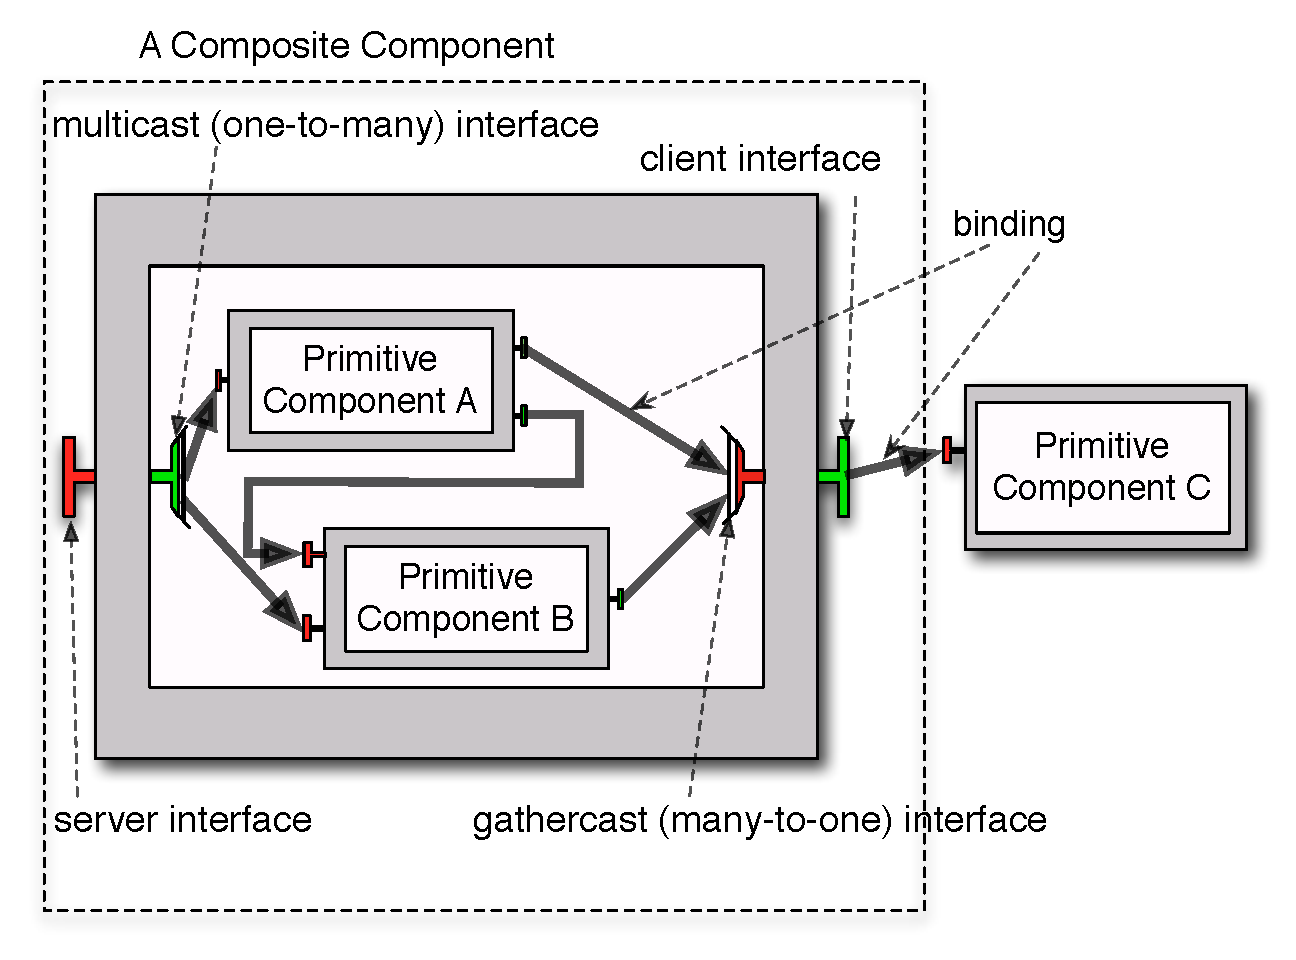
\includegraphics[scale=0.5]{figures/chapter2/gcm.pdf} 	
   		\caption{A simple GCM architecture}
   		\label{fig:gcm}
		\end{figure}
	%\end{center}		
	
		
	An example of a \gcm\ architecture is depicted by Figure \ref{fig:gcm}. Basically, the core elements
	of a \gcm\ application are (1) \textit{components}, which can be \textit{composite} or \textit{primitive} 
	---	depending on whether they have inner components or not ---, (2) \textit{interfaces}, and (3) \textit{bindings}.
	As expected, interfaces act as	access points, and bindings establish communications
	between components.
	
	Both synchronous and asynchronous communications are supported. These, can be \textit{one-to-one},
	but also of collective nature: \textit{one-to-many} (\textit{multicast}), 
	\textit{many-to-one} (\textit{gathercast}), and even \textit{many-to-many}. Moreover, support for 
	autonomic aspects are provided by means of non-functional interfaces.
	
	In the remainder of this section we delve into the \gcm\ intricacies and	
	further discuss its characteristics that are relevant for the understanding of this thesis.
	For more details the interested reader 
	is pointed to the \gcm's technical specification \cite{ETSI2010:GCM}.
	
		
	
\subsection{Overview of the GCM specification}
\label{sub:gcmspec}	
	
			
	%gcm component introspection
	%gcm component configuration --> membrane
	%gcm component instantiation
	%gcm typing			
			
			
	\paragraph{Component introspection}
	
	In the \gcm, components are endowed with introspection capabilities of its external features.	
	One of the advantages of being a hierarchical component model is the 
	possibility to  adjust the granularity of abstraction, i.e. components can be seen as white 
	or black boxes. As a black box, one cannot see its internal structure, solely its
	external interfaces. 
	
		Each interface has a name. All external interfaces of one component must have distinct names,
	but no such restriction is imposed on interfaces belonging to different components. Moreover,
	an interface is also characterized by its \textit{role}: it can be a \textit{client} or \textit{server}
	interface. The former emits operation invocations, while the latter receives them. Intuitively, 
	one should see the client interfaces as the means for service methods to interact with other
	service methods.
			
				%introspected is a correct word..
				Component's interfaces can be introspected through two different \ac{API}s: the 
			\textsf{Component} interface, and the \textsf{Interface} interface. The former
			specifies the methods \textsf{getFcInterfaces()} and \textsf{getFcInterface(string iftName)},
			that return an array of references to the component's interfaces, and a reference
			to the interface whose name matches the value \textsf{itfName} passed as argument, respectively.
			The latter, focuses on the introspection from an interface perspective. In particular, it
			specifies a \textsf{getFcItfName()} method, that returns a string with the name of the interface,
			and \textsf{getFcItfOwner()}, that returns the \textsf{Component} reference of the component
			to which it belongs.
			
			
	%membrane stuff / reconfig ...
	\paragraph{Component configuration}
		
			A \ac{GCM} component, primitive or composite, is arranged by two parts: a 
	\textit{membrane} and a \textit{content}. The former --- see the grey parts of each
	component of Figure \ref{fig:gcm} --- contains a set of controllers	that expose 
	non-functional interfaces. These allow to dynamically reconfigure the structure
	of a \ac{GCM} application. The latter, is either an object --- for primitive components ---
	or a finite set of subcomponents --- for composite components ---, 
	which are under control of the enclosing component's controllers.
	
		A membrane can have interfaces of \textit{external} and \textit{internal} \textit{visibility}. 
	External interfaces are available from outside the component, while internal interfaces
	are accessible to the component's direct subcomponents. A component's interfaces
	can share the same name provided they have a different visibility.	 Moreover,
	interfaces are also classified regarding their \textit{functionality}: they can be
	\textit{functional} or \textit{control}. The former corresponds to an interface
	providing or requiring a functionality to the component. Intuitively, it means it
	is part of the application logic. The latter provides "non-functional" aspects, 
	such as reconfiguration capabilities. This capacity to reconfigure the application's
	architecture at runtime is of paramount importance, and plays a key role in the
	realm of autonomic computing.
	
		A \textit{binding} is a communication path from a client interface to a server interface. There
	are three types of bindings. A \textit{normal} binding (1) is established between
	two external interfaces from components at the same hierarchical level, i.e.	
	possessing the same enclosing component. An \textit{import} binding	(2)	
	is made from a (sub)component to its enclosing component. Last, an \textit{export} binding (3)
	binds a component to one of its subcomponents. For the sake of clarity, these 
	are depicted by Figure \ref{fig:normal}, Figure \ref{fig:import}, and Figure \ref{fig:export}, respectively.			
			
	\begin{figure}[H]
	\begin{minipage}[b]{0.3\linewidth} 
	\centering
	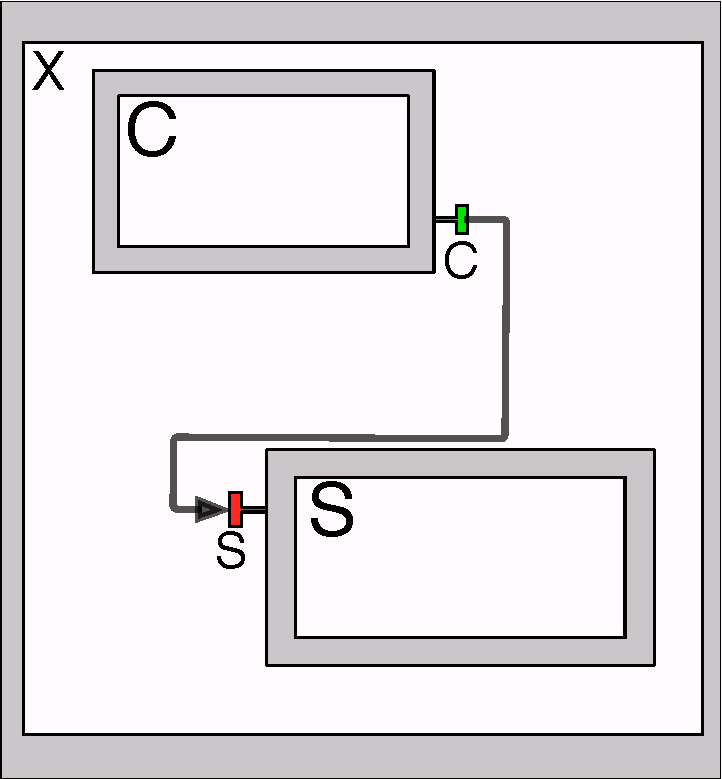
\includegraphics[width=\textwidth]{figures/chapter2/normalbinding.pdf}
	\caption{Normal Binding}
	\label{fig:normal}
	\end{minipage}
	\hspace{0.25cm}
	\begin{minipage}[b]{0.3\linewidth} 
	\centering
	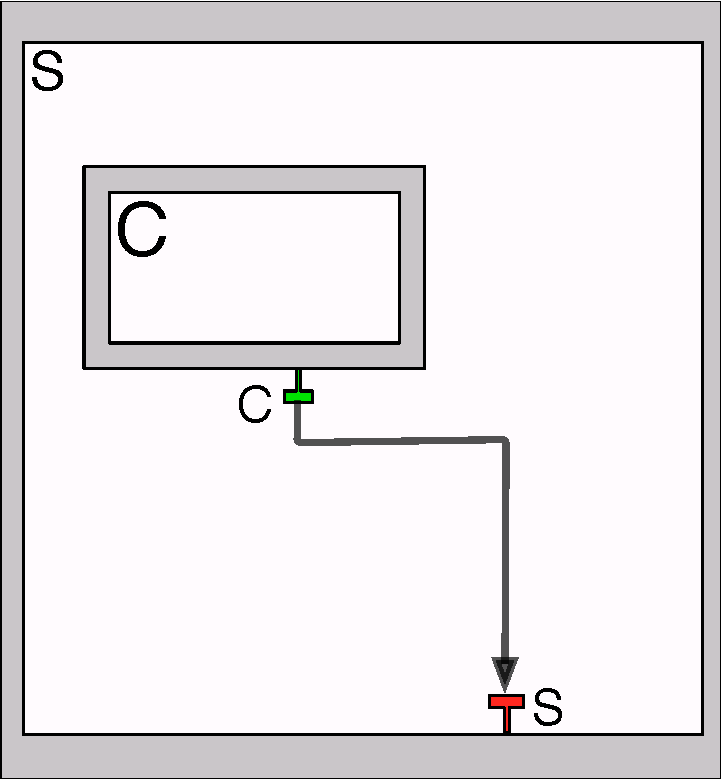
\includegraphics[width=\textwidth]{figures/chapter2/importbinding.pdf}
	\caption{Import Binding}
	\label{fig:import}
	\end{minipage}
	\hspace{0.25cm}
	\begin{minipage}[b]{0.3\linewidth}
	\centering
	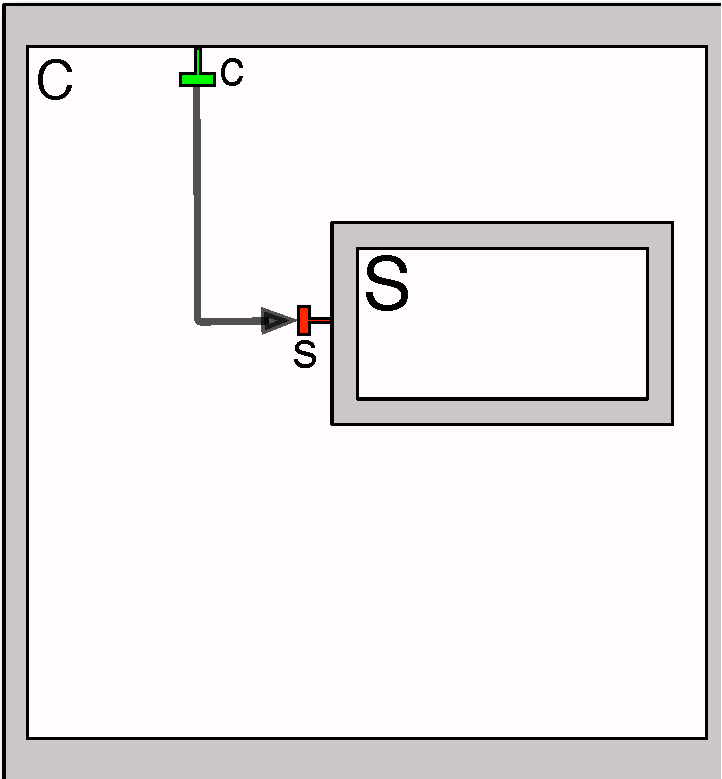
\includegraphics[width=\textwidth]{figures/chapter2/exportbinding.pdf}
	\caption{Export Binding}
	\label{fig:export}
	\end{minipage}
	\end{figure}	  		
	
	
	\noindent This can be seen as a structural constraint ensuring that no binding can "cross" a
	component boundary except through its interfaces. Further, a client interface
	can be bound to at most one server interface, while several client interfaces can be bound to the
	same server interface. This constraint is relaxed if the client interface is of \textit{multicast} 
	\textit{cardinality}. Other cardinality values include \textit{singleton}, for simple one-to-one
	communications, and \textit{gathercast} that act as a \textit{rendez-vous} for gathering data.
		
	
	\paragraph{Component runtime instantiation}
		
		In the \ac{GCM}, component creation is achieved through \textit{factories}. Basically,	
	components are created by other special type of components called 
	component factories. 

		The \ac{GCM} offers a generic component factory and a standard component factory. 
	The former allows the creation of several kinds of components, while the latter is more
	specific, it can only create components of the same type.  %Both provide
	%a \textsf{newFcInstance(...)} method, allowing the creation of new components.
	For both factories, one can wonder: \textit{if components are created from component factories,
	how are component factories created? From other component factories?} Indeed, this would lead
	to an infinite recursion. This is solved by the inclusion of a \textit{bootstrap} component factory 
	that needs not to be created explicitly. Naturally, it is able to create several kinds of components,
	namely component factories. 				
		
		
	\paragraph{Component typing}
	
			A simple type system is defined for composing components. It mainly reflects the characteristics
		of the component's interfaces. In particular it focuses on the \textit{cardinality} and \textit{contingency}
		attributes of an interface.	
					
			There are four possible values for an interface cardinality. Considering an interface of type \textbf{T}, 	
		it can be \textit{singleton} (1), entailing that the component owning it must have exactly one interface of
		type \textbf{T}. \textit{Collection} (2), indicating that an arbitrary number of interfaces of type \textbf{T}
		can coexist on a given component. However, their name must begin with the same name specified in \textbf{T}.
		Since there is an infinite number of such interfaces, they cannot be created at the same time, they must
		be created lazily, i.e., at invocation time. An interface may also be \textit{multicast} (3): it is like a singleton,
		but transforms each invocation into a set of invocations. At last, an interface of \textit{gathercast} (4) cardinality
		also behaves as a singleton, but transforms a list of invocations into a single invocation.
	    		
					
			Regarding the interface's contingency attribute, an interface can be \textit{optional} or \textit{mandatory}.
		The operations of an optional interface are not guarantee to be available at runtime, while a mandatory interface
		provides such guarantee. Basically, mandatory interfaces are made for components absolutely requiring other components
		to work, whereas optional interfaces are useful for components that may use others, if present. For instance,
		a parser component absolutely needs a lexer component, but can work with or without a logger component.
			
	
\subsection{The GCM ADL}
\label{sub:gcmadl}

		
		One may need to define arbitrarily complex architectures. With the 
	increase of complexity in the system to be described, it is important to have a precise way
	to describe such architectures. In the realm of component-based engineering, this is usually achieved 
	by means of an \adl. The \gcm\ follows this approach by supporting
	its own \gcm\ \adl\ \cite{ETSI2009:GCMADL}. 
	
		The \gcm\ \adl\ is a XML-based language. As a root element it 
		contains the \textit{definition} element. Basically, it describes the structure of the application
		via \textit{component}, \textit{interface} and 
		\textit{binding} elements. The component element possesses a \textit{name} and 
		\textit{definition} attribute. These identify the component, and its owner, respectively.
	   Moreover, it may contain the following child elements:
	   
	   \begin{itemize}
	   		\item \textit{comment}: a free form of text documenting the component. (0-unlimited);
	   		
	   		\item \textit{interface}: description of the interface provided by the component. (0-unlimited);
	   		
	   		\item \textit{component}: reference to a subcomponent. (0-unlimited);
	   		
	   		\item \textit{binding}: description of the binding hold by the component. (0-unlimited);
	   		
	   		\item \textit{content}: class which represents the components. (0-1);
	   		
	   		\item \textit{attributes}: list of attributes of the component. (0-1);
	   		
			\item \textit{controller}: controller of the component. (0-1);
			
			\item \textit{virtualNodes}: 	list of virtual nodes the component should be deployed on. (0-1);
			
			\item \textit{exportVirtualNodes}:  list of export virtual nodes. (0-1)	.
	   		
		\end{itemize}	   	

	\noindent A \textit{comment} element is a simple text element, adding some contextual
	information.	 An \textit{interface} element possesses the following attributes:
	
	
		\begin{itemize}
			\item \textit{name}: identifier of the interface. (required);
			
			\item \textit{role}: 'client' or 'server'. (required);
			
			\item \textit{signature}: signature of the interface. (required);
			
			\item \textit{contingency}: 'mandatory' or 'optional'. (optional);
			
			\item \textit{cardinality}: 'singleton', 'collection', 'gathercast' or 'multicast'. (optional);
						
			\item \textit{comment}: a free form of text documenting the interface. (0-unlimited).
		\end{itemize}	
	
		\noindent Its constituting attributes should pose no doubt. However, the 
		careful reader may notice that there is no attribute specifying whether an interface is
		of internal or external visibility. This must be handled in an automated manner. For instance,
		a multicast server interface of a composite component is in fact the composition
		between a server interface and a multicast internal client interface.	
	
		Next, the component child element of the component element portrays 		
	   \ac{GCM}'s hierarchical nature.	 The binding element is solely composed by two attributes,
	   \textit{client} and \textit{server}, which hold the name of the client and server interfaces involved
	   in the binding, respectively. The content element features solely the \textit{class} attribute that specifies
	   the class implementing the component. 
	   
	   	The \textit{attributes} element  are key/value pairs that can be used to parametrize the component.
		The \textit{controller} element indicates the component controller that manages the component
		w.r.t. non-functional aspects. 	Finally, the remaining elements \textit{virtualNodes} and \textit{exportVirtualNodes}
		serve the purpose of facilitating the deployment task, i.e., one may want to distribute its application
		to a set of predefined nodes.   


		%non-functional interfaces
		%autonomic computing, Component membrane
		%ruz, oleksandra


		
			This Subsection discussed the main ingredients of the \ac{GCM} \ac{ADL}. For a more detailed
		description of its intricacies, namely its XML schema, 
		the interested reader is pointed to its technical specification \cite{ETSI2009:GCMADL}.	
				
	

\section{ProActive --- A middleware for distributed programming}
\label{sec:proactive}

		ProActive\footnote{Available online: \url{http://proactive.activeeon.com/index.php}} is an open 
	source Java middleware for the programming of multi-threaded, parallel, and distributed 
	applications. An application adopting ProActive is composed by entities denominated \textit{active objects} \cite{AO2007}. Each active object
	contains a distinguished element, the \textit{root}, that is its only entry point. Moreover, it possesses
	its own thread of control, every incoming method call is automatically placed in a queue of pending requests,
	and is able to decide by which order it serves them. 
			
			%placeholder is correct word
		Further, incoming method calls are asynchronous with transparent \textit{future} objects. 
	Basically, a short \textit{rendezvous} occurs at the beginning of each	asynchronous remote call, which blocks
	the caller until the call has reached the callee. Then,	if the invoked method returns a result, a future object is
    created on the callee side and returned back as a result to the caller. Thus, a future
	can be seen as a placeholder for the return value of an active object method invocation. 
	The object that issued the invocation can therefore proceed its execution. At a later stage,
	if it needs to read the actual returned value, it blocks until the value is available --- i.e. until
	the request is processed and returned back from the callee --- or continues transparently
	if meanwhile the value has already been obtained. This mechanism is called 
	\textit{wait-by-necessity}.

		Another common nomenclature found in the literature for the future concept 
	is \textit{promise} \cite{AO2007}. Both terms are often used interchangeably.
	

\subsection{GCM/ProActive --- a reference implementation for GCM}
\label{sub:gcmpro}


		As mentioned earlier, ProActive is the \textit{de facto} reference implementation for \ac{GCM}.
	For this reason, whenever focusing on its component model part, it is often referred 
	to by GCM/ProActive.

		In GCM/ProActive a primitive component is implemented through an active object, and 
	thus includes its standard features. Components communicate asynchronously 
	through the established bindings between their interfaces. 
	
	
		For instance, let us consider two components of some architecture as depicted by Figure 
	\ref{fig:asynch1}. Components \textbf{A} and \textbf{B} both possess a server interface (in red),
	and the former is also equipped with a client interface (in green). A binding between
	\textbf{A}'s client interface and \textbf{B}'s server interface connects them together.
	Moreover, they both include a request queue.	
	
	\begin{figure}[H]
	\begin{minipage}[b]{0.5\linewidth} 
	%\centering
	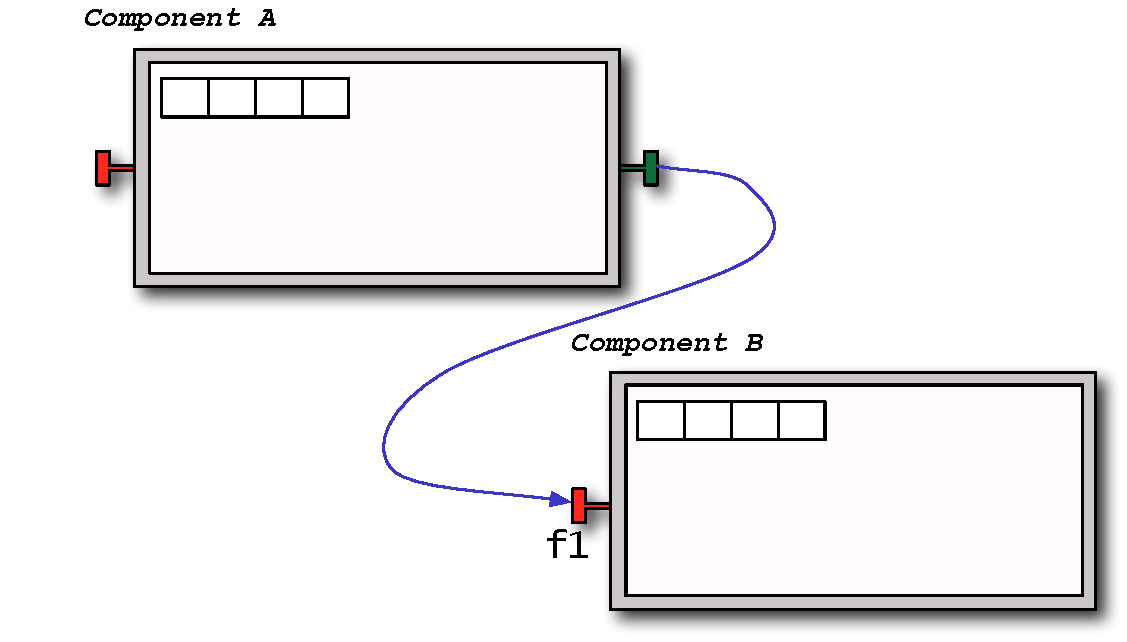
\includegraphics[width=\textwidth]{figures/chapter2/asynch1.pdf}
	\caption{Components \textbf{A} and \textbf{B}}
	\label{fig:asynch1}
	\end{minipage}
	%\hspace{0.25cm}
	\begin{minipage}[b]{0.5\linewidth} 
	%\centering
	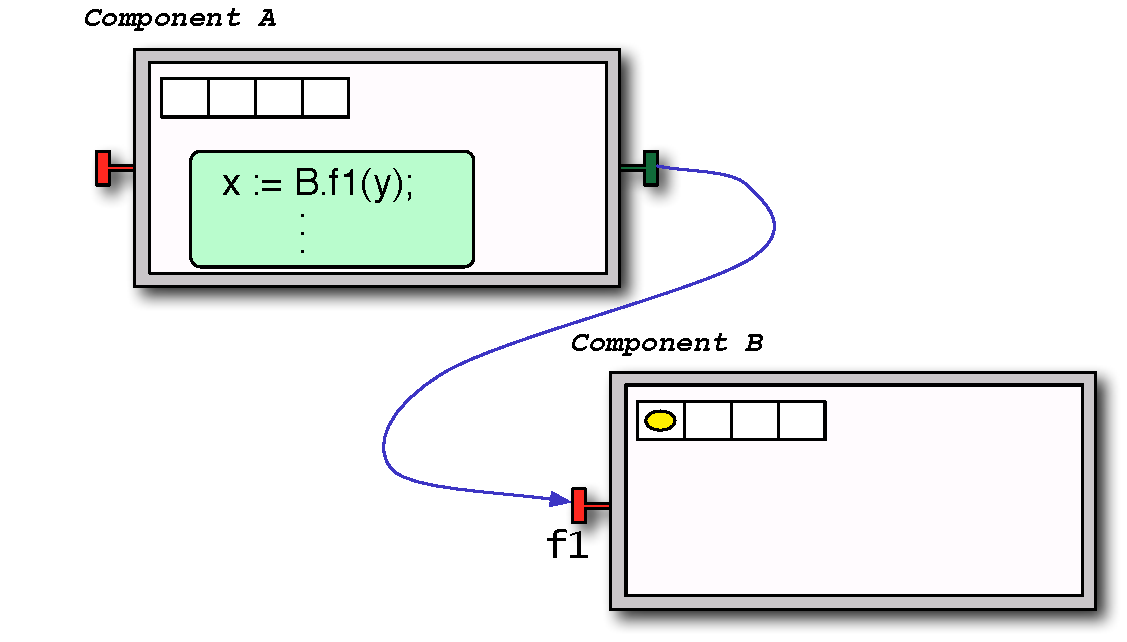
\includegraphics[width=\textwidth]{figures/chapter2/asynch2.pdf}
	\caption{\textbf{A} invokes \textbf{f$_1$} from \textbf{B}}
	\label{fig:asynch2}
	\end{minipage}
	\end{figure}	 
		
	\noindent Whenever \textbf{A} invokes the method \textbf{f$_1$} from \textbf{B}'s
	server interface, a request is inserted into \textbf{B}'s queue.
	At this point, the variable \textbf{x} holds a future for the reply of \textbf{f$_1$},
	and \textbf{A} proceeds its execution (Figure \ref{fig:asynch2}). 
		
	
	
	\begin{figure}[H]
	\begin{minipage}[b]{0.5\linewidth} 
	%\centering
	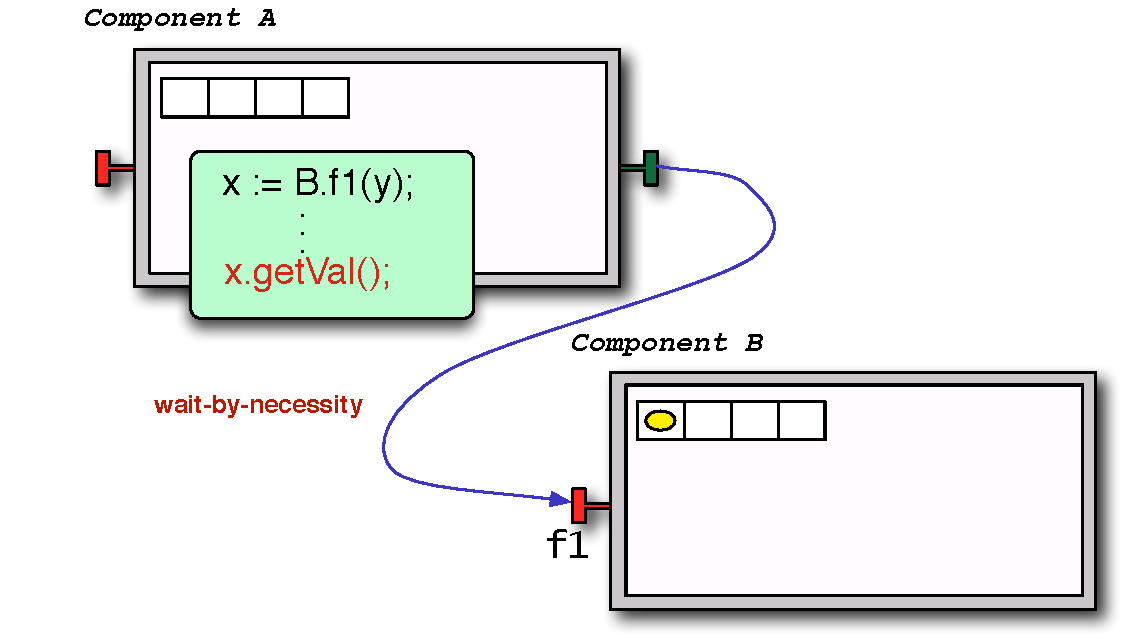
\includegraphics[width=\textwidth]{figures/chapter2/asynch3.pdf}
	\caption{\textbf{A} blocks! \textit{wait-by-necessity}}
	\label{fig:asynch3}
	\end{minipage}
	%\hspace{0.25cm}
	\begin{minipage}[b]{0.5\linewidth} 
	%\centering
	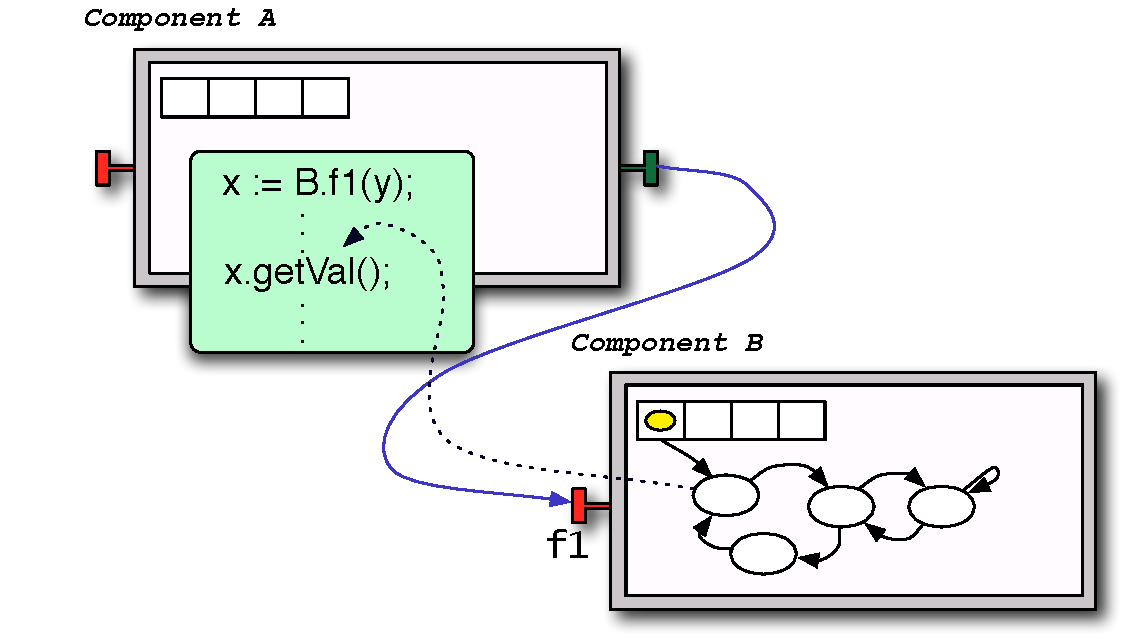
\includegraphics[width=\textwidth]{figures/chapter2/asynch4.pdf}
	\caption{\textbf{B} replies, and \textbf{A} is happy}
	\label{fig:asynch4}
	\end{minipage}
	\end{figure}	 	
	
	
	\noindent If \textbf{A} needs to access the value of \textbf{x}, then it may be the
	case that \textbf{B} has not yet treated the request, and thus \textbf{A} blocks
	until it gets the reply from \textbf{f$_1$}'s invocation (Figure \ref{fig:asynch3}).
	Alternatively, it may be the case that \textbf{B} already replied,
	and therefore \textbf{A} can proceed its execution transparently (Figure \ref{fig:asynch4}).
	
	
		As expected, \ac{GCM} components are mono-threaded, i.e. only one request is treated at a time.
	It may seem restrictive, but it has the benefit of ensuring thread-safety. Nevertheless,
	we may refer that recent work aims at improving performance by allowing multi-threading
	for active objects \cite{henrio:hal-00818482}.
	
	
\subsection{Specifying architectures with the ADL}
\label{sub:gcmproadl}

	
		As discussed in Subsection \ref{sub:gcmadl}, the \ac{GCM} defines its \ac{ADL} as a means
	to specify component architectures. GCM/ProActive includes support for such feature. For instance,
	let us consider the simple \ac{GCM} application depicted by Figure \ref{fig:starter}.

		%\begin{center}
		\begin{figure}[H]
		\centering
	   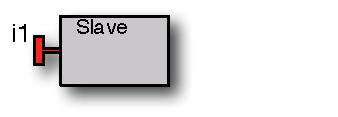
\includegraphics[scale=1]{figures/chapter2/starter.pdf} 	
   		\caption{Simple GCM application example}
   		\label{fig:starter}
		\end{figure}
	%\end{center}		


	\noindent It is composed solely by one primitive component, named \textit{Slave}, possessing one server interface
	named \textit{i$_1$}. Listing \ref{lst:starteradl} illustrates the specification of this architecture. 

\lstinputlisting[language=MyXML,
	                        stepnumber=1, caption=GCM/ProActive \textit{slave} component ADL, label=lst:starteradl]{listings/chapter2/starteradl.tex}		

		
	\noindent The contents of the \ac{ADL} should pose no doubt. Line 1 concerns \textit{XML} validation
	aspects, basically it allows standard validators to check if the \textit{XML} file is well formed.
	The component architecture aspects \textit{per se} begin at line 2. Its \textit{definition} possesses the \textit{name}
	attribute indicating its classpath, and contains three child elements: \textit{interface}, \textit{content} and \textit{controller}. 
	The interface's
	signature points to the \textit{java} interface file holding signature for the supported service methods. Next,
	it is specified as having a server \textit{role} and with name \textit{i$_1$} (line 3). The \textit{content} holds the
	\textit{class} attribute that indicates the actual \textit{java} implementation for this component. i.e. it implements
	the service methods specified in the interface's \textit{signature} (line 4). At last, the \textit{controller} specifies
	the default primitive component controller (line 5).		
		Moreover, no information is provided regarding \textit{virtual nodes}. This is usually the case when deploying
	the application locally.	


	\noindent Let us now look at a more elaborated example. Figure \ref{fig:composite} depicts a slightly more
	complex architecture featuring three components: \textit{Composite}, \textit{Master} and the previously
	discussed \textit{Slave}.

	
		%\begin{center}
		\begin{figure}[H]
		\centering
	   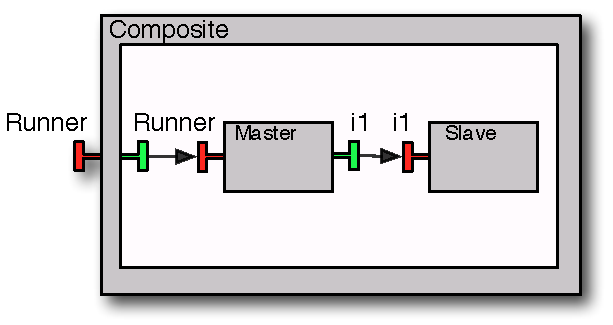
\includegraphics[scale=1]{figures/chapter2/composite.pdf} 	
   		\caption{GCM \textit{composite} application example}
   		\label{fig:composite}
		\end{figure}
	%\end{center}		
	
	
	\noindent The \textit{Composite} encapsulates the two remaining components and exposes one
	external server named \textit{Runner}. Its symmetric counterpart, i.e. internal and client, is
	bound to the server interface of the \textit{Master} component, also named \textit{Runner}. Further,
	the \textit{Master} component is also equipped with a client interface named \textit{i$_1$} that
	is bound to the \textit{Slave}'s server interface. Listing \ref{lst:cadl} shows its \ac{ADL}.
	

	
\lstinputlisting[language=MyXML,
                        stepnumber=1, caption=GCM/ProActive \textit{Composite} component ADL, label=lst:cadl]{listings/chapter2/compositeadl.tex}		

 
	\noindent Line 3 starts the \textit{definition} of this \textit{Composite} by indicating its classpath, and
	including the child elements relevant for this specification.	
	As mentioned above, the \ac{GCM} \ac{ADL} does not include an attribute for specifying whether an interface
	is of external or internal visibility. Indeed, there is only one \textit{interface} element included in the 
	\textit{composite} \ac{ADL} (line 4). Its symmetric counterpart is not specified and automatically handled by GCM/ProActive.
	Next, the \textit{component} elements at lines 6 and 7 are references to their actual \ac{ADL}s.
	Lines 9 and 10 specify the two bindings of this architecture using	the familiar \textbf{this} 
	and \textbf{.} notations. For last, line 12 specifies the \textit{controller} 
	as the default composite component controller.
	
	
	The remaining pieces for the specification of the \textit{Composite} architecture concerns
	the \ac{ADL}s of its two subcomponents: \textit{Master} and \textit{Slave}.
	The \textit{Slave} architecture has already been discussed (see Listing \ref{lst:starteradl}),
	its only modification concerns the classpath of its \textit{name} definition.
	Regarding the \textit{Master} component, its \ac{ADL} is depicted by Listing \ref{lst:madl}.
	
	
	\lstinputlisting[language=MyXML,
                        stepnumber=1, caption=GCM/ProActive \textit{Master} component ADL, label=lst:madl]{listings/chapter2/masteradl.tex}		

		
	\noindent As expected, it follows the same structure as the \textit{Slave} \ac{ADL}. Indeed,
	it mainly differs on the inclusion of a client interface (line 5).
	
	
		
	In this Section we only covered the fundamentals of the ProActive	middleware.	
	The interested reader is pointed to ProActive's programming manual for more
	discussion on its intricacies \cite{PROACTIVE2013:GCM}.		
		

%%%%%%%%%%%%%%%%%%%%%%%%%%%
\section{pNets: A formalism for defining behavioural semantics}
\label{sec:pnets}

	
		\textit{pNets} stands for \textit{parametrized Network of synchronized automata}. It provides
	an intermediate and general formalism aimed at the specification and synchronisation
	of the behaviour of a set of automata.	 Further, it is mainly aimed towards two goals:
	provide a formal foundation to the model generation principles for distributed component
	frameworks --- such as \ac{GCM} ---, and to propose an expressive, yet concise, machine-oriented 
	model that can be used as an internal format for software tools.
	
		The first definition of pNets was published in \cite{BBCHM:article2008}. Here, we restrict ourselves 
	to a more succinct discussion, focusing on the material relevant for the understanding of this thesis.	
	
		A pNet is a hierarchical structure whose leaves are \textit{pLTS}s or \textit{queues}. A pLTS is a labelled
	transition system with variables. It can possess guards and assignments on its transitions. It is formally
	defined as follows.

\begin{definition}[pLTS] 
\label{def:plts}

A pLTS is a parametrized LTS defined by a tuple $pLTS \triangleq (P, S, s_0, L, \rightarrow)$ where
\begin{itemize}
	\item P is a finite set of parameters, from which we construct the term algebra $\mathcal{T}_P$,
	         with parametrized actions $\mathcal{A}_P$, the parametrized expression $\mathcal{E}_P$,
	         and the boolean expressions $\mathcal{B}_P$.

	\item S is a set of states. For each state $s \in S$, variables of $s$ are global to the pLTS.
	
	\item $s_0 \in S$ is the initial state.
	
	\item L is the set of labels of the form $(\alpha, e_b, (x_j := e_j)^{j\in J})$, where $\alpha \in \mathcal{A}_P$
	is a parametrized action, $e_b \in \mathcal{B}_P$ is a guard, and the variables $x_j \in P$ are assigned the 
	expressions $e_j \in \mathcal{E}_P$. %Variables in $iv(\alpha)$ are assigned by the action, other variables
	%can be assigned by the additional assignments.
	%to my understanding: iv(Some_Action ? x, y) = {x, y}	
	
	\item $\rightarrow \subseteq S \times L \times S$ is the transition relation.
\end{itemize}
\end{definition}

		
	Before proceeding to the remaining 
	definition of a pNet structure, let us define the \textit{sort} of a pNet.
	Basically, it is its signature: the set of actions it can perform, 
	that is, the set of labels of its transitions. We define it by the following
	function $Sort : pNet \rightarrow \mathcal{A}_P$.

	\begin{center}
	\begin{changemargin}{0cm}{-2cm}		
		$Sort(p) = \left\{ \begin{array}{ll}
           L & \mbox{for} \ p =(P, S, s_0, L, \rightarrow)       \\ 
           \{ ?Q\_m_i \ | \ m_i \in \mathcal{M}\} \cup \{ !Serve\_m_i \ | \ m_i \in \mathcal{M}\} & \mbox{for} \ p = Queue(\mathcal{M})\\
           L                           & \mbox{for} \ p = (P, L, pNet_i^{k \in K}, SV_k^{k \in K})
        \end{array}\right.$      
	\end{changemargin}	 
	\end{center}
	
	
	\noindent  Its definition should pose no doubt. For the cases of being a leaf, 
	if it is either a pLTS or a queue. For the former it simply returns 
	its set of labels $L$. For the latter it returns a set of actions 
	depending on $\mathcal{M} \subseteq \mathcal{T}_P$. Basically, a $Queue(\mathcal{M})$ 
	can be seen as an infinite pLTS modelling the behaviour of a \ac{FIFO} queue. 
	Its semantics is simply the en-queueing and de-queueing of
	$m_i \in \mathcal{M}$. The last case concerns the recursive constructor of
	the pNet structure, where we also simply return its set of labels $L$.
	
			Let us now see a formal definition for pNet.	

	\begin{definition}[pNet]
	\label{def:pnet}	
	A pNet is a hierarchical structure defined by 
	$pNet \triangleq pLTS \ | \ Queue(\mathcal{M}) \ | \ (P, L, pNet_i^{i \in \mathcal{I}}, SV_k^{k \in K})$ where
	
	\begin{itemize}
		\item P is a finite set of parameters, from which we construct the term algebra $\mathcal{T}_P$, with
		parametrized actions $\mathcal{A}_P$.
		
		\item $L \subseteq \mathcal{A}_P$ is the set of labels actions of the pNet.
		
		\item $\mathcal{I} \in \mathcal{I}_P$ is the set of over which sub-pNets are indexed, $\mathcal{I} \neq \emptyset$.
		
		\item pNet$_i^{i \in \mathcal{I}}$ is the family of sub-pNets.
		
		\item SV$_k^{k \in K}$ is a set of synchronization vectors $(K \in \mathcal{I}_P)$. 
		$\forall k \in K, SV_k = \alpha_j^{j \in J_k} \rightarrow \alpha'_k$. Each synchronization
		vector verifies: $\alpha'_k \in L, J_k \in \mathcal{I}_P, \emptyset \subset J_k \subseteq I$, and
		$\forall j \in J_k. \alpha_j \in Sort(pNet_j)$.
		
	\end{itemize}
	\end{definition}

	\noindent Being a hierarchical structure, a pNet composes sub-pNets and expresses by its
	synchronization vectors how the sub-entities are synchronized. For instance, 
	$SV_k = \alpha_j^{j \in J} \rightarrow \alpha'_k$
	means that each sub-pNet can perform the action $\alpha_j$, resulting in a global
	action labelled $\alpha'_k$.
	

	%%assumptions pp 14
	
%%\label{TODO:ludovic}
%add details on the semantics;
%what is synchronous?
%what about parametrized families?
\subsection{Behavioural semantics for GCM/ProActive applications}
\label{sub:pnetsgcm}


		Section \ref{sec:gcm} presented the \ac{GCM}, and its reference implementation
	was discussed in Section \ref{sec:proactive}. Here, we show how to use pNets to
	give a formal semantics to GCM/ProActive applications.
	
		%First, let us define some ...
	
		As an illustrative example, the internals of a GCM primitive component featuring three service methods 
		--- \textsf{m$_1$}, \textsf{m$_2$} and \textsf{m$_3$} --- 
	and two client methods --- \textsf{m$_4$} and \textsf{m$_5$} --- are depicted by Figure \ref{fig:pnetp}. 
	
	\begin{figure}%[H]
		\centering
	   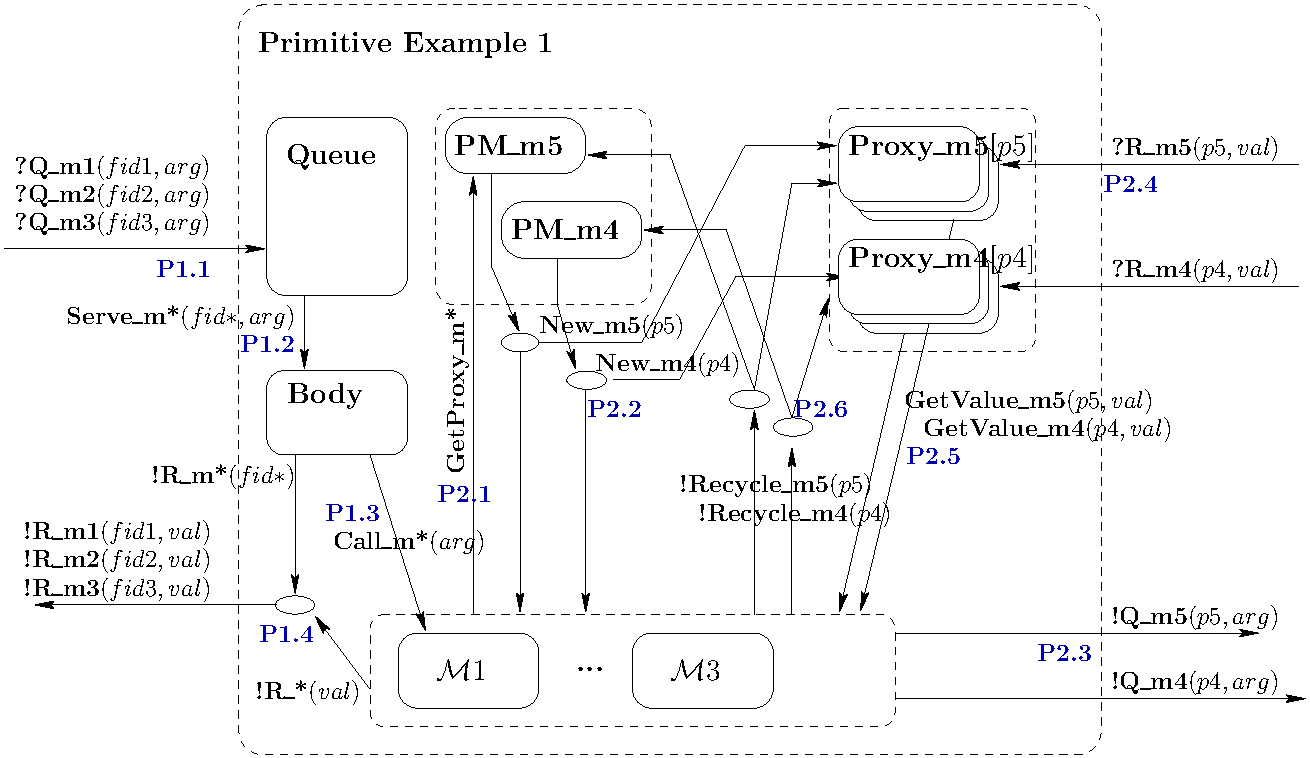
\includegraphics[scale=0.6]{figures/chapter2/pNets-primitiveComponent.eps} %0.35   		
   		\caption{pNet representing a primitive component}
   		\label{fig:pnetp}
		\end{figure}		
	
	
		\noindent Invocation on service methods --- \textsf{Q\_m$_{i, \ i \in \{1, 2, 3\}}$} --- go through 
		a \textsf{Queue}, that dispatches the request ---
	\textsf{Serve\_m*} --- to the \textsf{Body}. Serving the request consists in performing a \textsf{Call\_m*} to the
	adequate service method, represented by the $\mathcal{M}_i$ boxes in the figure. Once a result is computed, a 
	synchronized \textsf{R\_m*} action is emitted. This synchronization occurring between the service method and the
	\textsf{Body} stems from the fact that GCM primitive components are mono-threaded. Moreover, the careful reader will
	notice the $fid_{i, \ i \in \{1, 2, 3\}}$ in the figure. These are the previously discussed \textit{futures} (see Section \ref{sec:proactive}), 
	and act as promises for replies, leveraging
	asynchrony between components.
	
		Service methods interact with external components by means of client interfaces. This requires obtaining a proxy
		--- \textsf{GetProxy\_m*}, \textsf{New\_m$_{i, \ i \in \{4, 5\}}$} --- in order to be able to invoke client methods ---
		\textsf{Q\_m$_{i, \ i \in \{4, 5\}}$}. The reply --- \textsf{R\_m$_{i, \ i \in \{4, 5\}}$} --- goes to the proxy used to 
		call the external component. Then, a \textsf{GetValue\_m$_{i, \ i \in \{4, 5\}}$} is performed in order to access
		the result in the method being served. Finally, \textsf{Recycle\_m$_{i, \ i \in \{4, 5\}}$} actions can be performed
		in order to release the proxies.
	
		The behaviour of the \textsf{Queue} and the \textsf{Body} elements should pose no doubt. The former acts as
		a queue with a \ac{FIFO} policy, raising an exception if its capacity is exceeded. 
		The latter dispatches the requests to the appropriate
		method and awaits its \textit{return}, thus preventing the service of other requests in parallel.
	
		
	
	\begin{figure}%[H]
	\begin{minipage}[b]{0.4\linewidth} 
	\centering
	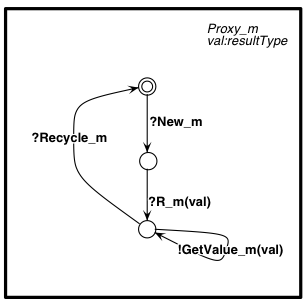
\includegraphics[width=\textwidth]{figures/chapter2/proxy.png}
	\caption{Behaviour of proxy}
	\label{fig:proxy}
	\end{minipage}
	\hspace{0.25cm}
	\begin{minipage}[b]{0.4\linewidth} 
	\centering
	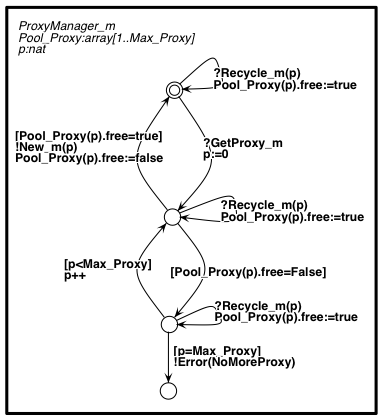
\includegraphics[width=\textwidth]{figures/chapter2/pm.png}
	\caption{Behaviour of the proxy manager}
	\label{fig:pm}
	\end{minipage}
	\end{figure}	  		
	
	
	The handling of proxies however, is not as straightforward and deserves a closer look.
	Figures \ref{fig:proxy} and \ref{fig:pm} illustrate the behaviour of the \textsf{Proxies} and \textsf{Proxy Managers}, respectively. 
	Upon reception of a \textsf{New\_m$_i$} action, a \textsf{Proxy} waits for the reply of the method invoked with it --- \textsf{R\_m} ---,
	making thereafter its result available --- \textsf{GetValue\_m}.  As soon as the reply is
	received, the \textsf{Proxy} can potentially be recycled through a \textsf{Recycle\_m}
	action.
				
		The behaviour of the \textsf{Proxy Manager} is slightly more elaborated. It maintains a \textit{pool} of proxies, keeping track of 
  those available and those already allocated. On the reception of a \textsf{GetProxy\_m} action, it activates a new proxy 
  --- \textsf{New\_m} --- if there is one available. Should that not be the case, an \textsf{Error(NoMoreProxy)} action is emitted.  
	As expected, a \textsf{Recycle\_m} action frees a previously allocated proxy. 	
	
	
\subsection{Coping with structural reconfigurations}
\label{sub:reconfig}	


		As mentioned in Section \ref{sec:gcm}, the \ac{GCM} also contemplates non-functional
	aspects such as structural reconfigurations. This means that the architecture
	of the application can evolve at runtime (e.g. by establishing new bindings, 
	removing existing ones, ...).
		
	For \ac{GCM} applications \textit{bind} and \textit{unbind} operations are handled by the component
	owning the \textit{client} interface that is supposed to be reconfigurable. This should come
	as no surprise, indeed, it follows the same spirit as in object-oriented languages: an object
	holds the reference to a target object; it is this object that must change the reference it holds.
	Moreover, we recall that client interfaces can be of singleton or multicast cardinality.
	The former is bound to at most one server interface, while the latter needs to potentially 
	handle several recipients. Therefore, their reconfiguration is dealt in different manners. 
	
	Let us first illustrate how a reconfigurable client singleton interface is modelled in \textit{pNets}. 
	A component is equipped with a \textit{binding controller} interface to bind and unbind	its
	client singleton interfaces. As depicted by Figure \ref{fig:bc}, the binding controller pLTS attached
	to each of them controls their bindings.
	
	
\begin{figure}%[H]
		\centering
		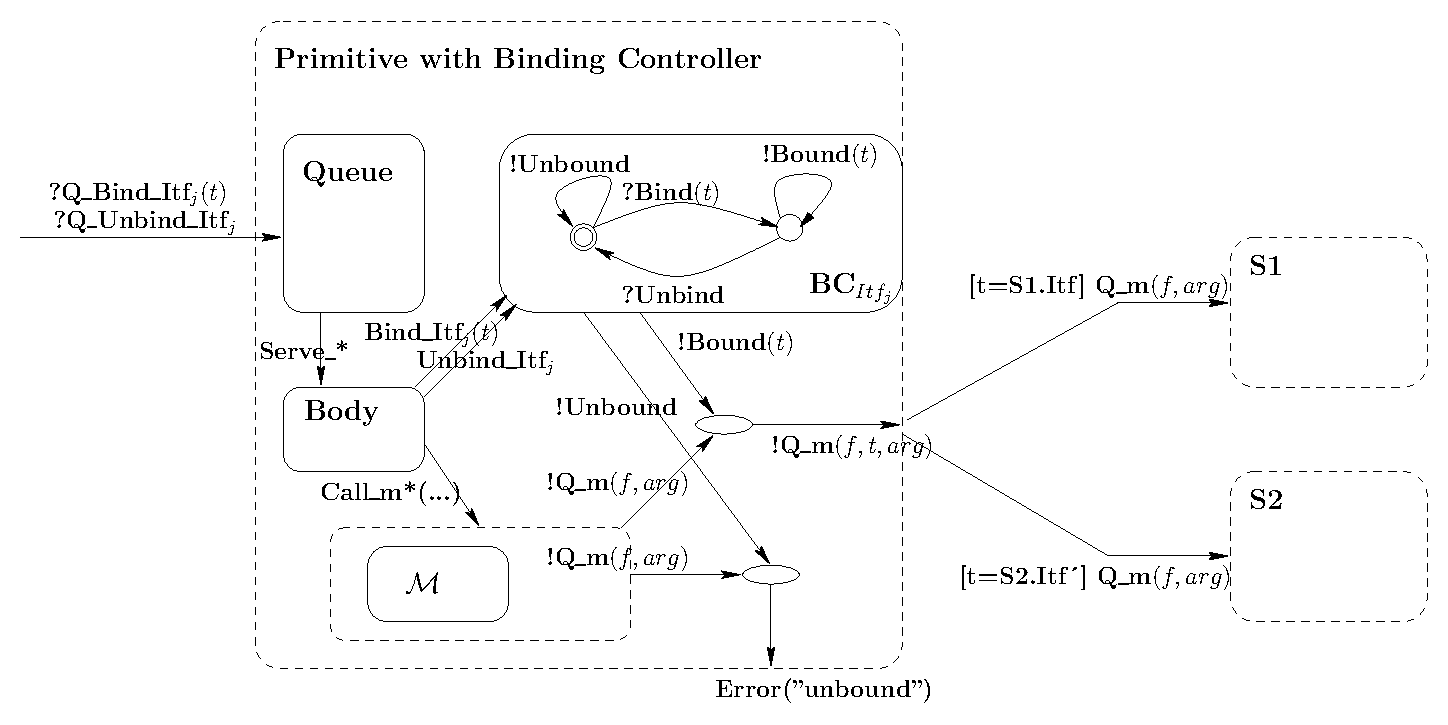
\includegraphics[scale=0.5]{figures/chapter2/pNets-primitiveBC.eps}
		\caption{Binding controller}
		\label{fig:bc}		
\end{figure}	

	Indeed, we allow for reconfigurations by defining two new request messages for the \textit{binding} and \textit{unbinding}
		of interfaces. These are delegated to a binding controller that upon method invocation over these
		reconfigurable interfaces will check if they are indeed bound, emitting an error if it is not the case. Moreover, the 
		target of the invocation is decided by checking its passed reference. For this reason one must know statically what are the 
		possible target interfaces that a reconfigurable interface can be bound too.
	

%%$ multicast

	  Reconfigurations involving multicast interfaces require keeping track of a set of recipients.	  
	  Figure \ref{fig:mc} depicts the pNet specificities concerning the handling of such interfaces.


\begin{figure}[H]
		\centering
		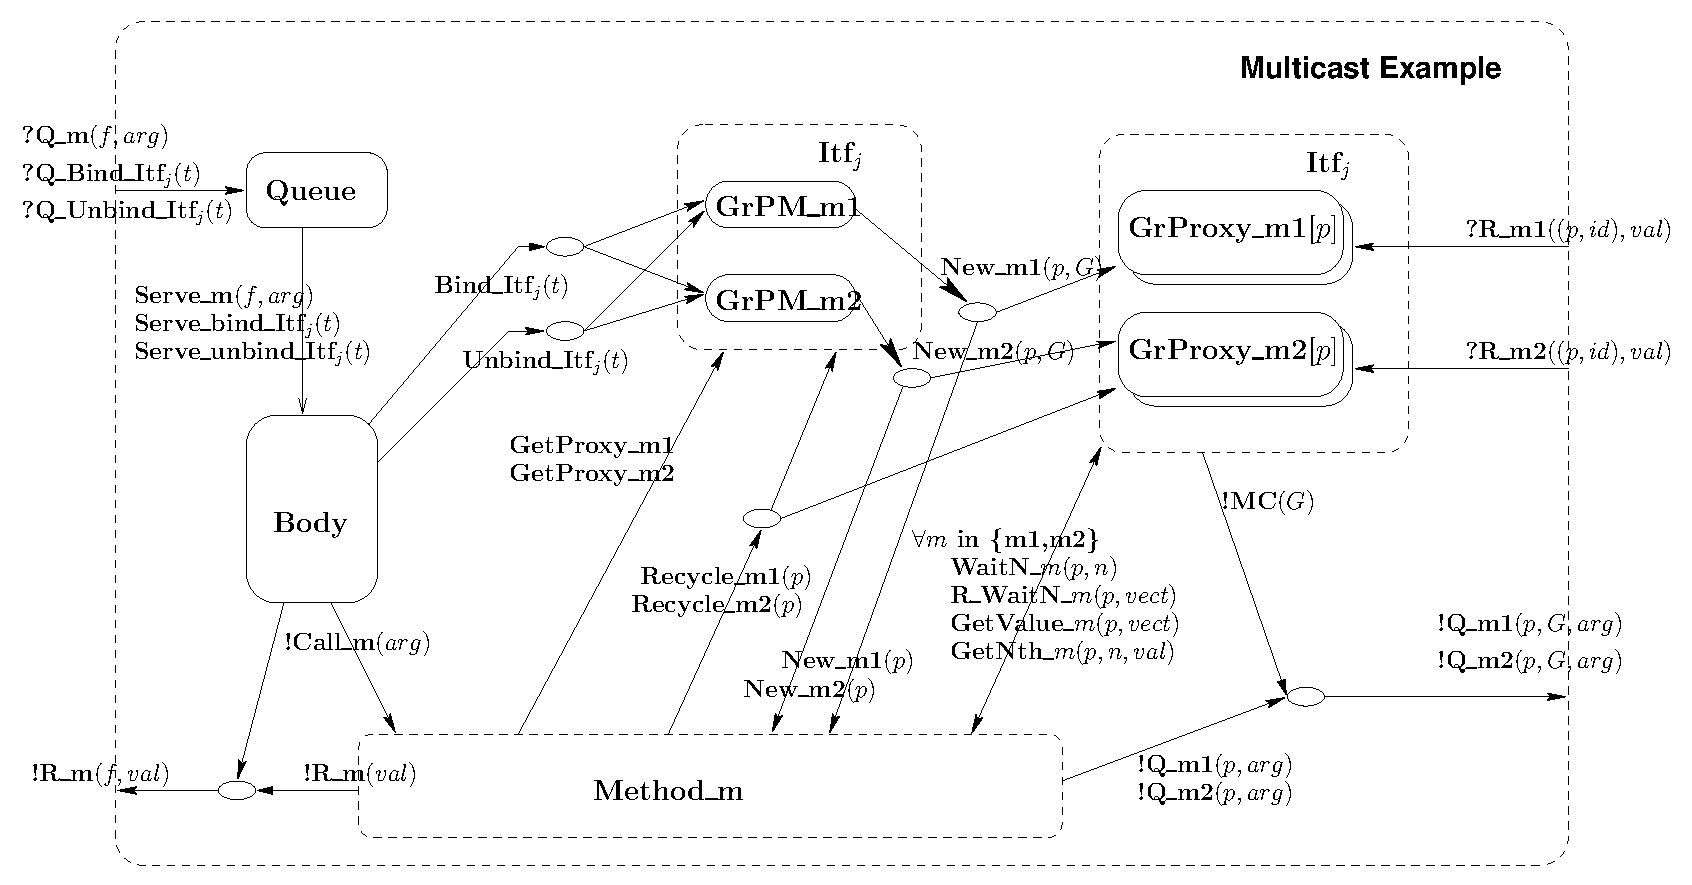
\includegraphics[scale=0.45]{figures/chapter2/pNets-MulticastExample.eps}
		\caption{pNet example for reconfigurable multicast interface}
		\label{fig:mc}		
\end{figure}	


			\noindent In short, the machinery involved for dealing with this kind of interfaces mainly differs from
		reconfigurable singleton interfaces in that we must keep track of the target's connectedness status. 
		Indeed, the emission of a new proxy --- \textsf{New\_m$_{i, i \in \{1, 2\}}$} --- is synchronized in a similar manner, however
		we also transmit the current status of the multicast interface (i.e. the \textsf{G} variable in the figure).
		This status will be taken into account when invoking one of the client methods --- \textsf{Q\_m$_{i, i \in \{1, 2\}}$}.
		In practice, \textsf{G} is a boolean vector whose element's valuation determine the interface's connectedness. 


		In this section we succinctly presented pNets mainly focusing on its application to the 
		formal specification of \ac{GCM} applications. It should be noted however, that 
		pNets is also suited for the specification of other types of systems.
		For a more detailed account on its intricacies the interested reader is
		pointed to its authoritative reference \cite{BHMS:RRBeh-2012}.
	



%%%%%%%%%%%%
\section{The Fiacre specification language}
\label{sec:fiacre}

	\textit{Fiacre} \cite{fiacre2009} stands for 
	\textit{Format Interm\'ediaire pour les Architectures de Composants R\'epartis Embarqu\'es}. 
	It is a formal language that allows to model systems,
	in particular, embedded and distributed systems, for formal verification and 
	simulation purposes.
	
	It is built around two notions: \textit{processes} and \textit{components}. The former
	describes the behaviour of sequential components. It is defined by a set of states,
	each associated with a program made of standard programming language constructs 
	(loops, if-then-else, ...), non-deterministic constructs, communication events, and
	jumps to subsequent states. The latter describes the composition of processes. It is defined
	as a parallel composition of components and/or processes communicating through ports
	and shared variables.

	For the sake of clarity, let us see a simple example\footnote{The described example
	is a slight adaptation from the online Fiacre tutorial: 
	\url{http://projects.laas.fr/fiacre/doc/fiacre-tutorial.html}}. First, we define
	an \textit{union} type as depicted by Listing \ref{lst:ordertype}.
	
	\lstinputlisting[language=Fiacre,
	                        stepnumber=1, caption=The \textsf{Order} type, 
	                        label=lst:ordertype]{listings/chapter2/type.fiacre}		
			

	\noindent Basically, the above \textsf{Order} type encodes two types of orders:
	make a sandwich (line 2), that takes no parameter as we assume there is only one kind
	of sandwich, and to make coffee (line 3), that takes a value ranging over [0..2]
	symbolizing that there are three kinds of coffee. 
	
	Let us now see a first Fiacre process. Listing \ref{lst:process1} encodes
	the beginning of the \textsf{Slave} process.
	
	\lstinputlisting[language=Fiacre, firstnumber=5,
	                        stepnumber=1, caption=The Slave process (part 1/2), 
	                        label=lst:process1]{listings/chapter2/process1.fiacre}	

	\noindent The \textsf{Slave} process takes two parameters, often called \textit{labels}.
	As we shall see later, these are used to make processes communicate together,
	or more precisely, \textit{synchronize}.
	
	At line 5, we can see that the first parameter, \textsf{ready}, is declared with type \textsf{none}. 
	It is a predefined
	type meaning that no value can be attached to it. The second parameter, \textsf{order},
	is  of \textsf{Order} type.	 Moreover, the \textsf{in} keyword stands for the fact that it can
	only receive orders, and not emit them.

	From line 6 to line 8 we define all the states of the \textsf{Slave} process. Further, a local variable,
	\textsf{tmp}, of type \textsf{Order}, is defined at line 9. We can now proceed to the
	 the process behaviour. Listing \ref{lst:process2} depicts its definition.

	\lstinputlisting[language=Fiacre, firstnumber=10,
	                        stepnumber=1, caption=The Slave process (part 2/2), 
	                        label=lst:process2]{listings/chapter2/process2.fiacre}	

	\noindent Its understanding should pose no doubt, as the Fiacre specification language
	is rather intuitive and concise. 
	
	From its initial state, \textsf{startSlavery}, upon reception of a
	\textsf{ready} message (lines 10-11), the process proceeds
    to the \textsf{waitOrder} state (line 12). From there, it awaits
    for an \textsf{order} message, and stores its value on the \textsf{tmp}
    variable (lines 14-15). Then, depending on the value of \textsf{tmp}, it
    proceeds to the corresponding state (lines 16-21). Indeed, the remaining
    definition of the \textsf{Slave} process is rather trivial: from any attained
    state, it simply returns to the initial state \textsf{startSlavery}.
    
    Let us now see the \textsf{Master} process. It is depicted by Listing \ref{lst:master}.
    
	 \lstinputlisting[language=Fiacre, firstnumber=34,
	                        stepnumber=1, caption=The Master process, 
	                        label=lst:master]{listings/chapter2/master.fiacre}	   
    
    \noindent Its definition is straightforward. From its initial state, \textsf{start},
    it synchronizes with the \textsf{Slave} process through the label \textsf{ready},
    and proceeds to the state \textsf{ordering} (lines 37-39). Then, it non-deterministically
    selects one order to emit (lines 41-46), and finally, 
    returns to the initial state (line 47).

	The last step is to specify how these two processes synchronize. This is depicted
	by Listing \ref{lst:mssync}.

	\lstinputlisting[language=Fiacre, firstnumber=48,
	                        stepnumber=1, caption=Process synchronization, 
	                        label=lst:mssync]{listings/chapter2/sync.fiacre}	 

	\noindent Labels are declared in components with the \textsf{port} keyword (lines 49-50).
	Then, we simply indicate the process synchronization (lines 52-55).

	This simple example should be sufficient to provide an insight on the
	Fiacre specification language. For more details on its semantics the interested reader
	is pointed to \cite{fiacre2009}.


%%%%%%%%%%%%%%%%%%%%%%%%%%%
\section{A brief overview of the Coq Proof Assistant}
\label{sec:coq}

%\begin{itemize}
%	\item coq timed automata + herms phd
%	\item mention batteries lib
%\end{itemize}


  
	The Coq Proof Assistant \cite{09thecoq} is a system that implements the
	Calculus of Inductive Constructions \cite{opac-b1101046} that itself combines both a \textit{higher-order logic} and 
	a functional programming language. In short, it goes beyond the capabilities 
	of standard programming languages/environments by allowing the programmer to write logical definitions,
	write functions, and develop proofs involving these definitions and functions. 
	
	
%PVS classical and higher-order: http://shemesh.larc.nasa.gov/people/cam/publications/laser2011-draft.pdf	
%Advanced Theorem Proving Techniques in PVS and Applications
		
	Indeed, this is also the case for other interactive theorem provers such as 
	Isabelle/HOL \cite{Nipkow-Paulson-Wenzel:2002} and PVS \cite{cade92-pvs}. However, Coq distinguishes 
	itself from these systems in one fundamental aspect: it is based on a \textit{intuitionistic}
	logic\footnote{Also referred also \textit{constructive logic} in the literature.}. This means that 
	the \textit{law of excluded middle} --- for any proposition $\mathcal{P}$, $\mathcal{P}  \lor \neg \mathcal{P}$ 
	holds --- is not assumed as an axiom. In practice, this entails that whenever trying to prove 
	a formula $\mathcal{P}  \lor \neg \mathcal{P}$  we need to show which one from $\mathcal{P}$ or $\neg \mathcal{P}$
	actually holds.

		
	In the remaining of this section we delve into Coq's realm and discuss 
	its relevant features for the understanding of this thesis.
	
	

\subsection{Data types}
\label{sub:dtcoq}	
		
	Coq comes with very little features built-in. For instance, the customary
	data types \textit{boolean}, \textit{integer}, \textit{string}, etc, are
	not intrinsic to the system, but defined in the standard library. The point
	here is that even these canonical data types can be seen as 
	ordinary user code.
			
	 For instance, in Coq natural numbers are inductively defined as follows:
	
		\lstinputlisting[language=Coq]{listings/chapter2/nat.tex}
	
	\noindent An inductive type is defined by a number of constructors, each with
	its own arity. For \textsf{nat}, these are \textsf{O}, with arity equal to zero,
	and \textsf{S}, with arity equal to one. Intuitively, it means that a 
	natural number is either \textit{zero} or the \textit{successor}
	of some natural number. The above simple definition	 is therefore 
	enough to model infiniteness of natural numbers. 
	
	A value of an inductive type is a composition of its constructors. Thus,
	the expression \textsf{S (S (S O))} is indeed a valid expression representing
	the natural number 3. In fact, the syntactical
	objects \textsf{0}, \textsf{1}, \textsf{2}, ... are seen as mere notations by Coq.
	Their sole purpose is to improve readability.
			
			
	%%lists
	
	In a similar fashion, the standard library also provides a definition for the list data type.	
	
	\lstinputlisting[language=Coq]{listings/chapter2/list.tex}

	\noindent A \textsf{list} is also defined by two constructors: \textsf{nil} and \textsf{cons}. These,
	possess arity zero and two, respectively.
	The former represents an empty list --- and thus needs no argument ---, 
	while the latter a non-empty list. More precisely, \textsf{cons h tl} should be read
	as a \textsf{list} with \textit{head} element \textsf{h}, 
	and \textsf{tl} as its \textit{tail} \textsf{list}.
	
	The careful reader may wonder about the parameter \textsf{A} of the \textsf{list} data type. This
	stems from the fact that this definition is \textit{polymorphic}. Indeed, it defines a list without 
	explicitly stating the type of its elements. The sole implicit constraint is that they all possess
	the same type.
	
		As an example, the expression \textsf{cons 2 (cons 1 (cons 0 nil))} stands for a list
	of naturals, whose elements are 2, 1 and 0. For the sake of readability, there are also
	notations for easing the definitions of lists. For instance, the expression \textsf{(2 :: 1 :: 0 :: nil)} is
	equivalent to the one above.	


\subsection{Functional programming in Coq}
\label{sub:fpcoq}

	Having understood the basics of Coq's data types, we can now proceed to writing functions over
	these data types. 
	
	Adding natural numbers can be seen as rather \textit{intriguing}. This is directly
	related to how natural numbers are defined in Coq. The implementation of 
	the \textsf{plus} function is given below.
	
		\lstinputlisting[language=Coq]{listings/chapter2/plus.tex}	
	
	\noindent The first thing to note is the use of the keyword \textsf{Fixpoint}. This
	 means that we are defining a recursive function. Looking at its signature
	 we see that the function \textsf{plus} takes parameters \textsf{n} and
	 \textsf{m}, both explicitly specified as being of type \textsf{nat}.
     Then, we find a rather suspicious \textit{\textbraceleft struct n\textbraceright}.	
	In Coq, one can only write terminating functions. However, in general, determining
	whether a function terminates is \textit{undecidable}. The \textsf{struct} construct
	specifies the argument that structurally decreases at each recursion step. For the
	\textsf{plus} function, every recursive call is applied on \textsf{p}, which is a strict
	sub-term of \textsf{S p}. Thus, this reduction is monotone and will inevitably reach
	the \textsf{O} constructor, at which point the function terminates. Moreover,
	pattern-matching is exhaustive --- all \textsf{nat} constructors are contemplated ---,
	and therefore all cases are always covered. Indeed, the actual algorithm of addition
	is a bit surprising. If \textsf{n} is equal to zero we can simply return \textsf{m}. Otherwise,
	it must be the case that \textsf{n} is the successor of some number \textsf{p},
	and we can simply return the successor of the addition between \textsf{p} and
	\textsf{m}.	
	
	For last, the signature contains the return type. As expected, the \textsf{plus} function 
	returns a \textsf{nat}.
	 It should be noted that Coq's type system is powerful enough to automatically
	infer all this typing information. The (unnecessary) extra verbosity in this 
	example is included for the sake of explanation. In the following we shall omit 
	typing information whenever it is obvious from the context.
	
	Defining functions over lists follow the same principle. For instance, the rather
	common function computing the length of a list is defined as follows.
	
		\lstinputlisting[language=Coq]{listings/chapter2/sizelist.tex}

	\noindent Basically, at each recursion step we define the length of the list
	as being the successor of the length of its tail. The recursion is performed
	on the tail, and thus a strict sub-term. Eventually, we reach an empty list,
	at which point we simply return zero, and the function terminates. 
	
	
	
	%option type
	Another peculiar aspect of Coq is that every defined function must be \textit{total}, i.e.
	a function that is defined for all inputs. This seems a strong restriction as there are several
	functions that are \textit{partial} by nature. For instance, a function returning the head of a list:
	what can be returned in the input list is empty? In standard programming languages, one
	usually handles such situations by raising an exception, but this is not possible in Coq.
		
		One way to deal with these cases is through the \textsf{option} type.
		
		\lstinputlisting[language=Coq]{listings/chapter2/option.tex}
			
	\noindent The best way to understand its use is to see it in action. Below, we exemplify
	it with the \textsf{head} function. Notice that we use the \textsf{Definition} keyword, and
	not \textsf{Fixpoint}. This is due to the fact that this function is not recursive.

	\lstinputlisting[language=Coq]{listings/chapter2/head.tex}

	\noindent Two other approaches to cope with partial functions are the use default values, and
	\textit{dependent types}. The former consists simply in associating a predefined return value for 
	the "undesired" inputs. Clearly, this solution is not ideal, and sometimes even infeasible.	 
	The latter represents a more powerful feature of Coq. Basically, a dependent type is 
	a type that depends on a value. For instance, we can define the \textsf{vector} type, 
	that characterizes lists of a specific length.
	
	\lstinputlisting[language=Coq]{listings/chapter2/vector.tex}
	
	\noindent Such type definition ensures that a list of type \textsf{(vector n)} has
	always length \textbf{n}. This facilitates the definition of partial functions such as the
	one returning the head of a vector.
	
	%Compute (vhead (Vcons 1 (Vnil nat))).
    %Compute (vhead (Vnil nat)).
	\lstinputlisting[language=Coq]{listings/chapter2/vhead.tex}

	\noindent Note that we need not to cope with the case of a empty vector, as this is directly
	discarded by typing! Indeed, dependent types are an extremely powerful feature. In the context
	of this thesis however, we do not make an extensive use of it. The interested reader is pointed
	to Chlipala's excellent book \cite{chlipalacpdt2011} for a more in-depth account on the subject.

	 
	%pure functional language, unlike OCaml

\subsection{Proving properties}
\label{sub:provecoq}	
	
			
	Another main ingredient of Coq is about proving properties. First, we need
	to know how to define predicates: basically, they can be inductively 
	defined in the same manner as  data types, except that their \textit{sort},
	i.e. type of their type, is \textsf{Prop}. 
	As an example, consider a definition regarding the 
	\textit{parity} of a natural number.
	
	\lstinputlisting[language=Coq]{listings/chapter2/even.tex}		
	
	
	%\todo[inline]{sort explain}
	\noindent Its interpretation should pose no doubt. It is composed by two
	constructors, \textsf{Base} and \textsf{Step}, that can be read as follows.
	A natural number \textbf{n} is \textit{even} if it is equal to zero, 
	or if \textbf{(n-2)} is even. 
	
	Using this predicate constructors one can perform proofs. For instance,
	let us see how one could prove that 4 is even.
	
	\lstinputlisting[language=Coq]{listings/chapter2/even4.tex}
			
	
	\noindent Proving properties in a interactive system like Coq
	requires convincing it by applying a sequence of \textit{tactics}. For this 
	proof,	we start by applying the \textsf{Step} constructor (line 4), at which point
	Coq will demand the proof of \textsf{is\_even (4-2)}. We therefore apply once again
	the same constructor (line 5), and get confronted with the establishment of
	\textsf{is\_even (4-2-2)}. Thus, we apply the \textsf{Base} constructor (line 6)
	and end up with goal of demonstrating \textsf{4 - 2 - 2 = 0}, that can be
	trivially proved by reflexivity (line 7).
	
	The above predicate and proof were rather simple. Let us now see a more interesting
	predicate attesting that two lists are a permutation of each other.
		 
	\lstinputlisting[language=Coq]{listings/chapter2/permut.tex}
	
	\noindent This predicate is slightly more elaborated and requires a closer
	look. Indeed, in the realm of formal methods it is common that
	syntax verbosity get in the way of the 
	understanding of concepts. It should be noted that such inductive predicates
	can be seen by a set of rules. For instance, the \textsf{permut} predicate is defined
	by the more readable and familiar rules	depicted by Table \ref{tab:permutrules}.
	
		
\begin{table}[H]
\begin{tabular}{| c c |}
\hline
	 $$
\infer[p\_nil]{\textsf{permut nil nil}}{}
$$ 
& 
$$
\infer[p\_skip]{\textsf{permut (x :: l1) (x :: l2)}}
{  \begin{tabular}{ l } 
	   \textsf{permut l1 l2}   
	\end{tabular}} 
$$ \\
 & \\
$$
\infer[p\_swap]{\textsf{permut (y :: x :: l1) (x :: y :: l1)}}{ } 
$$ &   
$$
\infer[p\_trans]{\textsf{permut l1 l3}}
{  \begin{tabular}{ l } 
	   \textsf{permut l1 l2} \\
	   \textsf{permut l2 l3} \\
	\end{tabular}} 
$$ \\

 \hline
\end{tabular}	
\caption{Rules for the \textsf{permut} predicate}
\label{tab:permutrules}
\end{table}	
	
	
	\noindent Using this set of rules, proving that two lists are a permutation of each other 
	boils down to building a proof tree establishing that fact.	Below, we exemplify with the
	proof that \textsf{(1::2::3::nil)} is a permutation of \textsf{(3::1::2::nil)}.
	
	
	{\footnotesize
	\begin{prooftree}
	\AxiomC{}
	\RightLabel{\scriptsize(p\_swap)}
	\UnaryInfC{permut (2 :: 3 :: nil) (3 :: 2 :: nil)}
	\RightLabel{\scriptsize(p\_skip)}
\UnaryInfC{permut (1 :: 2 :: 3 :: nil) (1 :: 3 :: 2 :: nil)}
\AxiomC{}
\RightLabel{\scriptsize(p\_swap)}
\UnaryInfC{permut (1 :: 3 :: 2 :: nil) (3 :: 1 :: 2 :: nil)}
\RightLabel{\scriptsize(p\_trans)}
\BinaryInfC{permut (1::2::3::nil) (3::1::2::nil)}
\end{prooftree}	
	}
	
	\noindent The proof starts by applying a \textsf{p\_trans}, that naturally yields two subgoals.	
	It should be noted that the application of this constructor requires the instantiation of \textsf{l2}.
	In this case, it is instantiated by \textsf{(1::3::2::nil)}. The first subgoal (on the left) is handled by applying
	a \textsf{p\_skip}, which produces the goal of proving the permutation of the lists' tails. This is 
	proved by applying \textsf{p\_swap} and this subgoal is therefore discharged. The second subgoal
	(on the right) is directly solved by applying a \textsf{p\_swap}. And the proof terminates.
	
	
	Indeed, the graphical intuition provided by a proof tree can be of great value. However,
	with more complex goals it rapidly becomes an exercise of style. The equivalent proof in
	Coq is shown below.	
	
	\lstinputlisting[language=Coq]{listings/chapter2/permutproof.tex}	
		
	\noindent As expected, the proof follows the same approach --- the \textbf{+} symbols
	on the proof script serve the purpose of highlighting the subgoals.
	Moreover, it should be noted that it has the advantage of being machine 
	checked. i.e. Coq makes sure no mistake was made during the proof.
	
	
	
	
%\subsection{Defining custom made tactics}
%\label{sub:tactics}		
	
%\subsection{Improving readability --- Notations}	
%\label{sub:notations}	
	
	
\subsection{Extracting certified programs}	
\label{sub:coqextract}	
	

	As seen above, Coq is equipped with a functional programming language 	
	containing most standard programming facilities,  and even 
	some rather sophisticated features (i.e. dependent types). Indeed,
	despite some "restrictions"\footnote{Depending on the reader, these "restrictions" may actually
	be seen as features! We include the quotes in order to avoid any disgust.} 
	--- i.e. total functions, termination, ... ---, it allows the user to write rather complex programs. 
	The flagship example of	this is CompCert \cite{2006-Leroy-compcert}, a formally verified
	compiler.  	
	
	However, Coq is not suitable to execute programs, at least not with the expectation
	of meeting real world demands, as it does not provide an efficient environment. The reason
	why one would write programs in Coq is that it offers the possibility to prove properties
	about them. Then, one can use Coq's \textit{extraction} mechanism to obtain semantically equivalent
	code for efficient programming languages like OCaml and Haskell. Indeed, Coq
	ensures that the program's behaviour is preserved during the extraction, and therefore we say
	that such programs are \textit{certified}.
	
	The extraction mechanism opens the door for the building of highly reliable code. Yet, one
	should be aware of some particularities of this process to fully benefit from it. For instance,
	dependent types are not supported in a programming language like OCaml. Below, we
	recall the \textsf{vhead} function (on the left) and show its extraction in OCaml (on the right).	
	
	\begin{figure}[H]
	\begin{minipage}[b]{0.515\linewidth} 
	\centering
	\lstinputlisting[language=Coq, frame=1rb]{listings/chapter2/vhead2.tex}
	%\label{lst:component}
	\end{minipage}
	\hspace{0.05cm}
	\begin{minipage}[b]{0.5\linewidth} 
	\centering
	\lstinputlisting[language=OCaml, stepnumber=0, frame=1rb]{listings/chapter2/vheadex.tex}
	%\label{lst:binding}
	\end{minipage}
	\end{figure}	  		
	
	
	\noindent (Un)Surprisingly, the extracted \textsf{vhead} contains the pattern matching for
	both constructors of the \textsf{vector} type.	This is the case as there is no 
	support for dependent types in OCaml, and as such the non-existence
	of a \textsf{vhead} call with	\textsf{Vnil} as argument cannot be guaranteed by typing.
	
	In short, it is the responsibility of the user to make sure all requirements are met before calling
	an extracted function. Thus, a good practice to follow when extracting code is not to use
	dependent types in the functions that will act as the program's interfaces. In the same spirit,
	the proved properties should avoid to make assumptions on their input domain,
	as only the computational part is extracted, all logical objects are discarded.


	
%\subsection{Batteries --- a simple general purpose Coq library}
%\label{sub:batteries}


%\subsection{Tool Support}
%\label{sub:coqide}

	Naturally, only a small account of Coq's capabilities were covered in this section. For an authoritative 
	report on its foundations and features the interested reader is pointed to \cite{opac-b1101046}.
	There is also \textit{Software Foundations}	\cite{Pierce:SF}, a book that is literally a Coq script, 
	focusing on the principles of programming and on the development of reliable software.
	For a shorter introduction written in a tutorial style we recommend Bertot's \textit{Coq in a Hurry}
	 \cite{DBLP:journals/corr/abs-cs-0603118}.




	\chapbreak
	
	In this chapter we discussed the relevant technical background for the understanding of this thesis.
	
			In the following chapter we present an industrial case study on the formal specification and verification
	of a \ac{GCM}/ProActive application: \thehm. 
		
	
	


 %preliminaries
     % Chapter 3

\chapter{The HyperManager} 
\label{chap:hyper} 

\epigraph{\textit{“Design is a funny word. Some people think design means how it looks. 
                             But of course, if you dig deeper, it's really how it works."}}{Steve Jobs}


\minitoc

\lhead{Chapter 3. \emph{The HyperManager}} % This is for the header on each page - perhaps a shortened title


 This chapter discusses the formal specification and verification by model-checking 
 of a reconfigurable monitoring application --- \thehm. The \pnets\ formalism is 
 employed as a means to describe its behaviour and dynamic topology. 
 
	Section \ref{sub:thehm} presents \textsc{The HyperManager} application. The overall
	methodology employed for this case study is discussed in Section \ref{sec:methodology}.
	Section \ref{sec:spec} and Section \ref{sec:reconfig} detail the formalization aspects and
	proven properties. Final remarks
	are discussed in Section \ref{sec:hyperremarks}
 
	The results discussed in this chapter were partially presented as an industrial case study at the Jiangxi Normal University, China, for the $10^{th}$ \textit{International Symposium on Formal Aspects of Component Software} \cite{GASHENMAD:FACS13}.




%----------------------------------------------------------------------------------------


  As discussed in Section \ref{sec:spinnaker}, \spinnaker\ is a French collaborative
  project between INRIA and several academic and industrial partners whose overall goal
  aims at promoting the widespread adoption of \ac{RFID}-based technology. In this context,
  our contribution came with the design and implementation of a non-intrusive, flexible and 
  reliable solution that can integrate itself with other already deployed systems. 
  	
	Specifically, we developed the \thehm, a general purpose monitoring
	application with autonomic features. This was built using GCM/ProActive. For the purposes
	of this project, it had the goal to monitor the \ac{ECW}\footnote{\url{http://www.tagsysrfid.com/Products-Services/RFID-Middleware}}  
	framework in a loosely coupled manner.
	
%retail and healthcare sectors.	
	
	For the sake of clarity let us describe one of the real life scenarios faced in a industrial 
	context. An hotel needs to keep track of 
	their bed sheets life-cycle. Every bed sheet contains an embedded \ac{RFID} 
	sensor chip that uniquely identifies it. At every shift, the hotel maids go through all the rooms recovering them to a 
	laundry cart. By reaching the end of the rooms' corridor, a device running the 
	\ac{ECW} \textsf{Gateway} software captures the  bed sheets' identifiers. For each corridor there might be several
	laundry carts and one device running the \textsf{ECW Gateway}. 
	After receiving the bed sheets' identifiers the \ac{ECW} \textsf{Gateway}s  emit
	this information along with their own identifier to yet another physical device running the \textsf{ECW Server}. 
	Once the information reaches the top of this hierarchy it can be used to whatever purpose, namely 
	bed sheets traceability.
    		
	Abstracting away this particular scenario, one can see it in a hierarchical manner as depicted by 
	Figure \ref{fig:hierarchy}.
	
	\begin{figure}[H]
		\centering
		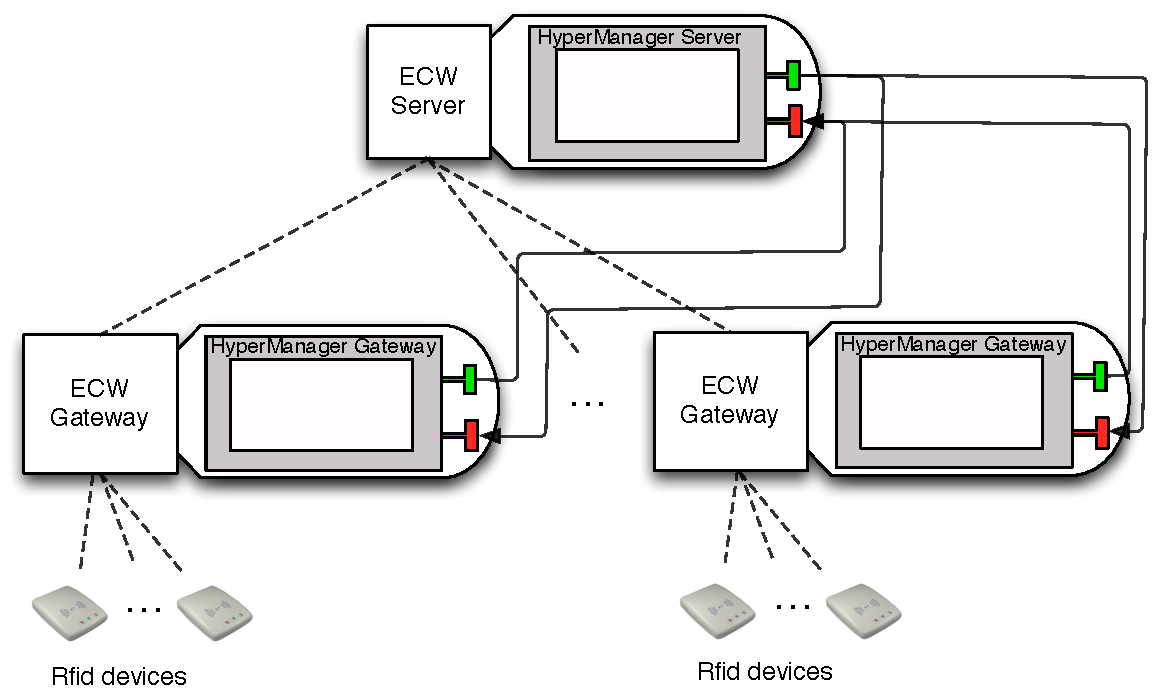
\includegraphics[scale=0.5]{figures/chapter3/architecture.pdf}
		\caption{Hierarchical representation of our case study}		
		\label{fig:hierarchy}
	\end{figure}

		
	Regarding the previously described scenario, this hierarchical view should pose no doubt.
	For each of the \textsc{n} floors of the hotel there are \textsc{m} laundry carts that interact in
	a \textit{one-to-one} style with a gateway.	On the other hand, the gateways communicate 
	with the server on a \textit{n-to-one} style. Moreover, there is also the need to cope for possible 
	maintenance issues. For instance, in the case of malfunction of some device running the \ac{ECW} \textsf{Gateway},
	it may be required to replace it or add a new one in order to avoid any overloading.
	 		 
	  				
	The architecture depicted by Figure \ref{fig:hierarchy}
	also includes \textsc{The HyperManager} application. Indeed, it is deployed alongside	the pre-existent
	distributed system, performing its monitoring on all \textsf{ECW} components. Moreover, the careful reader may notice 
	that the flow of requests go both from the \textsf{HyperManager Server} to
	the \textsf{HyperManager Gateway}, and vice-versa. Indeed, these follow the \textit{pull} and \textit{push}
	styles of communication, respectively. More details regarding these mechanisms will be discussed at a later stage.
	
		
	%%%
	\section[The HyperManager architecture]{The HyperManager architecture}
	\label{sub:thehm}
	
		 \textsc{The HyperManager} is a general purpose monitoring application that was developed 
	in the context of the Spinnaker project. The goal was to deliver a modular
	solution that would be capable of monitoring a distributed application and react to certain events.
	As such, \textsc{The HyperManager} is itself a distributed application, deployed alongside the target 
	application to monitor. %To simplify, we shall consider that this application is constituted by two levels.
	%The upper-level includes one server application, while the lower-level includes several gateways.
		
	Generally, when performing a monitoring task in an application one may consider two types of
	events: \textit{pull} and \textit{push}. The former stands for the usual communication scenario
	where the server regularly \textit{pulls} information from the client. The latter however, 
	is when the client \textit{pushes} data to the server. Both styles
	of communication are employed in \textsc{The HyperManager} application. %Figure \ref{fig:HMServer} depicts
	%the \textit{upper-level} of our \textsc{HyperManager}.
			
	\begin{figure}[H]
		\centering
		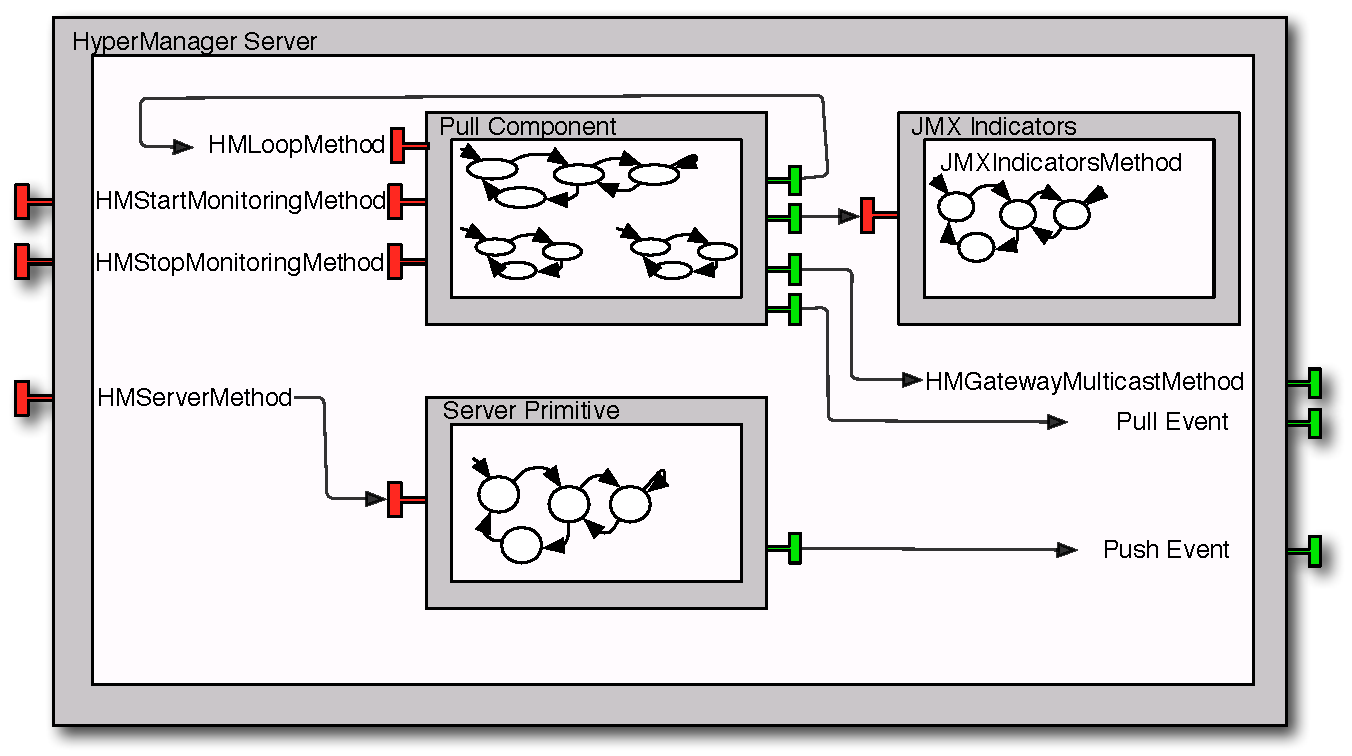
\includegraphics[scale=0.45]{figures/chapter3/HMServer-comp-v2.pdf}
		\caption{HyperManager server component}
		\label{fig:HMServer}		
	\end{figure}	
	
		
	As illustrated by Figure \ref{fig:HMServer}, the \textsf{HyperManager Server} component 
	features three primitive components that are responsible for	 the application logic. Each possesses  
	one or several service methods.
	
	The \textsf{JMX Indicators} component
	features only one service method: it accepts requests about a particular \ac{JMX}\footnote{\ac{JMX} is the standard protocol used for monitoring Java applications.}
	indicator and replies with its status. 
	This encapsulates business code and interacts directly with the \ac{ECW}.
	
	The \textsf{Pull Component} includes three service methods and four client interfaces. As the component's name indicates, it
	is responsible for \textit{pulling} information and emitting it as \textit{pull events}. The service methods \textsf{HMStartMonitoringMethod}
	and \textsf{HMStopMonitoringMethod} are responsible for starting and stopping the \textit{pulling} activity, respectively. Typically, these are the 
	methods called by an administrator. The remaining service method, \textsf{HMLoopMethod}, may pose some doubt. Indeed, it is called from
	one of its own client's interface. Being a \ac{GCM}/ProActive application, it follows the active object paradigm where explicit thread creation is discouraged.
 	As such, making a method \textit{loop} is achieved by making this method send itself a request before concluding its execution.	
 	
 	While in the monitoring loop, the \textsf{HMLoopMethod} method \textit{pulls} information regarding its own local \ac{JMX} indicators and those of its gateways 
 	via a multicast client interface. The last remaining client interface serves the purpose of reporting the \textit{pulled} information as \textit{pull} events.
		
	Last, the \textsf{Server Primitive} component receives \textit{push} information from the \textsf{HyperManager Gateway}s 
	--- typically to alert the occurrence of some anomaly --- and
	emits it as \textit{push} events. %In our implementation both \textit{push} and \textit{pull} events are then displayed
	%in some application with a graphical interface for administration purposes.
		
	The description of the \textsf{HyperManager Gateway} component follow the same spirit. Figure	 \ref{fig:HMGw} depicts its constitution.
	
	
	\begin{figure}[H]
		\centering
		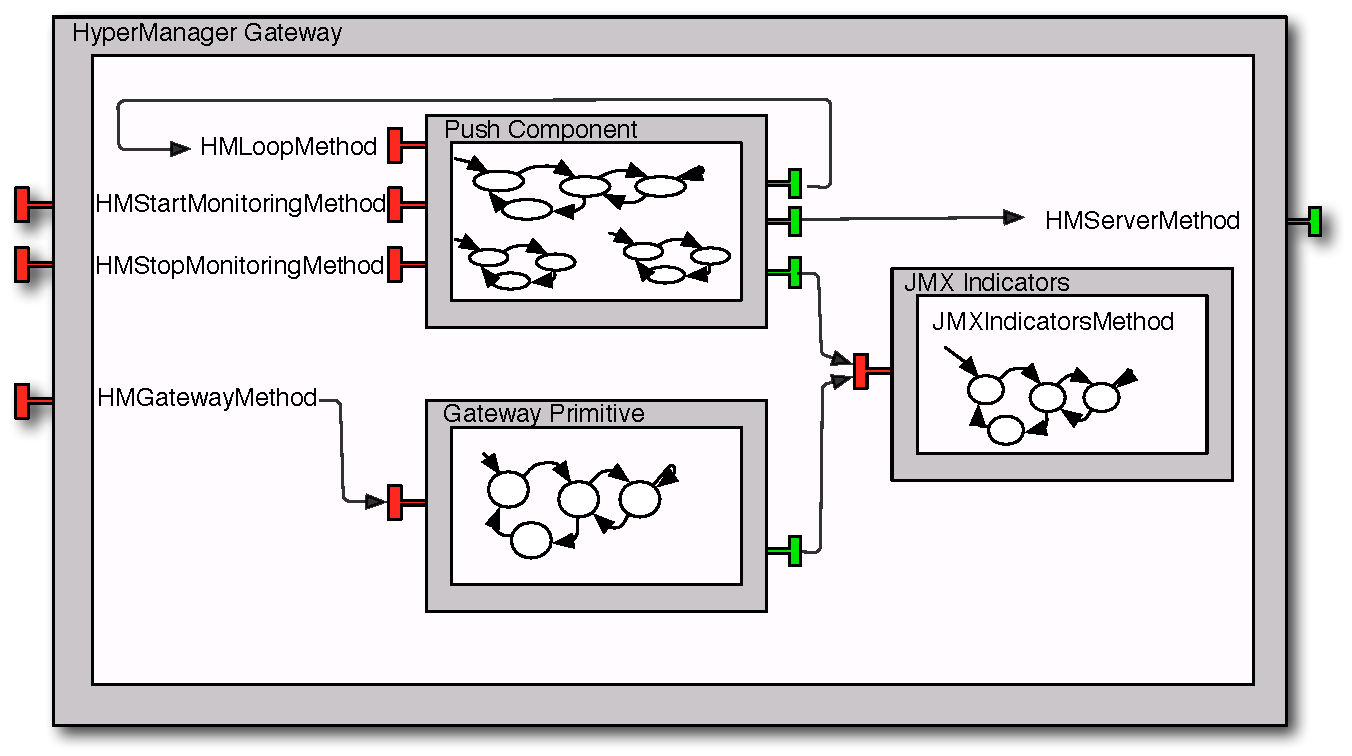
\includegraphics[scale=0.45]{figures/chapter3/HMGateway-comp-v2.pdf}
		\caption{HyperManager gateway component}
		\label{fig:HMGw}		
	\end{figure}		
	
	
	\noindent It is also composed of three primitive components. As expected, the \textsf{JMX Indicators} component has the same semantics as
	described above. 
	
	The \textsf{Push Component} features the same service methods as the \textsf{Pull Component}. Its semantics however, are slightly different.
	While \textit{looping} it will check for the status of its \ac{JMX} indicators, and communicate with  \textsc{The HyperManager} server if some anomaly
	is encountered --- which will then trigger a \textit{push} event.
	
	As for the \textsf{Gateway Primitive} component, its sole purpose is to reply to the \textit{pulling} requests from 
	the \textsf{HyperManager Server} component.
	

\section{Formal specification and verification methodology}		
\label{sec:methodology}		
		
		
			Regarding our modelling and verification \textit{workflow}, the first step is to build 
		the behavioural models by encoding the involved processes in the \textsf{Fiacre} specification 
		language. Naturally, this step can be partially automated as processes such as the \textsf{Queue},
		\textsf{Body}, etc, are computable, i.e., there is an algorithm that generates their behaviour. For instance,
		Listing \ref{lst:queuejmx} depicts the specification of the \textsf{Queue} process for the \textsf{JMX Indicators} 
		component in \textsf{Fiacre}. It should be noted that we need a finite representation of such process: 
		we illustrate this by a \textsf{Queue} bounded at two requests.
		
		
	\lstinputlisting[language=Fiacre,
	                        stepnumber=1, caption=Queue specification of the \textsf{JMX Indicators} component in Fiacre (bounded at two requests), 
	                        label=lst:queuejmx]{listings/chapter3/jmxqueue.tex}		

			
		%enqueuing is correct word	
	\noindent The \textsf{JMX Indicators} component possesses one service method, named
	\textsf{JMXIndicatorsMethod}, taking one argument of \textsf{JMXIndicatorsMethod\_args\_type}
	type. The three labels (lines 1-3) \textsf{Q\_JMXIndicatorsMethod}, \textsf{Serve\_JMXIndicatorsMethod} 
	and \textsf{Error} represent enqueuing of a request to its service method, 
	serving it, and throwing an exception due to exceeding of its capacity, 
	respectively. From \textsf{SEmpty}, upon reception of a request
	the process goes to state \textsf{S1} (lines 11-12), where it can serve the current request
	or receive another one (lines 14-17). The former case leads back 
	to \textsf{SEmpty}. The latter
	takes the execution to \textsf{S11} where it faces the same cases. 
	On the one hand, another request
	will lead to \textsf{SOutOfBounds} (line 21), at which point 
	the action \textsf{Error!errmsg} is emitted since 
	the request queue's maximum capacity is reached 
	--- where \textsf{errmsg} is a variable holding
	information about the antecedent state --- 
	and the execution is transferred to the sink state \textsf{SError} (lines 24-25). 
	On the other hand, since it exhibits a \ac{FIFO} policy, serving a request (line 20) 
	is performed on the initial call by emitting \textsf{Serve\_JMXIndicatorsMethod!a0,a00},
	and performing two assignments: \textsf{a0:=a1} and \textsf{a00:=a11}. The variables
	\textsf{a00}, \textsf{a11}, \textsf{a22} hold the request arguments by order of arrival. Thus, 
	this simple mechanism ensure they are served in an adequate order, i.e., 
	meeting the \ac{FIFO} policy. Moreover, the variables \textsf{a0}, \textsf{a1} and \textsf{a2}
	contain future proxies, and are handled analogously. Naturally, these are implicit --- transparent
	to the programmer ---, but included into the formal model.

		Let us now see how the \textsf{body} process is modelled. As an example, listing \ref{lst:bodyjmx} 
		depicts its specification for the \textsf{JMX Indicators} component.

			\lstinputlisting[language=Fiacre,
	                        stepnumber=1, caption=Body specification of the \textsf{JMX Indicators} component in Fiacre, 
	                        label=lst:bodyjmx]{listings/chapter3/jmxbody.tex}		
		
	
	\noindent Its understanding should pose no doubt. Basically, it idles in state \textsf{s0} until
	\textsf{Serve\_JMXIndicatorsMethod?fid,args} is activated, at which point the execution goes to \textsf{s1} (lines 10-11).
	From \textsf{s1} it emits \textsf{Call\_JMXIndicatorsMethod!fid,args}, therefore starting the actual method
	execution, and moves to \textsf{s11} (lines 13-14). Then, it just waits for the \textsf{JMXIndicatorsMethod} method 
	finish its execution and return, at which point \textsf{R\_JMXIndicatorsMethod?fid,reply} is received, and 
	it goes back to \textsf{s0} (lines 16-17).	
	
		\textsf{Proxy} and \textsf{ProxyManager} processes' behaviour can also be obtained in a systematic 
	manner. Together with the \textsf{Queue} and \textsf{Body} processes they model all the internal
	intricacies of a \ac{GCM} primitive component. The specification of the featured service methods however,
	is of specific nature, and thus a manual task.    
	
	
		Having the Fiacre sources files for all involved processes, we use the \textsc{flac} 
	compiler\footnote{Available online \url{http://gforge.enseeiht.fr/projects/fiacre-compil}} to 
	produce \textsc{Lotos} \cite{Bolognesi:1987:IIS:44211.44214}.
   Then,  we take advantage of the panoply of tools offered by the 
   CADP suite \cite{garavel:inria-00583776} for model generation and formal
   verification by model-checking techniques. Figure \ref{fig:workflow} depicts the overall 
   approach.
          		
	\begin{figure}[H]
		\centering
		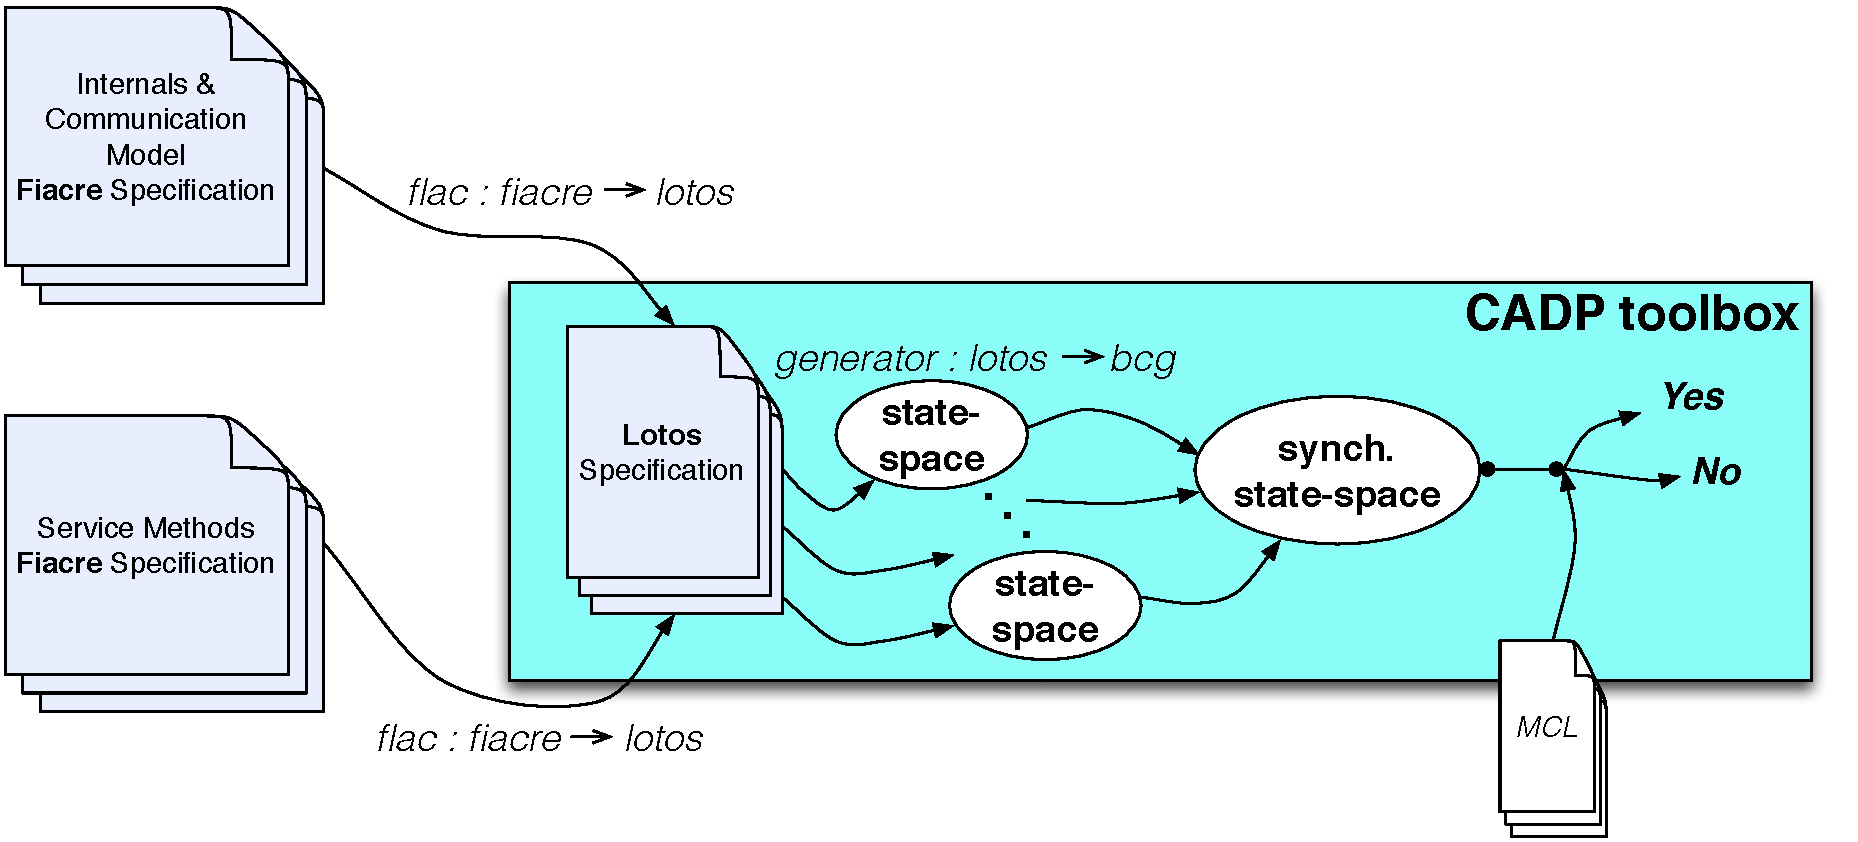
\includegraphics[scale=0.45]{figures/chapter3/mc.pdf}
		\caption{Formal specification and verification workflow}
		\label{fig:workflow}		
	\end{figure}		

	%%%pacagrid ... NEF..
	From CADP, we use \textsf{generator} for state-space generation. This process takes a plaintext
	\textsf{.lotos} file and yields a binary \textsf{.bcg} file encoding a \ac{LTS} that models
	the process behaviour. This file is usually referred to as the state-space. Moreover,
	it should be noted that state-space generation can be performed in a distributed manner.
	CADP's \textsf{distributor} tool implements a distributed algorithm that can be executed on several 
	machines. This can be of great value as	
	each of them is used to generate and store a part of the \ac{LTS}. 
	
		For the purposes of this thesis, we used distributed state-space generation by exploiting
	ProActive \textsf{PACA Grid} --- a computing cloud operated by INRIA, 
	University of Nice, and CNRS-I3S laboratory, and accessible through the 
	ProActive Scheduler\footnote{\url{http://proactive.activeeon.com/index.php?page=proactive_5_min}}.		
	Nevertheless, it should be noted that 	parallel composition through synchronization vectors
	is a sequential process, and thus may be a bottleneck for large systems. Indeed, as we shall see
	later, dealing with large state-spaces was one of the main challenges of this case study.
	
		
	%Typical file management and \ac{LTS} manipulation is conveniently achieved through \ac{SVL} scripts.
	%These encompass commands for state-space generation, label renaming and \ac{LTS} synchronization.
					
    %.exp which describes a network of communicating automata in the EXP 2.0 language defined below
    %svl - Script Verification Language	
				
			 For last, we use \textsf{evaluator4} for model-checking state-spaces against 
    \ac{MCL} \cite{Mateescu:2008:MCL:1423684.1423700} formulas --- an extension of the
    alternation-free regular $\mu$-calculus \cite{WinskellMuCalc} with facilities for manipulating data.		

		In the following, to optimize the size of the model, composite components have no request queue and 
	requests are directly forwarded to the
    targeted primitive component. This has no influence in the system's semantics as the request queues of the primitive components are sufficient for dealing with asynchrony and requests from the subcomponents are directly 
    dispatched too. We set the primitive components 
    with re-entrant calls --- \textsf{Pull Component} and \textsf{Push Component} --- with a \textsf{queue} 
    of size 2, and the remaining from the \textsf{HyperManager Server}  
    and \textsf{HyperManager Gateway} composites with size 1 and 2, respectively. Furthermore,
	we set the future proxy domain to range over \{0..1\}, and consider the existence of
    two \ac{RFID} devices per gateway.

\section{The HyperManager as a formal methods case study}
\label{sec:spec}

		
		As mentioned above, \textsc{The HyperManager} is a \ac{GCM}/ProActive application. A natural
	choice for its behavioural specification is therefore pNets. This task requires the specification
	of all service methods composing the application. These transparently interact with
	the component's internal intricacies --- component queue, proxy manager, ... ---, 
	that are also included in the model.
	
		In the following we dedicate Subsection \ref{sub:hmgwverif},
		Subsection \ref{sub:hmserververif}, and Subsection \ref{sub:prod1} to the discussion
		on the specification and verification by model-checking of the \textsf{HyperManager Gateway} component,
		\textsf{HyperManager Server} component, and overall system product, respectively.
		Next, Section \ref{sec:reconfig} deals with the inclusion of structural reconfigurations
		in our model. Section \ref{sec:hyperremarks} gives some final
		remarks regarding this case study.
	
		Moreover, for more material on this case study --- namely the specification's source files ---,
		the reader is invited to check its companion 
		website\footnote{\url{http://www-sop.inria.fr/members/Nuno.Gaspar/HyperManager.php}}.	
	
	  

    

\subsection{On HyperManager Gateway}
\label{sub:hmgwverif}


\subsubsection{\textsf{JMX Indicators} component}	

	As seen above, the \textsf{JMX Indicators} primitive component only features one service method, 
	\textsf{JMXIndicatorsMethod}, with \textsf{JMXIndicatorsMethod\_args\_type} and 
	\textsf{JMXIndicatorsMethod\_return\_type} as argument and return types, respectively. These
	are specified as shown by Listing \ref{lst:typesjmx}.

			\lstinputlisting[language=Fiacretypes,
	                        stepnumber=1, caption=Specification for the \textsf{JMXIndicatorsMethod} argument and return types, 
	                        label=lst:typesjmx]{listings/chapter3/jmxtypes.tex}	


	\noindent For the sake of simplicity, we only model two 
	types of \ac{JMX} indicators: \textsf{MemoryUsage} and \textsf{DeviceStatus}. The latter takes into account an identifier, 
	returning its availability status. This relates to the status of a \ac{RFID} reader transmitting to the \ac{ECW} Gateway.
	While the former accounts for the stability status of the memory. 
	
	%JMX no servidor nao tem isso... contextual stuff: synch. with a context that only sends memory status requests
	%compositional

	Listing \ref{lst:mjmx} illustrates the specification of the \textsf{JMXIndicatorsMethod} method behaviour.
	
		\lstinputlisting[language=Fiacre,
	                        stepnumber=1, caption=\textsf{JMXIndicatorsMethod} specification, 
	                        label=lst:mjmx]{listings/chapter3/jmxm.tex}		
	
	
	\noindent Basically, it waits at the \textsf{s\_init} state until it receives a request call regarding
	one of the \ac{JMX} indicators (lines 11-13). Then, it goes to state \textsf{s\_mem} or
	\textsf{s\_dev}, depending on which \ac{JMX} indicator is queried:
	a request to the memory usage takes the execution
	to the former, while a request to the device statuses takes the execution to the latter.
	From \textsf{s\_mem} it randomly replies one of the possible values for
	the memory usage and goes back to \textsf{s\_init} (lines 16-19). As expected, the 
	same behaviour w.r.t. device statuses occurs from \textsf{s\_dev} (lines 21-22).
	The careful reader may wonder about	the rather different specification approaches
	between the reply of the two \ac{JMX} indicators. Indeed, for the memory usage it 
	exhaustively lists all possible reply values, and emits a non-deterministic choice among them.
	For the devices statuses however, it simply replies with a non-instantiated variable \textbf{x},
	that does the work of ranging over all possible reply values. Naturally, both approaches have 
	the same semantics, it is merely a matter of style.
	
	
	The Fiacre specification language allows for fairly simple and intuitive descriptions of 
	automata-based models. Nevertheless, a more convenient representation for 
	illustrating automata is in its graphical form. For instance, Figure \ref{fig:JMX} depicts 	
	the behaviour of the \textsf{JMXIndicatorsMethod} method.	
	
	\begin{figure}[H]
		 \centering
		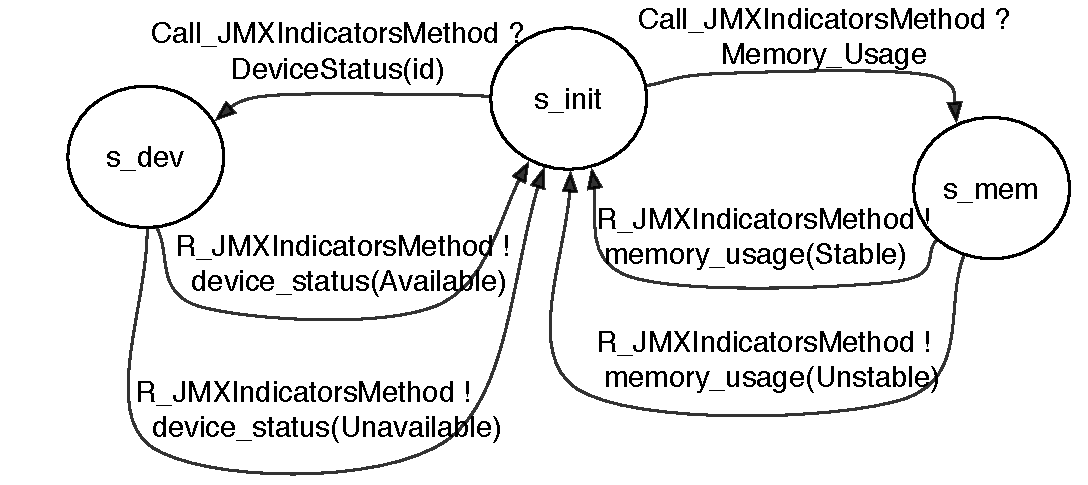
\includegraphics[scale=0.6]{figures/chapter3/JMXIndicatorsMethod.pdf}
		\caption{Behaviour of the JMXIndicatorsMethod method}
		\label{fig:JMX}		
	\end{figure}			
	
		
	\noindent Its understanding is straightforward, as it closely follows Fiacre's specification
	from Listing \ref{lst:mjmx}. There is, however, one	 small nuance: it does not include the 
	future proxies. Indeed, these are related to the internal machinery of 
	\ac{GCM} components, and one would rather avoid such intricacies when specifying service
	methods. As such, they are omitted in the graphical representations: we consider these representations
	as an \textit{user-version} \ac{LTS}, i.e., typically what a user would specify without paying 
	attention to the future proxies mechanism. 
			

\subsubsection{\textsf{Gateway Primitive} component}	
	
	Let us now look at the behaviour of the \textsf{HMGatewayMethod} method. Listing
	\ref{lst:mgw} details its specification in Fiacre.		
	
	\lstinputlisting[language=Fiacre,
	                        stepnumber=1, caption=\textsf{HMGatewayMethod} specification, 
	                        label=lst:mgw]{listings/chapter3/gwm.tex}		
			
	\noindent Despite its apparatus, this service method offered by the \textsf{Gateway Primitive} component 
	has also a fairly simple semantics. It acts merely as a request forwarder for the \textsf{JMX Indicators} component.
	A far more convenient specification is given by Figure \ref{fig:GwM}.	
	     
	\begin{figure}[H]
		 \centering
		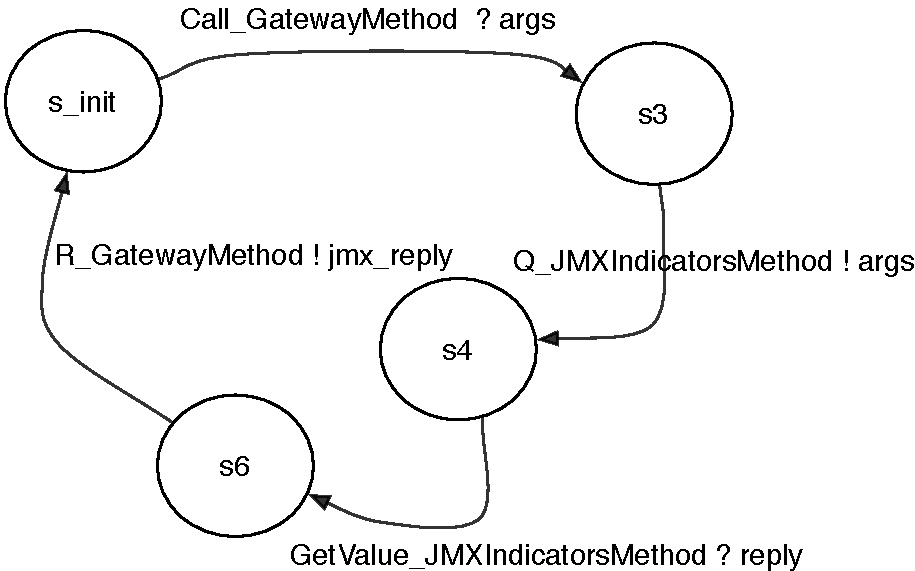
\includegraphics[scale=0.6]{figures/chapter3/HMGatewayMethod.pdf}
		\caption{Behaviour of the HMGatewayMethod method}
		\label{fig:GwM}		
	\end{figure}		

	
	\noindent For this example the extra verbosity introduced by the handling of future proxies is even
	more evident. Indeed, all this machinery ends up obfuscating the method's actual behaviour.		
	In the following, we constrain ourselves to the \textit{user-version} \ac{LTS} representation for 
	the description of service method behaviour. Hopefully, this shall facilitate the understanding
	of the remaining specifications.		


\subsubsection{\textsf{Push Component} component}	
	
	
	Regarding the \textsf{Push Component}, it is composed by three service methods:  \textsf{HMStartMonitoringMethod},
	\textsf{HMStopMonitoringMethod} and \textsf{HMLoopMethod}. Further, the global variable \textbf{started} is shared
	among them. For the sake of clarity communication actions are 
	written in black, while \textit{local} computations (e.g. guard evaluations, assignments) are written in blue. 
	Their intended meaning should pose no doubt.
	
	   \begin{figure}%[H]
	\centering
	\begin{minipage}[b]{0.45\linewidth} 
	\centering
	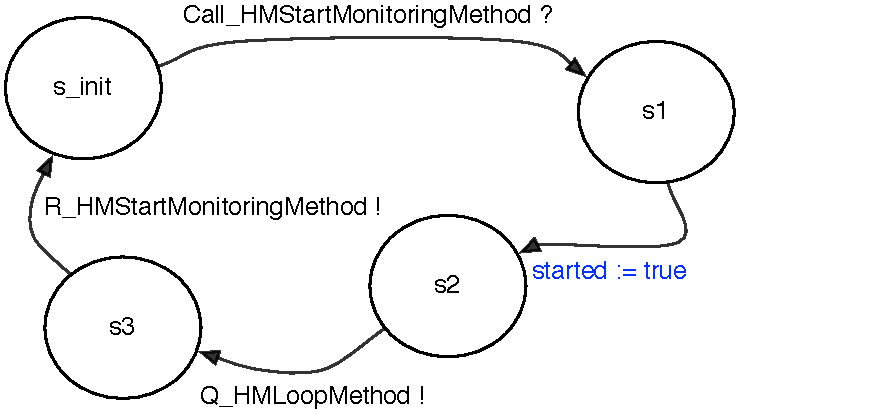
\includegraphics[width=\textwidth]{figures/chapter3/HMStartMethod.pdf}
	\caption{Behaviour of the HMStartMonitoringMethod method}
	\label{fig:start}
	\end{minipage}
	\hspace{0.10cm}
	\begin{minipage}[b]{0.45\linewidth} 
	\centering
	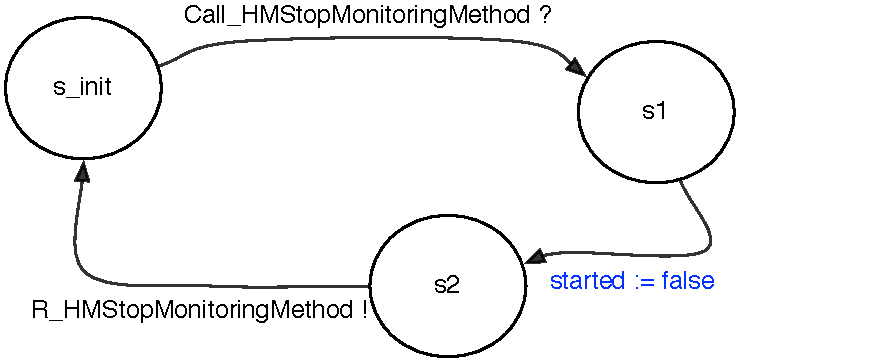
\includegraphics[width=\textwidth]{figures/chapter3/HMStopMethod.pdf}
	\caption{Behaviour of the HMStopMonitoringMethod method}
	\label{fig:stop}
	\end{minipage}
	\end{figure}	  
		
	Figure \ref{fig:start} and Figure \ref{fig:stop} depict the behaviours of the \textsf{HMStartMonitoringMethod} and 
	\textsf{HMStopMonitoringMethod} methods, respectively. Basically, they are responsible for	
	enabling/disabling the \textit{looping} process of the \textsf{HMLoopMethod}. This is achieved 
	by the shared variable \textbf{started}. On the one hand, invoking \textsf{HMStartMonitoringMethod} sets \textbf{started} 
	to \textit{true} and performs an invocation to \textsf{HMLoopMethod}. On the other hand, 
    \textsf{HMStopMonitoringMethod} sets \textbf{started} to \textit{false}. 

	It should be noted that these local computations involving the global variable \textbf{started} are
	merely syntactic sugar for the emission and reception of messages to another process. In practice, 
	the involved labels  are \textsf{GuardQuery}, \textsf{GuardReply?b:bool}, \textsf{SetFalse} and \textsf{SetTrue}.
	Their meaning should be obvious from their labels.
		
	The last remaining service method	to describe is the most interesting one --- the \textsf{HMLoopMethod} 
	method. Its behaviour is depicted by Figure  \ref{fig:LG}. 
	
\begin{figure}%[H]
	\centering
		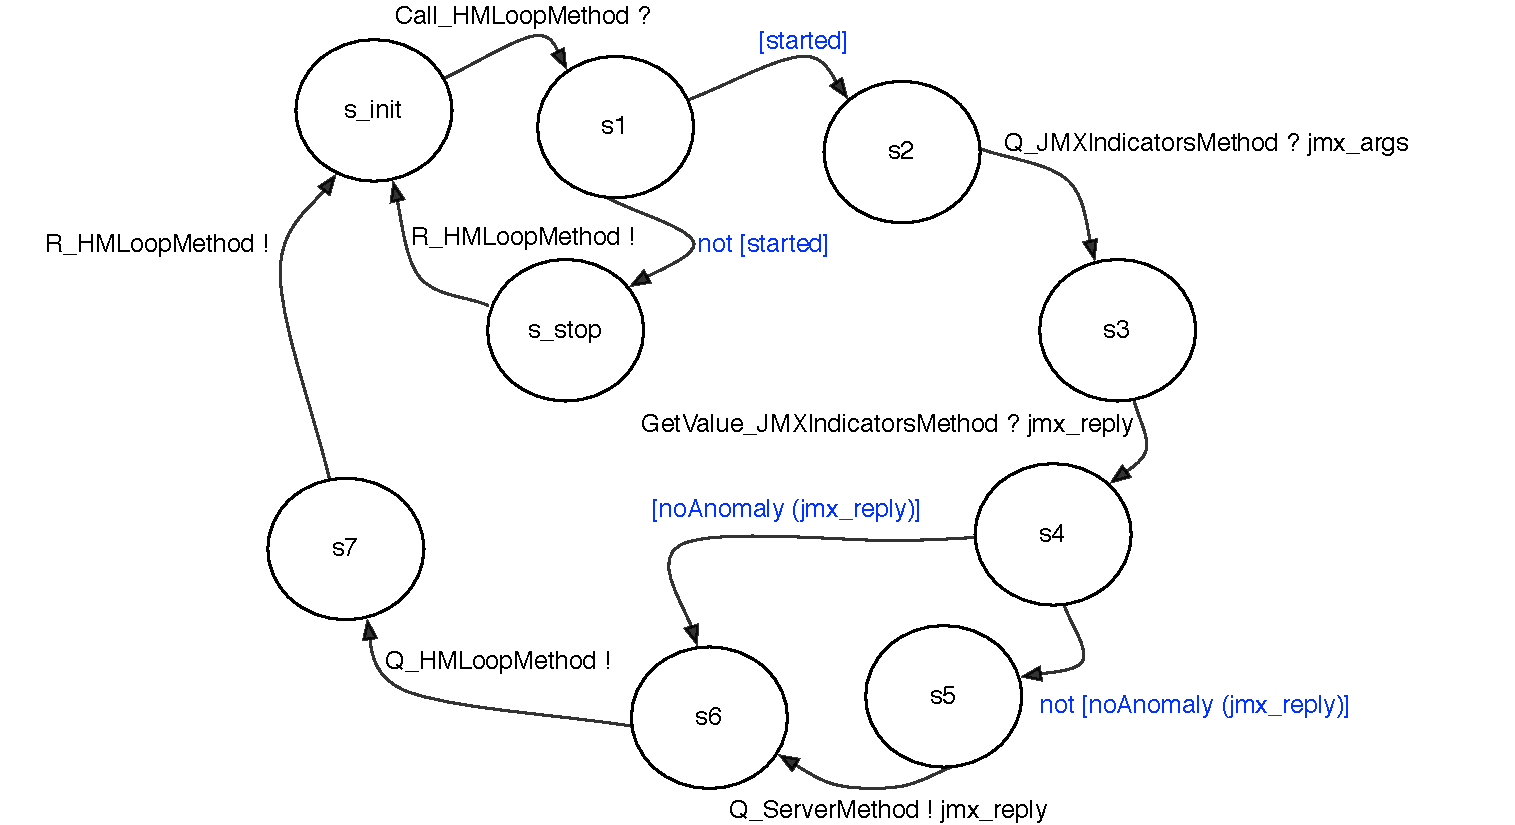
\includegraphics[scale=0.5]{figures/chapter3/HMLoopMethodatGateway.pdf}
		\caption{Behaviour of the HMLoopMethod method for the HyperManager Gateway}
		\label{fig:LG}		
\end{figure}	
	
	\noindent The reception of \textsf{Call\_HMLoopMethod} action starts the method execution, 
    moving from state \textsf{s\_init} to state \textsf{s1}. Then, the global variable \textbf{started} is checked.
    If it evaluates to \textit{false} the method returns by emitting a \textsf{R\_HMLoopMethod}
    message. Otherwise, the execution proceeds by querying the gateway's local \ac{JMX} indicators 
    --- from \textsf{s2} to \textsf{s3} through \textsf{Q\_JMXIndicatorsMethod?jmx\_args}. The reply
    is received by \textsf{GetValue\_JMXIndicatorsMethod?jmx\_reply} and evaluated at state \textsf{s4}.
	If an anomaly is detected (e.g. unstable memory), it is reported to the \textsf{HyperManager Server} component
	through the message \textsf{Q\_ServerMethod!jmx\_reply}, thus 
	moving from state \textsf{s5} to state \textsf{s6}. If no anomaly is found, the execution proceeds directly
	to state \textsf{s6}, where a call to the method itself is performed: \textsf{Q\_HMLoopMethod}. This places
	a request on the \textsf{Push Component} component queue --- thus making the method \textit{loop} --- and
	transfers the execution to state \textsf{s7}. It should be noted that this request is scheduled as any other 
	one: the \ac{FIFO} policy dictates that requests are served by order of arrival, and therefore a potential
	 \textsf{Q\_HMStopMonitoringMethod} enqueued in the meantime would be served before this new 
	 \textsf{Q\_HMLoopMethod} request.        
	Finally, from state \textsf{s7}, the message \textsf{R\_HMLoopMethod} is emitted, and the method execution
	concludes by going back to state \textsf{s\_init}.
  


\subsubsection{Model Generation and Proven Properties}
		
		Model generation is performed by synchronizing all the involved processes --- 
		\ac{GCM} internals and service methods --- of the \textsf{HyperManager Gateway} component.		
		Table \ref{tab:modelG} illustrates its state-space information. 		

\begin{table}[H]
\begin{center}
\begin{tabular}{| l | c | c | c | c |}
\hline
                             &  \textbf{States} & \textbf{Transitions} & \textbf{File Size} \\
\hline
   \textsf{hmgateway.bcg}            &  14.931.628  &  147.485.103  &  $\sim$ 295 mb\\
  \hline
\end{tabular}
\end{center}
\caption{State-space information for the \textsf{HyperManager Gateway} component}
\label{tab:modelG}
\end{table}

	  
	Having the state-space generated we can now prove some properties regarding the expected behaviour of the model.
	Specifying properties of interest in \ac{MCL} is a rather intuitive task due to its expressiveness and conciseness. 
	Its main ingredients include patterns extracting data values from \ac{LTS} actions,
	modalities on transition sequences described using extended regular expressions, 
	and programming language constructs.
	
	For instance, one could  wonder about this rather unusual \textit{looping} mechanism. Once 
	setting the global variable \textsf{started} to \textit{true} 
	--- accomplished by \textsf{Q\_HMStartMonitoringMethod} ---, the \textit{looping} continues until a 
	request to stop monitoring is received. That is, there is no execution path in 
	which the global variable \textbf{started} evaluates to \textit{false} without the occurrence of 
	a \textsf{Q\_HMStopMonitoringMethod}.	 Property \ref{prop:loopsgw} encodes this statement in \ac{MCL}.


%loop-while-flag-true
\begin{property}[loops while variable started is true]
\label{prop:loopsgw}
\begin{verbatim}
	
	[ "Q_HMStartMonitoringMethod" . 
	     (not "Q_HMStopMonitoringMethod")* . "GuardReply !FALSE" ] false
\end{verbatim}
\end{property}%2m48s


	\noindent More precisely, Property \ref{prop:loopsgw} reads: all paths starting with the label \textsf{Q\_HMStartMonitoringMethod},
	followed by any other sequence of labels not including \textsf{Q\_HMStopMonitoringMethod}, and
	ending by \textsf{GuardReply !FALSE}, cannot occur. Model-checking \textsf{hmgateway.bcg}  against this formula
	demonstrates that it is indeed true.
	

	Another property of interest concerns the overloading of the \textsf{HyperManager Server} component
	with unnecessary messages. We want to ensure that we cannot
	\textit{push} data if not in the presence of an anomaly. This is modelled by Property \ref{prop:overload}.

\begin{property}[no server overload]
\label{prop:overload}

 \begin{verbatim}
 
[ ((not "R_JMXIndicatorsMethod !memory_usage (Unstable)")* . 
       "Q_ServerMethod.*")  |
  ((not "R_JMXIndicatorsMethod !device_status ((Unavailable, IdTwo))")* . 
       "Q_ServerMethod.*") |
  ((not "R_JMXIndicatorsMethod !device_status ((Unavailable, IdOne))")* . 
       "Q_ServerMethod.*") 
] false
 \end{verbatim}
  \end{property}


	\noindent The above \ac{MCL} formula states that all paths starting with any sequence of labels
	not including the reply of an anomalous \ac{JMX} indicator --- \textsf{R\_JMXIndicatorsMethod !memory\_usage (Unstable)},
	\textsf{R\_JMXIndicatorsMethod !device\_status ((Unavailable, IdTwo))} and 
	\textsf{R\_JMXIndicatorsMethod !device\_status ((Unavailable, IdOne)} ---, followed by
	a \textsf{Q\_ServerMethod.*} --- where * is a \textit{wildcard} matching all possible arguments ---, cannot occur.	
	With no surprise, Property \ref{prop:overload} is also proved to be satisfied by the model.


\subsection{On HyperManager Server}
\label{sub:hmserververif}
	
	
\subsubsection{\textsf{JMX Indicators} component}		
	
		As seen for the \textsf{HyperManager Gateway} component, the \textsf{HyperManager Server} component also features 
	a 	\textsf{JMX Indicators} component.	This one however, is not endowed with \ac{JMX} indicators
	for the \ac{RFID} devices statuses. 
	
		Technically, we attach to the \ac{LTS} modelling the behaviour of the \textsf{JMX Indicators}
		component (see Figure \ref{fig:JMX})
	a context that constraints its requests. This is achieved by synchronization with another \ac{LTS}
	that solely emits requests regarding the memory status. This approach for contextual state-space 
	generation is compositional and thus promotes reusability. 
		

\subsubsection{\textsf{Server Primitive} component}		

   As seen above, upon detection of an anomaly, the \textsf{HyperManager Gateway} components \textit{push} 
   the relevant information to the \textsf{HyperManager Server}. Then, it is emitted as a
  \textit{push} event. This behaviour is depicted by Figure \ref{fig:SM}. 
  
	\begin{figure}[H]
		\centering
		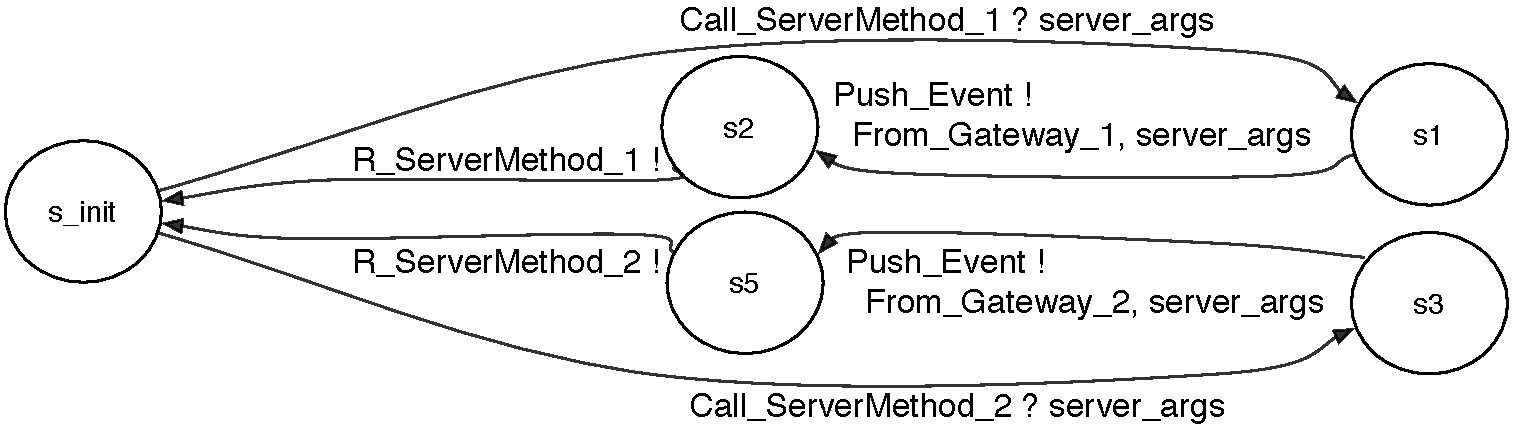
\includegraphics[scale=0.5]{figures/chapter3/HMServerMethod.pdf}
		\caption{Behaviour of the HMServerMethod method}
		\label{fig:SM}		
	\end{figure}	  
  
  \noindent The careful reader will notice that the emitted event also contains
   the information regarding the \textsf{HyperManager Gateway} component from which 
   the anomaly originated. This should come as no surprise as there can be
   several of them, and properly identifying the source of an abnormal situation 
   is of paramount importance. In our model, we consider the existence of two 
   \ac{ECW}/HyperManager gateways, and therefore we include specific labels
   --- \textsf{Call\_ServerMethod\_i}$_{i\in\{1,2\}}$ and  \textsf{R\_ServerMethod\_i}$_{i\in\{1,2\}}$ --- 
	for  communicating with them.
  
  
\subsubsection{\textsf{Pull Component} component}		  
  		
	
	The \textsf{Pull Component} component is composed by three service methods: \textsf{HMStartMonitoringMethod},
	\textsf{HMStopMonitoringMethod}, and \textsf{HMLoopMethod}. Indeed, these have the same names as the service methods
	for the \textsf{Push Component} component. In fact, their \textsf{HMStartMonitoringMethod} and 
	\textsf{HMStopMonitoringMethod} methods possess the same semantics (depicted by Figure \ref{fig:start} 
	and Figure \ref{fig:stop}). Their \textsf{HMLoopMethod} method however, behave differently.
    Figure \ref{fig:LS} depicts its behaviour for the \textsf{Pull Component}.

	\begin{figure}[H]
	\centering
		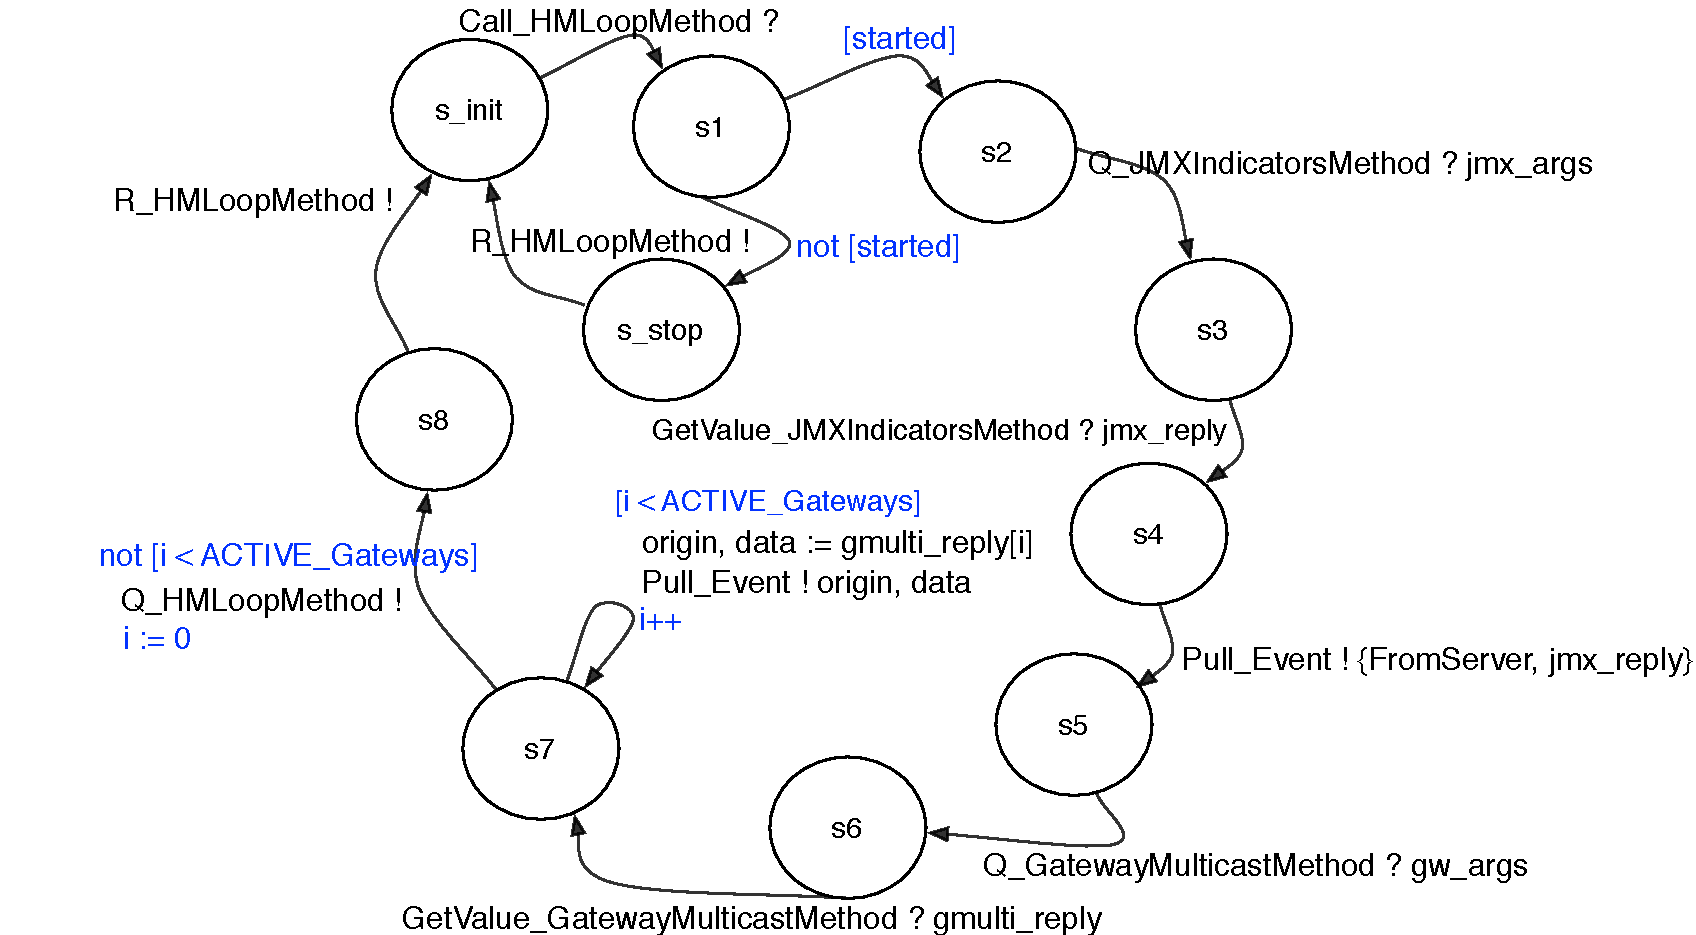
\includegraphics[scale=0.5]{figures/chapter3/HMLoopMethodatServer2.pdf}
		\caption{Behaviour of the HMLoopMethod method for the HyperManager Server}
		\label{fig:LS}		
	\end{figure}	  

	\noindent Its \textit{looping} mechanism is also handled through a shared 
	variable named \textbf{started}.  While \textit{looping}, 
	the local \ac{JMX} indicators are queried, and its reply emitted 
	as \textit{pull} events. Moreover, through the multicast interface 
	the monitoring information is \textit{pulled} from the bound gateways. 
	This, emits as many \textit{pull}
    events as the number of bound gateways. Last, a request to 
    itself is performed in order to continue \textit{looping}.


\subsubsection{Model Generation and Proven Properties}


	Table \ref{tab:modelS} illustrates the relevant information concerning \textsf{HyperManager Server}'s 
	state-space.

\begin{table}[H]
\begin{center}
\begin{tabular}{| l | c | c | c | c |}
\hline
                             &  \textbf{States} & \textbf{Transitions} & \textbf{File Size} \\
\hline
  \textsf{hmserver.bcg}                                   &   12.787.376   &  187.589.422  &  $\sim$  363 mb\\
  %\textsf{hmserver-min.bcg}    &   12.787.376  &   187.589.422 &   $\sim$  396 mb \\
  \hline
\end{tabular}
\end{center}
\caption{State-space information for the \textsf{HyperManager Server} component}
\label{tab:modelS}
\end{table}

		
	It should be noted that we can also prove properties regarding the \ac{GCM} internals.
	For instance, a rather trivial property we can expect to hold is that we can reach a state 
	which exceeds the maximum capacity of the request queue. 
	For the \textsf{Server Primitive} component, this can be modelled in \textsf{MCL} as demonstrated
	by Property \ref{prop:queueex}
  	
	\begin{property}[reachable exception]
	\label{prop:queueex}
	\begin{verbatim}
	
		< true* . 'QueueException_ServerPrimitive !.*'> true
	\end{verbatim}
	\end{property}

	\noindent Formally, this property reads: from any state, there exists an execution path that can encompass the label
	\textsf{QueueException\_ServerPrimitive !.*}. As expected, this property is proved to be satisfied by the model.
	
		Another property regarding the \ac{GCM} internals concerns the use of proxies. For instance,
	the \textsf{HMLoopMethod} needs to request
	a proxy in order to be able to invoke the service method from the \textsf{JMX Indicators} component. 
	This is encoded as demonstrated by Property \ref{prop:proxy}.
	
	 \begin{property}[need for proxy]
	\label{prop:proxy}	 
	 
	\begin{verbatim}
	
		[ (not "GetProxy_JMXIndicatorsMethod.*")* . 
		             "Q_JMXIndicatorsMethod.*"] false
	\end{verbatim}
   \end{property}
	%proved true. job #3128 (proxy_request2.mcl)
	%2h 24m
   
   \noindent Formally, the above property reads: all execution paths starting with any sequence of labels not including
   \textsf{GetProxy\_JMXIndicatorsMethod.*}, and followed by \textsf{Q\_JMXIndicatorsMethod.*}, cannot occur.
    With no surprise, model-checking this property confirms that it is satisfied by the model.
	    
\subsection{On System Product}
\label{sub:prod1}

	%- space state explosion phenomena
   %- action communication hiding
 
 	%We generated the product of our system	with 2 gateways. Table \ref{tab:modelSP} shows the relevant information.
 	
	We attempted to generate a system product constituted by two \textsf{HyperManager Gateway}s and 
	one \textsf{HyperManager Server} components. However, even on a machine with 90 GB of RAM, we experienced
	the so common state-space explosion phenomena. Indeed, as discussed in Section \ref{sec:methodology},
	while we can use distributed state-space generation, and thus spread the workload among several machines,
	synchronizations products remain a sequential task. 
	
	This arises often in the analysis of complex systems. To this end, \textit{communication hiding} 	
	comes as an efficient and pragmatic approach for tackling this issue. Indeed, it allows the specification of 
	actions that need not to be observed for verification purposes, thus yielding
	more tractable state-spaces.
	
	Table \ref{tab:modelSP} illustrates the effects of applying this technique to the model. The sole
	\textit{communication actions} being hidden are the ones involved in (1) the request transmission
	from the \textsf{Queue} to the adequate method --- \textsf{Serve\_} and \textsf{Call\_} ---, 
	(2) the proxy machinery ---\textsf{GetProxy\_}, \textsf{New\_} and \textsf{Recycle\_} ---, 
	and (3) finally in the \textit{guard} of the \textit{looping} methods --- \textsf{GuardQuery},
	\textsf{GuardReply}, \textsf{SetFalse} and \textsf{SetTrue}. 
	

\begin{table}[H]
\begin{center}
\begin{tabular}{| l | c | c | c |}
\hline
                             &  \textbf{States} & \textbf{Transitions} & \textbf{File Size} \\
\hline
   \textsf{hmgateway-hidden.bcg}           & 14.931.628  & 147.485.103  &  $\sim$  287 mb\\
   \textsf{hmgateway-hidden-min.bcg}   &   409.374      & 4.007.232     &  $\sim$  8.5 mb\\
  \hline
   \textsf{hmserver-hidden.bcg}           &  12.787.376    & 187.589.422    &   $\sim$  375 mb\\
  \textsf{hmserver-hidden-min.bcg}   &      5.761.504 &  85.157.420   &   $\sim$  179 mb \\
  \hline
  \textsf{SystemProduct.bcg}                                &  342.047.684  & 3.026.114.393 &  $\sim$  5.27 gb\\
  \textsf{SystemProduct-min.bcg}   &  259.340.044  &  2.396.896.830  &  $\sim$  4.83 gb\\
 \hline
\end{tabular}
\end{center}
\caption{State-space information for the overall system product}
\label{tab:modelSP}
\end{table}

		The lines suffixed by \textsf{-hidden} indicate the results obtained by \textit{hiding}
		the mentioned \textit{communication actions} in the \textsf{HyperManager Gateway}
		and \textsf{HyperManager server} state-spaces. For both, no effect is noticed on the 
		size of the \ac{LTS}. However,
		there is a decrease in the file size. This is due to the fact that the \textit{hiding} process
		yields several $\tau$-transitions, which facilitates file compression. More importantly, this 
		has the consequence of leveraging the subsequent \textit{minimization} process:
		the entries suffixed by \textsf{-min} mean that minimization by branching \textit{bisimulation} 
		was applied.	 Indeed, we even obtain a reduction by two orders of magnitude (!) for the 
		\textsf{HyperManager Gateway} state-space. 
		
			%With
		
		\textsc{The HyperManager} comes as a monitoring application that should be able to properly
		trace the origin of an anomaly. As such, one behavioural property that we expect to hold is that
		whenever an abnormal situation is detected by a \textsf{HyperManager Gateway}, it is \textit{fairly inevitable} 
		to be reported as a \textit{push event} that correctly identifies its origin. 
		
		First, we shall use \ac{MCL}'s macro capabilities to help us build the formula:
		
		%\scalebox{0.5}{

		\begin{verbatim}
			macro GETVALUE_1_MEMORY () = 
			  "GetValue_JMXIndicatorsMethod_Push_1 !memory_usage (Unstable)" 
end_macro

macro PUSH_1_MEMORY ()     = 
  ("Push_Event (FirstGateway, UnstableMemoryUsage)")  
end_macro
...
		\end{verbatim} 

		
		\noindent The above macros should be self-explanatory. The former represents the detection of an anomaly
		coming from the first \textsf{HyperManager Gateway} --- the model is instantiated with two \textsf{HyperManager Gateway}s,
		thus we differentiate  their actions by suffixing them adequately. The latter stands for the emission
		of the \textit{push} event corresponding to that anomaly. The macros for the remaining
		relevant actions are defined analogously.
		
			Moreover, we define the following macro generically encoding the 
			\textit{fair inevitability}\footnote{We consider the definition by 
			Queille and Sifakis \cite{journals/acta/QueilleS83}: a sequence is fair iff it does not infinitely often 
			enable the reachability of a certain state without infinitely often reaching it.} that
			after an \textit{anomaly} the system emits a \textit{push}.
			
		\begin{verbatim}
			macro FAIRLY_INEVITABLY_A_PUSH (ANOMALY, PUSH) =
       [ true* . "ANOMALY" . (not "PUSH")* ]
           < (not PUSH)* . PUSH > true
end_macro
		\end{verbatim}		
		
		
		\noindent Having the macros defined, we can now write the formula of interest:


		\begin{property}[push fairly inevitable] 
		\label{prop:fair1}
			\begin{verbatim}	
			
(FAIRLY_INEVITABLY_A_PUSH(GETVALUE_1_MEMORY, PUSH_1_MEMORY) and
 FAIRLY_INEVITABLY_A_PUSH(GETVALUE_2_MEMORY, PUSH_2_MEMORY) and
 FAIRLY_INEVITABLY_A_PUSH(GETVALUE_1_DEVICE_1, PUSH_1_DEVICE_1) and
 FAIRLY_INEVITABLY_A_PUSH(GETVALUE_1_DEVICE_2, PUSH_1_DEVICE_2) and
 FAIRLY_INEVITABLY_A_PUSH(GETVALUE_2_DEVICE_1, PUSH_2_DEVICE_1) and
 FAIRLY_INEVITABLY_A_PUSH(GETVALUE_2_DEVICE_2, PUSH_2_DEVICE_2)
)\end{verbatim}
\end{property}		

		%job #3070, 8h 9m		
		
		\noindent Basically, property \ref{prop:fair1} states that it is fairly inevitable that
		the appropriate push event is triggered after the detection of an anomaly.
		As expected, it is satisfied by the model.
		
		
				 %(fair) inevitability 
			%	\begin{property}
			%	\begin{verbatim}
			%		[ true* . ("GETVALUE_JMXINDICATORSMETHOD_PushComponent_1 !POS (1) !DEVICE_STATUS (DEVICE_AVAILABILITY_TYPE (UNAVAILABLE, IDTWO))	") . 
			%		             (not "PUSH_EVENT !PUSH_EVENT (UNAVAILABLEDEVICE (IDTWO), FIRSTGATEWAY)") ] 
			%		< (not "PUSH_EVENT !PUSH_EVENT (UNAVAILABLEDEVICE (IDTWO), FIRSTGATEWAY)")* .
			%		    ("PUSH_EVENT !PUSH_EVENT (UNAVAILABLEDEVICE (IDTWO), FIRSTGATEWAY)") > true
			%	\end{verbatim}
			%	\end{property}
				%it is true. job #2652, 2h23min
				%TODO: prove that thing in the general sense...
		
	%[ true* . "SEND" . (not "RECV")* ]
    %< (not "RECV")* . "RECV" > true
       
		 %The above property accounts for the \textit{push} events. Another property of interest relates the request for        
        
        

\section{The case study reloaded: on structural reconfigurations}
\label{sec:reconfig}


	As seen so far, \thehm\ acts as a monitoring application with two styles of
	communication: \textit{pull} and \textit{push}. However, it also needs to cope with structural 
	reconfigurations. This means that at runtime the architecture of the application can evolve
	by, say, establishing new bindings and/or removing existing ones.
		
	For \ac{GCM} applications \textit{bind} and \textit{unbind} operations are handled by the component
	owning the \textit{client} interface that is supposed to be reconfigurable. This should come
	as no surprise, indeed, it follows the same spirit as in object-oriented languages: an object
	holds the reference to a target object; it is this object that must change the reference it holds.
	
	In our case study, these reconfigurations can occur both from the \textsf{HyperManager Server} 
	 --- when \textit{pulling} data from the bound gateways ---, and from a \textsf{HyperManager Gateway}
	 --- when \textit{pushing} data to the server.
	The difference lies in the fact that the \textsf{HyperManager Server} communicates via a \textit{multicast} interface, 
	unlike the \textsf{HyperManager Gateway}s that establish standard \textit{1-to-1} 
	communications. %Therefore, these are dealt in a different manner. 
	
\subsection{On HyperManager Reconfigurable Gateway}
\label{sub:hmrgwverif}	
	
			
	  In Subsection \ref{sub:reconfig}, we showed how a reconfigurable client interface is modelled
	  in pNets. In particular, Figure \ref{fig:bc} detailed all the internal machinery for singleton interfaces.			
	  For this case study, in practice, to the 
	  \textsf{HyperManager Gateway} model discussed in Subsection \ref{sub:hmgwverif} we add the \textit{non-functional}
      request messages \textsf{Q\_Bind\_ServerMethod} and \textsf{Q\_Unbind\_ServerMethod}. 
		
				
		Since we		
		only have one reconfigurable interface we can avoid adding an explicit parameter ---
		unlike shown in Figure \ref{fig:bc}, where we demonstrate a more general case. Moreover, since the 
		\textsf{HyperManager Gateway}s can only be bound to one target --- the \textsf{HyperManager Server} ---,
		the \textit{binding controller} only needs to keep a state variable regarding whether it is bound or not.
		
		%BIND_SERVERMETHOD
		%UNBIND_SERVERMETHOD
		%Q_SERVERMETHODISBOUND
		%UNBOUND

	  As expected, these changes have a considerable impact on the size of the model. This is illustrated by Table \ref{tab:modelG2}.
	  
	  
\begin{table}[ht]
\begin{center}
\begin{tabular}{| l | c | c | c |}
\hline
                             &  \textbf{States} & \textbf{Transitions} & \textbf{File Size} \\
\hline
  \textsf{hmgateway-reconfig.bcg}                                &  354.252.868  &  4.178.400.886  &   $\sim$ 8.45 gb\\
  \textsf{hmgateway-reconfig-min.bcg}  &  354.104.012  &  4.176.956.686  &    $\sim$ 8.54 gb\\
  \hline
\end{tabular}
\end{center}
\caption{State-space information for \textsf{HyperManager Gateway} with reconfigurable interface}
\label{tab:modelG2}
\end{table}


    %well i need to prove them
	All the properties proven in Subsection \ref{sub:hmgwverif} still hold for this new \textsf{HyperManager Gateway} 
	model.  However, for this new model we are more interested in addressing the reconfiguration
	capabilities. 
	For instance, provided that the interface is bound, it will not yield an \textsf{Unbound} action upon method invocation.	
	

	\begin{property}[Bound interface impossibility]
	\label{prop:intbound}
		\begin{verbatim}
		
				< true* . "Q_Bind_ServerMethod" . (not "Q_Unbind_ServerMethod")*  . 
				"Q_ServerMethod"  .  (not "Q_Unbind_ServerMethod")* . "Unbound"  > true
		\end{verbatim}
	\end{property}
		%job #3090, False - as i wanted -, 7h16min
	
	\noindent Property \ref{prop:intbound} is proved \textit{false}. This indicates that provided that
	the interface is bound, a path yielding an \textsf{Unbound} action without the occurrence
	of a \textsf{Q\_Unbind\_ServerMethod} cannot occur.
		
	
	
\subsection{On HyperManager Reconfigurable Server}
\label{sub:hmrserververif}	

		
				
		Table \ref{tab:modelG3} demonstrates the impact of adding reconfiguration capabilities to the 
		\textsf{HyperManager Server} model.
		
\begin{table}[ht]
\begin{center}
\begin{tabular}{| l | c | c | c |}
\hline
                             &  \textbf{States} & \textbf{Transitions} & \textbf{File Size} \\
\hline

\textsf{hmserver-reconfig.bcg}                              & 931.640.080  &  16.435.355.306 &  $\sim$ 32.93 gb\\
 
  \hline
\end{tabular}
\end{center}
\caption{State-space information for \textsf{HyperManager Server} with reconfigurable interface}
\label{tab:modelG3}
\end{table}

	\vspace{-0.7cm}
	The generated state-space for the \textsf{HyperManager Server} model nearly attained 1 billion 
	states.\footnote{As mentioned in Subsection \ref{sub:hmserververif},
	 for the \textsf{HyperManager Server} model, the \textsf{JMX Indicators} component is generated with a context not including the
	 request of device statuses. Previous experiments not considering this context produced a \textsf{HyperManager Server} model 
	 with the following characteristics: 4.148.563.680 states, with 74.268.977.628 transitions, 
	 on a 154.2 GB file. It is interesting to note the huge impact that (the lack of) a contextual
	 state-space generation on one of its components can provoke.}
	Our attempts to \textit{minimize} it revealed to be unsuccessful due to the lack of memory.
	These were carried out on a workstation with 90 GB of RAM. 
	
	It is worth noticing that while we were not able to \textit{minimize} the produced state-space, we were still
	able to model-check it against Property \ref{prop:queueex}.
	%job #3089
	% ~52min
	% ~51min	
	
\subsection{On Reconfigurable System Product}
\label{sub:prodr}
		
	As seen in Subsection \ref{sub:prod1}, building the product of the system already proved to
	be a delicate task. Abstraction techniques such as \textit{communication hiding} were already required
	to build the system. Thus, it should come as no surprise that we face the same situation here. 
	
		However, it should be noted that the \textit{hiding} process itself, produced little
	effect on the file size, and no effect on the state-spaces. It mainly acted as a means
	to leverage the subsequent \textit{minimization} process, allowing for a very 
	significant state-space reduction. Table \ref{tab:model2} illustrates the results obtained
	by following the same approach as above.
	
	

\begin{table}[H]
\begin{center}
\begin{tabular}{| l | c | c | c |}
\hline
                             &  \textbf{States} & \textbf{Transitions} & \textbf{File Size} \\
\hline
  \textsf{hmgateway-reconfig-hidden.bcg}                             & 354.104.012   &  4.176.956.686 &    $\sim$  8.15 gb\\
  \textsf{hmgateway-reconfig-hidden-min.bcg}           & 11.090.974     &  127.799.874   &    $\sim$  283.5 mb\\
  \hline
\textsf{hmserver-reconfig-hidden.bcg}                             &  931.640.080    & 16.435.355.306   &   $\sim$  31.28 gb\\  
  \hline
\end{tabular}
\end{center}
\caption{State-space information for the reconfigurables \textsf{HyperManager Server} and \textsf{HyperManager Gateway}}
\label{tab:model2}
\end{table}

	
	We obtained a significant state-space reduction for the \textsf{HyperManager Gateway} model, but we were unable to
	\textit{minimize} the \textsf{HyperManager Server}. Indeed, \textit{communication hiding} may leverage
	state-space reduction, 	but still requires that the \textit{minimization} process is able to run, 
	therefore not solving the lack of memory issue. This is a rather embarrassing situation as 
   we would expect a significant state-space reduction as well for the \textsf{HyperManager Server}.
	
	While \textit{communication hiding} revealed to be a valuable tool,  \textit{minimization} is 
	still a bottleneck if the input state-space is already too big. Thus, we need to shift this burden to the
	lower levels of the hierarchy. Indeed, both \textsf{HyperManager Server} and \textsf{HyperManager Gateway} components
	are the result of a product between their primitive components. Moreover, these are themselves
	the result of a product between their internal processes --- request queue, body, proxies --- and service methods.
	
	Table \ref{tab:model3} illustrates the results obtained by \textsf{hiding} the same communication actions
	as in the above approaches, but before starting to build any product.

\begin{table}[H]
\begin{center}
\begin{tabular}{| l | c | c | c |}
\hline
                             &  \textbf{States} & \textbf{Transitions} & \textbf{File Size} \\
\hline
 
  \textsf{hidden-hmgateway-reconfig.bcg}                    & 3.483.000   & 43.193.346  &      $\sim$  85.46 mb \\
  \textsf{hidden-hmgateway-reconfig-min.bcg}           &  3.073.108    &  39.373.968   &    $\sim$  83.95 mb \\
  \hline

  \textsf{hidden-hmserver-reconfig.bcg}                    &  210.121.904   & 3.890.791.694   &  $\sim$  7.52 gb\\
  \textsf{hidden-hmserver-reconfig-min.bcg}            &  177.604.848   &  3.288.937.718  &  $\sim$ 6.61 gb \\
  \hline

\textsf{SystemProduct-reconfig.bcg}                    &  3.054.464.649  & 38.680.270.695 &  $\sim$  74.16 gb\\  
 
  \hline
\end{tabular}
\end{center}
\caption{State-space information for the reconfigurables \textsf{HyperManager Server} and \textsf{HyperManager Gateway} (second approach)}
\label{tab:model3}
\end{table}


	Indeed, following this approach proved to be effective as we were able to generate considerably smaller
	state-spaces for both the \textsf{HyperManager Server} and \textsf{HyperManager Gateway}, and also
	build the system product. Alas, system product's \textit{minimization} still remained out of reach. Moreover,
	model-checking attempts at this approximately 3 billion states state-space also remained out of reach due to 
	lack of computing resources.	
	
	Nevertheless, we are still in a position to model-check properties regarding structural reconfiguration for the
	\textsf{HyperManager Server} component state-space: \textsf{hidden-hmserver-reconfig-min.bcg}. 
	For instance, \textit{pulling} information via a \textit{multicast} emission is now predicated with a boolean array 
	whose element's valuation determines whether the \textsf{HyperManager Gateway} is bound or not. 
	As an example, Property \ref{prop:ungw} depicts a rather simple \textit{liveness} property.
	
	\begin{property}[can unbind gateways]
	\label{prop:ungw}
		\begin{verbatim}
		
			<true* . "Q_GatewayMulticastMethod !.* !ARRAY(FALSE FALSE) !.*"> true
		\end{verbatim}
	\end{property}
	%proved TRUE, na shall :D talvez 20/30mins
	 %multicast-fact3.mcl, ServerProduct-w-hidden-min.bcg
		  
	  
	  \noindent Formally, Property \ref{prop:ungw} states that from any state we can attain a
	  \textsf{Q\_GatewayMulticastMethod !.* !ARRAY(FALSE FALSE) !*}, i.e., we can indeed
	  unbind the two \textsf{HyperManager Gateway}s. 
	  
	  	
\section{Discussion}
\label{sec:hyperremarks}

	
		In the realm of component-based systems, behavioural specification is among 
	the most employed approaches for the rigorous design of applications. It leverages the use
	of model-checking techniques, by far the most widespread formal method in the industry. Yet,	
    verification in the presence of structural reconfigurations remains still a rather
    unaddressed topic. This can be justified by the inherent complexity that such systems impose.
    However, reconfiguration plays a significant role for the increase in systems availability, and is a key 
    ingredient in the autonomic computing arena, thus tackling its demands should be seen 
    of paramount importance.
    
		In this chapter we discussed the specification and formal verification of 
	a reconfigurable monitoring application as an industrial case study. 
	Several lessons can be drawn from this work.
	
		The Spinnaker project gave us the opportunity to promote the use of
		formal methods within the industry. As expected, the interaction with 
		our industrial partners revealed to be a demanding task. Common budgetary 
		issues (time allocation, hirings, ...) of such projects and their lack of 
		prior formal methods' exposure were some of the barriers to overcome.
		This was further aggravated by the fact that software development was playing
		a little part in the overall project budget, and therefore was not a main priority.
		
		Nevertheless our experience revealed to be fruitful. We were able to witness 
		the general curiosity on the use of formal methods by the industry, 
		and increase our understanding on the needs and obstacles for its
		broader adoption. Indeed, collaborative projects of this nature	
		allow the industry to \textit{test the waters} and expose researchers 
		to real-world scenarios.	However, bridging the gap between the industry's 
		expectation and the current 
		state of the art still remains as a challenge for the research community. 
		To this end, recent work on \textsf{Vercors} \cite{olekvercors} aims at bringing
		intuitive specification languages and graphical tools 
		for the non-specialists. 
			
	
    Concerning our task at hand,	modelling
	\textsc{The HyperManager} application including the intricacies of the middleware
	led us to a combinatorial explosion in the number of states. This, is further
	aggravated by the inclusion of reconfigurable interfaces. Even the use of compositional and 
	contextual state-space generation techniques
	revealed to be insufficient. While this could be solved by further increasing
	the available memory in our workstation,
	it is worth noticing that this approach is not always feasible in practice.  This 
	bottleneck could be alleviated by performing the overall synchronization product 	
	in a \textit{distributed} manner. Alas, this is not supported by the CADP toolbox.	 
	In addition, model-checking itself is also a sequential task...	
	Indeed, in this case study we were often confronted with the physical limits of our 
	computing resources. Further, we go beyond previous works \cite{BHHM:FACS11} 
	on the specification and verification of \ac{GCM} applications by including 
	reconfiguration capabilities. Investigating the feasibility of such undertaking was also within 
	the scope of this work.
	
	
	%Alternatively, 
	%CADP supports $tau$-reduction algorithms that reduce \textit{on-the-fly}
	%the existent $\tau$-transitions. While this approach was successfully applied in \cite{BHHM:FACS11},
	%its practical effects for this case study remain as future work.\footnote{It is worth mentioning 
	%that the immediate concerns and goals for this case study were more aimed at convincing our industrial partners
	%on the ease of use of our verification workflow.}
	
	%refactoring correct word
	%	Moreover, the handling of such 
	%big state-spaces teaches us the importance of automation regarding model generation.
    %Debugging and refactoring can be daunting tasks due to the inherent complexity and size 
    %of the involved models. 
        
    	At last, as usual in the
	realm of formal verification, we conclude that abstraction is key. Taking advantage of
	CADP's facilities for \textit{communication hiding}, one can specify 
	actions that need not to be observed for the verification purposes, which
	further enhances the effects of a subsequent \textit{minimization} by branching \textit{bisimulation}.
	This illustrates the pragmatic rationale of formal verification by model-checking --- the
	most likely reason behind its acceptance in the industry.
	
	%	Moreover, the need for a monitoring application such as \textsc{The HyperManager} 
	%	is also worth a discussion. Managing a fully deployed distributed application can be a 
	%	daunting task. Indeed, simply
	%perderam 4 meses de log...pq n sabiam que estava down

\chapbreak

			In this chapter we presented an industrial case study concerning the formal specification and verification of
		a \ac{GCM}/ProActive application: \textsc{The HyperManager}. The employed methodology along with its challenges
		and issues were discussed.
	
			In the following chapter we introduce \textsc{Mefresa}, a mechanized framework for reasoning on software architectures.
			
	
	
	
 %hypermanager
      \chapter{A mechanized framework for reasoning on software architectures}
\chaptermark{Mefresa}
\label{chap:mefresa} 
\epigraph{\textit{“If I had asked people what they wanted, they would have said faster horses.”}}{Henry Ford}
	
\minitoc

\lhead{Chapter 1. \emph{Mefresa}} % This is for the header on each page - perhaps a shortened title
	
This chapter presents \textsc{Mefresa} (\textit{\textbf{Me}chanized \textbf{F}ramework for \textbf{Re}asoning on \textbf{S}oftware \textbf{A}rchitectures}), a Coq framework for reasoning on software architectures.
	It focuses on the \ac{GCM}, detailing how its specificities were mechanized in a proof assistant like Coq. 
	Moreover, a simple \textsf{operation} language is proposed for the safe composition of 
	\ac{GCM} architectures. Concrete examples complete its presentation.
		
	The results discussed in this chapter were partially published as a \textit{short paper} at the proceedings
	of the \textit{Conf\'erence en Ing\'enieriE du Logiciel} (CIEL'2012) \cite{gaspar:hal-00725291} held
	at the \textit{Universit\'e de Rennes},
	and at the \textit{International Journal of Parallel Programming} as a special issue
	of the \textit{International Symposium on High-level Parallel Programming and Applications} (HLPP'2013) \cite{GASHENMAD:IJPP13},
	held at the \textit{Institut Henri Poincar\'e}, Paris.	
	
	Section \ref{sec:coqgcm} discusses the mechanization of the \ac{GCM} with the Coq
	proof assistant. In particular, we show how we use inductive definitions to model
	the \ac{GCM} core elements, and predicates to formally specify their structure
	and \textit{typing} requisites.  Further, we demonstrate the decidability
	of the involved predicates.	
	A language for conveniently manipulating \ac{GCM} architectures
	is presented in Section \ref{sec:op}. Examples on mechanically proven properties
	are illustrated in Section \ref{sub:ex}.	For last, Section \ref{sec:mesfresadiscussion} gives
	some final remarks about this development.
	 
		
	For more details and release announcements of \textsc{Mefresa} 
	the interested reader is pointed to the website\footnote{\textsc{Mefresa}  is available online at: 
	\url{http://www-sop.inria.fr/members/Nuno.Gaspar/Mefresa.php}} of its development. 
%----------------------------------------------------------------------------------------
%% @@@@@@@@@@@@
\section{Mechanizing GCM with the Coq proof assistant}
\label{sec:coqgcm}
		
	
		As discussed in Section \ref{sec:gcm}, the \ac{GCM} is an extension to 
		Fractal. Both component models have their specification written in natural language, 
	thus inherently ambiguous and open to interpretation. In fact, in \cite{MERLE:2008:INRIA-00338987:1}, 
	this liability has already been acknowledged by the people behind Fractal: \textit{"However, there are 
	aspects of the [Fractal] specification that remain decidedly insufficiently detailed or ambiguous"}. To this end,
	they attempt to \textit{"correct these deficiencies by developing a formal specification"} in 
	Alloy \cite{Jackson:2002:ALO:505145.505149}. 
	
		The same reasoning applies to our case, except that we rely on the Coq proof assistant \cite{09thecoq}.
	We take advantage of its high expressiveness and effective rationale to give a 
	precise semantics to the structure of \ac{GCM} applications, and provide the means to reason about its
	composition. Further, we are not limited to finite domains, we can define and 
	prove general properties about parametrized structures. 
			
		In the following we devote the remaining of this Section	 to detailing the mechanization
	of the \ac{GCM} with the Coq proof assistant.	
						
		
\subsection{Core elements}
\label{sub:core}

			The \ac{GCM} has three core elements: 
		components, interfaces and bindings. Their structure and the way they interact
		are naturally encoded by means of inductive definitions.
		
\subsubsection{Interface datatype}		
		
		
		The \textsf{interface} datatype is depicted by Listing \ref{lst:interface}.

	\lstinputlisting[language=Coq, stepnumber=1, caption=\textsf{interface} datatype, label=lst:interface]{listings/chapter4/interface.tex}


	\noindent It is characterized by an \textit{id} denoting its name, a \textit{signature} corresponding
	to its java interface \textit{classpath}, and a \textit{path} identifying its location in the component's hierarchy 
	(i.e. the component it belongs to). More precisely, these fields are specified as shown by Listing \ref{lst:idsigpath}.
	
	\lstinputlisting[language=Coq, stepnumber=1, 
	                        caption={\textsf{ident}, \textsf{signature} and \textsf{path} datatypes}, 
	                        label=lst:idsigpath]{listings/chapter4/path.tex}
	
	
	\noindent The only subtlety concerns the \textsf{path} field. It should be noted that \ac{GCM} is a 
	hierarchical component model, and since by introspection an interface is able to identify the component 
	it belongs to, a \textsf{path} identifying this component is necessary. Its definition (Line 5) is a list of 
	identifiers, where these identifiers indicate the components that need to be traversed in 
	the hierarchy to reach the component holding the interface.	
	
		The intended meaning of the remaining fields should pose no doubt. An interface is of internal or
	external \textit{visibility}, possess a client or server \textit{role}, is of functional or non-functional
	\textit{functionality}, contains an optional or mandatory \textit{contingency}, and its \textit{cardinality}
	is of singleton, multicast or gathercast nature.
	
		Listing \ref{lst:role} and Listing \ref{lst:cont} illustrate the \textsf{visibility}
		and \textsf{contingency} datatypes, respectively.
		
	\begin{figure}[H]
	\begin{minipage}[b]{0.4\linewidth} 
	\centering
	\lstinputlisting[language=Coq, caption=\textsf{role} datatype, frame=1rb, label=lst:role]{listings/chapter4/role.tex}
	\end{minipage}
	\hspace{0.05cm}
	\begin{minipage}[b]{0.55\linewidth} 
	\centering
	\lstinputlisting[language=Coq, caption=\textsf{contingency} datatype, stepnumber=0, frame=1rb, label=lst:cont]{listings/chapter4/contingency.tex}
	\end{minipage}
	\end{figure}	  			
				
		
	\noindent The remaining encodings are performed analogously.  Moreover, comparing these
	values of these datatypes requires the explicit definition of such a function. For instance,
	Listing \ref{lst:beqrole} depicts a boolean equality function for the \textsf{role} datatype values.
	
	
	\lstinputlisting[language=Coq, stepnumber=1, 
	                        caption={Boolean equality function for the \textsf{role} datatype values}, 
	                        label=lst:beqrole]{listings/chapter4/beqrole.tex}
	
	
	\noindent Basically, it is a rather simple function returning \textsf{true} if the two \textsf{role} values are
	equal, and \textsf{false} otherwise. The only doubt that may arise concerns the contents of line 8:
	it defines the infix operator \textsf{==} that can be conveniently used in place of
	\textsf{beq\_role}. As expected, other boolean equality functions and their respective 
	convenient notation are defined analogously for other datatypes.	
	
\subsubsection{Component datatype}

		Let us now look at the two remaining core elements, \textsf{component} and \textsf{binding}. 
	Listing \ref{lst:component} depicts the \textsf{component} datatype.   
		
	
		\lstinputlisting[language=Coq, stepnumber=1, 
	                        caption={\textsf{component} datatype}, 
	                        label=lst:component]{listings/chapter4/component.tex}

		\noindent A \textsf{component} also possesses an identifier and a \textsf{path} indicating its level in the hierarchy.
		As expected, its \textsf{implementationClass} field is a string holding the java class of its implementation.	
		Its \textsf{controlLevel} field determines its level of control: this feature however, is currently a mere 
		\textit{placeholder} with default value \textsf{Configuration}, 
		it is only kept for the sake of possible future enhancements. 
		A list of sub\textsf{component}s, a list of \textsf{interface}s and a list of \textsf{binding}s conclude its
		composition. 
		 
%%%%		 

			Before proceeding to the definition of \textsf{binding}s, let us discuss two auxiliary functions.
		A \textsf{component} is composed by several elements. It is therefore rather useful to
		make them easily accessible through \textit{projections}.	For instance, Listing \ref{lst:projid}
		depicts such a projection for the \textsf{component}'s \textsf{identifier} element.
							
		\lstinputlisting[language=Coq, stepnumber=1, 
	                        caption={Projection for the \textsf{component identifier} element}, 
	                        label=lst:projid]{listings/chapter4/projid.tex}

	\noindent Indeed, a simple pattern matching exposes the \textsf{component}'s 
	internal structure and allows to easily
	return the intended \textsf{identifier} value. Moreover, line 6 defines a convenient notation
	for its use: the expression \textsf{c-->id} stands for \textsf{projectionComponentId c}. Naturally,
	analogous projections are defined for the remaining elements (subcomponents, interfaces, etc).
	
		Another useful function regards the indexation of \textsf{component}s. Searching through
	a list for a \textsf{component} with a specific \textsf{identifier} is achieved by the function
	depicted by Listing \ref{lst:cmpindex}.

		\lstinputlisting[language=Coq, stepnumber=1, 
	                        caption=Function to find a \textsf{component} by its \textsf{identifier}, 
	                        label=lst:cmpindex]{listings/chapter4/cmpindex.tex}

	\noindent At each recursion step the \textit{head} element \textsf{e} of 
	parameter \textsf{l} is checked for its \textsf{identifier} value. If it is equal to 
	parameter \textsf{id}, then \textsf{e} is returned, otherwise it simply recurs 
	on its \textit{tail} list \textsf{r} (line 4). No \textsf{component} is returned
	in case \textsf{l} is empty (line 3). Further, line 7 defines a convenient notation for its use:
	the expression \textsf{l[id]} stands for \textsf{get\_comp id l}.
	

\subsubsection{Binding datatype}
		 
			For last, \textsf{binding}s are connecting \textsf{component}s together through their \textsf{interface}s.
		%As such, they only need to hold the relevant references to the involved \textsf{component}s and \textsf{interface}s
		%forming the binding. 
		Listing \ref{lst:binding} depicts the \textsf{binding} datatype.

			\lstinputlisting[language=Coq, stepnumber=1, 
	                        caption={\textsf{binding} datatype}, 
	                        label=lst:binding]{listings/chapter4/binding.tex}
		
		\noindent As mentioned in Section \ref{sec:gcm}, there are three types of bindings: 
		normal, export and import (Figure \ref{fig:normal}, Figure \ref{fig:export}, and Figure \ref{fig:import},
		respectively). Their \textsf{path} indicates the \textsf{component} they belong to, 
		and their remaining \textsf{ident} constituents identify the involved \textsf{component}s and
		\textsf{interface}s. For the sake of clarity, Figure \ref{fig:bindingsdemo} depicts a component
		hierarchy including an example of each type of binding.
		
	\begin{figure}[H]
		 \centering
		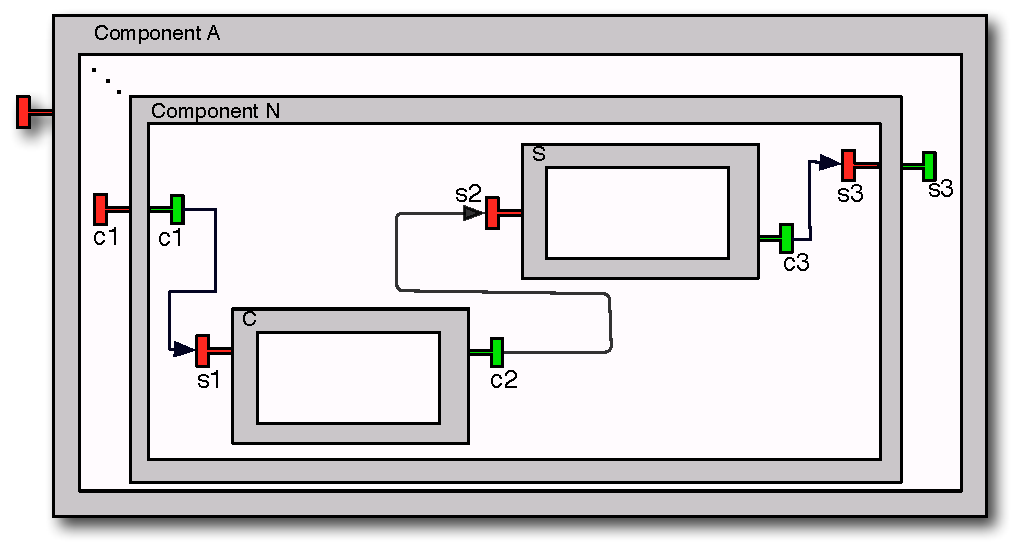
\includegraphics[scale=0.7]{figures/chapter4/bindings.pdf}
		\caption{\textsf{binding} examples}
		\label{fig:bindingsdemo}		
	\end{figure}		

	\noindent From left to right, the three bindings illustrated by Figure \ref{fig:bindingsdemo} are depicted by
	Listing \ref{lst:exbindings}.

	\lstinputlisting[language=Coq, stepnumber=1, 
	                        caption={\textsf{binding} examples in \textsc{Mefresa}}, 
	                        label=lst:exbindings]{listings/chapter4/bindings.tex}

	\noindent where \textbf{pb} is \textsf{(Ident "Component A" :: ... :: Ident "Component N" :: nil)}, i.e., the adequate 
	\textsf{path} for the bindings hold by the \textsf{component} named \textit{"Component N"}.


	%maybe i should some more prose and a complete component term ==> component term needed to justify language
	
\subsubsection{A complete example}
		
				
		Having discussed the three core elements of the \ac{GCM}, it still remains to see them all together at once.
	For the sake of clarity, in the following we show how the aforementioned
	\textsf{component} \textit{"Component N"} is represented in \textsc{Mefresa}. First, let us
	 mechanize its subcomponent \textit{"C"}. Listing \ref{lst:rex1} depicts such a task.
		
	\lstinputlisting[language=Coq, stepnumber=1, 
	                       caption={Model for \textsf{component} \textit{"Component N"} (part 1 of 3)}, 
	                       label=lst:rex1]{listings/chapter4/rex1of3.tex}
	
	
	\noindent Lines 1-4 define some parameters for this example. Parameter \textbf{p}
	stands for the \textsf{path} of \textsf{component} \textit{"Component N"}. Then,
	 \textsf{iclC}, \textsf{sigS1} and \textsf{sigC2} stand for the implemenetation class
	 of \textsf{component} \textit{"C"}, \textsf{signature} of \textsf{interface S1} and 
	 \textsf{signature} of \textsf{interface C2}, respectively. Line 6 defines
	 the \textsf{path} for \textsf{component} \textit{"C"} by appending the appropriate \textsf{identifier}.
	 The definition of \textsf{component} \textit{"C"} \textit{per se} starts at line 8. Its understanding
	 should pose no doubt. It is set with the default control level value \textsf{Configuration},
	 has no subcomponents --- thus represented by an empty list (line 11) --- 
	 features two interfaces adequately
	 defined in lines 13-16, and has no bindings (line 18).
	
	
	\lstinputlisting[language=Coq, stepnumber=1, 
	                      caption={Model for \textsf{component} \textit{"Component N"} (part 2 of 3)}, 
	                       firstnumber=19,
	                      label=lst:rex2]{listings/chapter4/rex2of3.tex}	
	
	
	\noindent	 Sub\textsf{component} \textit{"S"} has the same structure and 	
	is naturally defined analogously. Its mechanization is depicted by Listing \ref{lst:rex2}.
	Note that both \textsf{component}s \textit{"S"} and \textit{"C"} possess the same 
	\textsf{path} (line 23), we assign a new variable for the sake of clarity.
	 
	\lstinputlisting[language=Coq, stepnumber=1, 
	                      caption={Model for \textsf{component} \textit{"Component N"} (part 3 of 3)}, 
	                       firstnumber=36,
	                      label=lst:rex3]{listings/chapter4/rex3of3.tex}		
	
	\noindent For last, composite \textsf{component} \textit{"Component N"} is illustrated by
	Listing \ref{lst:rex3}. The careful reader may notice the definition of the variable \textsf{pN}
	(line 39). This, is subsequently used as \textsf{path} for \textsf{component} \textit{"Component N"}'s
	\textsf{interface}s and \textsf{binding}s. Indeed, all of its constituents (sub\textsf{component}s,
	\textsf{interface}s and \textsf{binding}s) possess the same \textsf{path}. 
	
		The remaining of its mechanization should pose no doubt. It mainly differs from
	the two precedent mechanizations (Listing \ref{lst:rex1} and Listing \ref{lst:rex2}) in
	that it also possesses sub\textsf{components}, \textsf{interface}s of \textsf{internal} visibility,
	and \textsf{binding}s.
	

\subsection{Well-formed component architectures}
\label{sub:wellformed}

	 The above definition of the \ac{GCM} core elements allowed us to see how to compose components.
	 Indeed, by exploiting their hierarchical structure one can build arbitrary complex
	 architectures. Yet, randomly constructing these by solely respecting the 
	 inherent typing rules for the \textsf{component}, \textsf{interface}
	 and \textsf{binding} structures, is naturally insufficient w.r.t.
	 the \ac{GCM} specification compliance. In order to be certain that we are
	 building valid \ac{GCM} architectures we need to formalize its requirements.
	
%%%%
	
		Let us define a predicate concerning the \textit{well-formedness} of a \textsf{component}.
	Listing \ref{lst:wfcomp} depicts such predicate. %, where the notation \textsf{(object-->field)} is used 
	%for projections: \textsf{(c-->subcomps)} stands for the subcomponents of \textsf{c}, etc.			
	
	
		\lstinputlisting[language=Coq, stepnumber=1, 
	                        caption={well-formed \textsf{component} definition}, 
	                        label=lst:wfcomp]{listings/chapter4/wfcomp.tex}

	\noindent Basically, a \textsf{component} is \textit{well-formed} if all its subcomponents
	are individually well-formed (line 3), and do not possess common identifiers (line 4). Further,
	its interfaces and bindings must also be well-formed (lines 5-6). 

	
	The intended meaning of the
	\textsf{unique\_ids} predicate should be clear from its name. 
	Listing \ref{lst:uniqueids} depicts its definition.
	
	\lstinputlisting[language=Coq, stepnumber=1, 
	                        caption={\textsf{unique\_ids} predicate definition}, 
	                        label=lst:uniqueids]{listings/chapter4/uniqueids.tex}

	\noindent It is composed by two constructors: \textsf{Unique\_Base} and \textsf{Unique\_Step}.
	The former simply states that an empty list has indeed unique identifiers. The latter covers
	the case when the parameter \textsf{l} is composed by a head element
	\textsf{c} and a tail list \textsf{r} (line 13). The subsequent two premisses
	ensure that \textsf{c}'s identifier is not equal to the \textsf{component}s' identifier 
	in the tail \textsf{r} (line 14), and for last, the predicate itself is applied to the tail
	\textsf{r} (line 15). Concerning the \textsf{not\_in\_l} predicate, it is essentially	
	defined in the same manner. The \textsl{NotInNil} constructor deals with the case
	when the parameter \textsf{l} is empty (lines 2-3). The \textsf{NotInStep} constructor deals with the
	more interesting case, when \textsf{l} is composed by a head element \textsf{c} 
	and a tail \textsf{r} (line 5).	\textsf{c}'s identifier is checked against
	parameter \textsf{i} (line 6), and the predicate itself is recursively applied
	to the tail \textsf{r} (line 7).
	
	
		Regarding \textsf{component}'s \textsf{interface}s, the sole requirement is that they are uniquely identifiable
	by their \textsf{id} and \textsf{visibility} values. Listing \ref{lst:unique} formalizes
	this constraint.			
	
	\lstinputlisting[language=Coq, stepnumber=1, 
	                        caption={\textsf{well\_formed\_interfaces} predicate definition}, 
	                        label=lst:unique]{listings/chapter4/unique.tex}
	
	\noindent Indeed, the \textsf{not\_in\_l\_pairs} predicate does the main work.
	The expression \textsf{not\_in\_l\_pairs i v l} should be read as: there is no
	\textsf{interface} in \textbf{l} that possesses both the same identifier and
	visibility values as \textbf{i} and \textbf{v}, respectively.	
	The constructor \textsf{NotInPairsNil} covers the case where \textbf{l}
	is empty --- it is simply true by definition (line 2). 
	The constructor \textsf{NotInPairStep} accounts for the case where \textbf{l}
	contains at least one element: a head element \textbf{int} 
	followed by a tail \textbf{r} (line 4). 	
	The arguments \textbf{i} and \textbf{v} are checked against the identifier and
	\textsf{visibility} values of \textbf{int} (line 5), and finally the same process is applied to
	the tail \textbf{r}, making the predicate recur (line 6).
	
		The understanding of the \textsf{unique\_pairs} predicate should pose no doubt, it
	essentially follows the same rationale, and relies on \textsf{not\_in\_l\_pairs} to achieve
	its intended significance.


		Before further proceeding into well-formedness concerns, let us define an auxiliary function
	concerning the indexation of \textsf{interface}s. Listing \ref{lst:itfindex} defines a function
	retrieving one \textsf{interface} from a list of \textsf{interface}s by its identifier and
	\textsf{visibility} values.

\lstinputlisting[language=Coq, stepnumber=1, 
	                        caption=Function to find an \textsf{interface} by its identifier and \textsf{visibility} values, 
	                        label=lst:itfindex]{listings/chapter4/itfindex.tex}

	\noindent Its comprehension is straightforward. The \textit{head} element \textsf{i}
	of parameter \textsf{l} is checked for its identifier and \textsf{visibility} values (line 5). 
	Should they be equal to parameters \textsf{id} and \textsf{v}, respectively, 
   \textsf{interface} \textsf{i} is returned (line 6). Otherwise,
   the function recurs in the \textit{tail} \textsf{r} (line 8). Naturally, no \textsf{interface} is returned if 
   \textsf{l} is empty (line 4). Moreover, a convenient notation is defined (line 11): \textsf{l[id, v]} stands
   for \textsf{get\_interface id v l}.
   
    

%%%binding wf
	The last remaining piece concerns the well-formedness of \textsf{binding}s. 
	Listing \ref{lst:wfbinding} illustrates its definition.

			\lstinputlisting[language=Coq, stepnumber=1, 
	                        caption={\textsf{well\_formed\_bindings} predicate definition}, 
	                        label=lst:wfbinding]{listings/chapter4/wfbinding.tex}
	
	\noindent The careful reader may notice one particularity regarding the definition of the
	\textsf{well\_formed\_bindings} predicate: unlike  \textsf{well\_formed\_component} and
	\textsf{well\_formed\_interfaces}, it takes more than one parameter into account.
	A binding is hold by a component and serves as a means for 
	components to communicate with each other, and thus cannot 
	exist by itself. As such, it should come as no surprise that its
	well-formedness depends on its surroundings, i.e. the
	components and interfaces involved in its definition.
			
	Regarding the	mechanization depicted by Listing \ref{lst:wfbinding}, its 
	understanding should pose no doubt.  Basically, the predicate \textsf{valid\_binding}
	is applied to all bindings $b \in lb$ (line 9). This, performs a case analysis
	on \textit{b} and its validity is checked depending on whether it is a 
	\textsf{normal}, \textsf{export} or \textsf{import binding} (lines 2-5).
	 For instance, Listing \ref{lst:nmbinding} depicts the \textsf{normal\_binding} predicate.
		
	\lstinputlisting[language=Coq, stepnumber=1, 
	                        caption={\textsf{normal\_binding} predicate definition}, 
	                        label=lst:nmbinding]{listings/chapter4/normalbinding.tex}
	
	\noindent  A \textsf{normal binding} establishes a binding between two sub\textsf{component}s, and	
	is composed by four identifiers denoting
	(1) the name of the \textsf{component} holding the \textsf{client interface}, (2) the name
	of this \textsf{client interface}, (3) the name of the \textsf{component} holding the \textsf{server interface}, and
	finally (4) the name of this \textsf{server interface}. Therefore, checking its validity boils down
	to ensuring that these identifiers refer to existing client and server interfaces.
	The parameters \textsf{idC1} and \textsf{idC2} contain the name of the \textsf{component}s
	involved in the \textsf{binding}. These are both supposed to be indexed in \textsf{lc} (line 3),
	if that is not the case it means that the binding is not valid and \textsf{False} is 
	returned (line 9). If both components \textsf{c1} and \textsf{c2} are found, then 
	\textsf{idI1} and \textsf{idI2} are supposed to be indexed in their list of \textsf{interface}s, respectively.
	Further, since it is a \textsf{normal binding}, it implies that it is established between 
	two \textsf{external} interfaces (line 5). Failure to find the referred \textsf{interface}s means that
	the binding is not valid and \textsf{False} is returned (line 7). Otherwise,
	its validity depends on whether 
	the \textsf{interface}s \textsf{i} and \textsf{i'} are indeed of \textsf{client} and \textsf{server} roles, respectively (line 6).
			
		As expected, the predicates \textsf{export\_binding} and \textsf{import\_binding} are defined
	analogously. The main difference lies in the fact that these \textsf{binding}s are not between two sub\textsf{component}s,
	but between a parent \textsf{componen}t and one sub\textsf{component} (or vice-versa). 
	

\subsubsection{A first well-formedness proof}
	
	%running example
	Having defined	 our well-formedness predicates it is time to see them in action. Let us retake our
	running example concerning \textsf{component} \textit{"Component N"} discussed in
	Subsection \ref{sub:core} (see Listing \ref{lst:rex1}, Listing \ref{lst:rex2} and Listing \ref{lst:rex3}). 
	
		First, let us reason about its sub\textsf{component}s well-formedness. Lemma \ref{th:wflemmaexC}
	addresses the well-formedness of \textsf{component} \textit{"C"}.
				
			
	\begin{lemma} \label{th:wflemmaexC} 
	\lstinputlisting[language=Coq, numbers=none]{listings/chapter4/wflemmaC.tex}				
	
		We start by applying the \textsf{WellFormedComponent} constructor, which yields
		four subgoals to discharge.			
		  The first and second subgoals concern its subcomponents: their 
		individual well-formedness and the uniqueness of their identifiers.		
		Since it has no	subcomponents both premisses are trivially established. 
			
			The third subgoal regards the well-formedness of its interfaces. These need
			to be uniquely identifiable by the tuple composed by their identifier and
			visibility values. It is clearly the case as it only possesses two external interfaces
			named \textsf{s1} and \textsf{c2}.			
			
			Finally, the fourth subgoal requires the well-formedness of its bindings. This is also
			trivially proved as it is a primitive component and thus has no bindings.
			And therefore the proof concludes. \qed
	\end{lemma}				

			
	\noindent As expected, proving the well-formedness of \textsf{component} \textit{"S"} follows
	the same rationale. Indeed, both	possess the same structure. Regarding 
	\textsf{component} \textit{"Component N"}, its well-formedness is tackled by Lemma \ref{th:wflemmaexN}. 
				
	\begin{lemma} \label{th:wflemmaexN} 
	\lstinputlisting[language=Coq, numbers=none]{listings/chapter4/wflemmaN.tex}				
	
		Applying \textsf{WellFormedComponent} yields four subgoals to prove.	
		
		It possesses two subcomponents (\textsf{component} \textit{"C"} 
		and \textsf{component} \textit{"S"}), both are well-formed as previously discussed.	Further,
		their identifiers are different, and therefore the first two subgoals are easily discharged.
		
			It features four interfaces. Two of external visibility, and two of internal visibility.
		Indeed,	 some share the same identifier, yet, these are of different visibility value, and thus still
		uniquely identifiable.
		
			For last, its three bindings are established from and to existent components/interfaces, and from
			client to server. Thus, also well-formed, and the proof concludes. 	\qed
	\end{lemma}	
	

%\subsubsection{General properties: well-formedness corollaries}	
	
	
\subsection{Well-typed component architectures}
\label{sub:welltyped}

	A \textsf{component} may be well-formed but still unable to start execution. Indeed, its
	 well-formedness guarantees involve important aspects regarding its composition, yet,
	 further insurances are needed for the overall good functioning of the system in terms of its 
	 application dependencies. These are dictated by simple typing rules (see \cite[p. 22]{ETSI2009:GCMADL}).	 
	 
		An \textsf{interface} possesses \textsf{cardinality} and \textsf{contingency} attributes. These determine
	its supported communication model and the guarantee of its functionality availability, respectively.
	For instance, as dictated by the \ac{GCM} specification, for proper system execution 
	we must ensure that \textsf{singleton} \textsf{client} \textsf{interface}s 
	are bound at most once. Indeed, for \textsf{client} \textsf{interface}s only those with \textsf{multicast} \textsf{cardinality}
	are allowed to be bound more than once. 
	
		Analogously, similar constrains apply to the \textsf{interface}s' \textsf{contingency} attribute. An \textsf{interface} 
	of \textsf{mandatory}	\textsf{contingency}  is guaranteed to be available at runtime. This is rather obvious for \textsf{server}
	\textsf{interface}s as they implement one or more service methods, i.e., they do have a functionality of their own. \textsf{Client}
	\textsf{interface}s however, are used by service methods that require other service methods to perform their task. It therefore follows
	that a \textsf{client} and \textsf{mandatory} \textsf{interface} must be bound to another \textsf{mandatory} \textsf{interface} of
	\textsf{server} \textsf{role}.  As expected, \textsf{interface}s of \textsf{optional} \textsf{contingency} are not guaranteed to be available.
			
	\textsc{Mefresa} captures these requirements by defining a well-typed predicate as depicted by Listing \ref{lst:wtyped}.


	\lstinputlisting[language=Coq, stepnumber=1, 
	                        caption={\textsf{well\_typed} predicate definition}, 
	                        label=lst:wtyped]{listings/chapter4/wtyped.tex}

	\noindent  Its definition is straightforward, it is a simple conjunction between two more interesting 
	predicates: \textsf{sound\_cardinality} and \textsf{sound\_contingency}. Listing \ref{lst:scont} depicts the latter.
	
		
	\lstinputlisting[language=Coq, stepnumber=1, 
	                        caption={\textsf{sound\_contingency} predicate definition}, 
	                        label=lst:scont]{listings/chapter4/scont.tex}
	
  \noindent As shown by the \textsf{sound\_contigency} predicate we split its definition
		into \textsf{subc\_client\_external\_mandatory\_itfs\_are\_bound} 
       and \textsf{client\_internal\_mandatory\_itfs\_are\_bound}. Indeed,	the former checks the \textsf{external}
       \textsf{interfaces}, while the latter the \textsf{internal} ones. 
           
       
	       \lstinputlisting[language=Coq, stepnumber=1, 
	                        caption={\textsf{client\_internal\_mandatory\_itfs\_are\_bound} predicate definition}, 
	                        label=lst:cimi]{listings/chapter4/cimi.tex}
       
      Listing \ref{lst:cimi} depicts the \textsf{client\_internal\_mandatory\_itfs\_are\_bound} predicate.      
      Basically, we need to check that for all \textsf{client}, \textsf{internal}, and
       \textsf{mandatory} \textsf{interfaces} of some \textsf{component} \textbf{c} (lines 3-4), 
       their \textsf{interface} recipients list originating from \textsf{export bindings} 
       are non-empty --- i.e. at least bound once --- (lines 5-7) and of \textsf{mandatory} \textsf{contingency} (line 8). 	
	   Naturally, the same applies recursively to the remaining of the \textsf{component} hierarchy (lines 9-10).	
	
		  As expected, the \textsf{subc\_client\_external\_mandatory\_itfs\_are\_bound}  predicate is defined analogously
	  w.r.t. the sub\textsf{component}s \textsf{external} \textsf{interface}s. For the sake of completeness,
	  Listing \ref{lst:cemi} depicts its definition.
	  
	   \lstinputlisting[language=Coq, stepnumber=1, 
	                        caption={\textsf{subc\_client\_external\_mandatory\_itfs\_are\_bound} predicate definition}, 
	                        label=lst:cemi]{listings/chapter4/cemi.tex}
	
	%%%should i add text here?
		
%%%%%%	
\subsubsection{A first well-typedness proof}
	
	Retuning to our running example from Subsection \ref{sub:core}, let us discuss
	\textsf{component} \textit{"Component N"}'s well-typedness.
	
	 First, we need to establish that \textsf{component} \textit{"Component N"} has indeed
	 a sound \textsf{contingency}. Lemma \ref{th:scontlemma} addresses this concern.
	 	 
		
\begin{lemma} \label{th:scontlemma} 
	\lstinputlisting[language=Coq, numbers=none]{listings/chapter4/scontlemma.tex}		
	
	By unfolding the statement to prove, we can see that it is actually a 
	conjunction of two predicates: subc\_client\_external\_mandatory\_itfs\_are\_bound 
	and client\_internal\_mandatory\_itfs\_are\_bound. 
	
		 For the former we start by applying its constructor \textsf{CEMI\_Bound} and
	get two subgoals to discharge. The first one requires that all subcomponents'
	client, external and mandatory interfaces are indeed bound, 
	while the second one recursively requires the same for the component hierarchy 
	inner levels. 
		Component "Component N" contains two subcomponents: "C" and "S". Both
	possess one client interface, "c2" and "c3", respectively. Yet, only "c2" is of mandatory 
	contingency, and it is indeed adequately bound through a normal binding
	to "s2" (which is also of mandatory contingency). Proving the second subgoal 
	is straightforward: both subcomponents "C" and "S" are primitive, thus possess no 
	subcomponents. And therefore subc\_client\_external\_mandatory\_itfs\_are\_bound 
	is discharged.
	
		Proving client\_internal\_mandatory\_itfs\_are\_bound follows the same rationale.
	Only the interface "c1" from component "Component N" is concerned and it is indeed
	adequately bound to "s1". \qed
\end{lemma}

	\noindent The demonstration that \textsf{component} \textit{"Component N"}
	has a sound cardinality follows the same spirit. Basically, 	we need to exhaustively
	check that all concerned \textsf{interface}s are meeting the cardinality-related 
	requirements. For such simple \textsf{component} architecture, it is easy to see
	that it is indeed the case as all the present \textsf{interface}s are of \textsf{singleton}
	\textsf{cardinality} and are all bound at most once. 
	
		Finally, we can show that \textsf{component} \textit{"Component N"} is 
	indeed well-typed. This is illustrated by Lemma \ref{th:wtlemma}.
		

\begin{lemma} \label{th:wtlemma} 
	\lstinputlisting[language=Coq, numbers=none]{listings/chapter4/wtlemma.tex}		
		Establishing the well-typedness of component "Component N" boils down to
	proving that it has a sound contingency and a sound cardinality. This is clearly the case
	as previously discussed. \qed
\end{lemma}

	%%should i put text here..

%%%%
\subsection{Well-formedness and well-typedness decidability}
\label{sub:wfdec}


	A \textsf{component} that is both well-formed and well-typed is said to be ready to 
	start execution. The definition of these predicates gives us the ability to interactively prove inside Coq	
	that a \textsf{component} system can, or not, start its execution. The burden of such a demonstration for one  
	component \textsf{c} will therefore inherently depend on the complexity of \textbf{c}. In fact, one may wonder
	about the feasibility of undertaking such proof, i.e., whether it is indeed possible to actually prove
	or disprove that \textbf{c} is well formed and well typed\footnote{It should be noted that
	we are in the context of Coq's constructive logic, theorems that are true in 
	classical logic (i.e. the excluded middle) may not be provable in Coq.}.	 In other words, it is
	worth knowing that both predicates are \textit{decidable}.
	
		First, we need a predicate expressing decidability. Listing \ref{lst:dec} depicts one such
	predicate.		
	
	   \lstinputlisting[language=Coq,  
	                        caption=\textsf{decidable} predicate definition, 
	                        label=lst:dec]{listings/chapter4/dec.tex}
	
	\noindent Its definition is rather simple: it takes one proposition and returns the disjunction of this 
	proposition itself with its negation. For our purposes, we shall use it for our
	well-formedness and well-typedness predicates. Indeed, proving them decidable is of 
	paramount importance, it ensures the existence of an algorithm capable of automatically 
	determining their valuation.

	Generally, there are two approaches for proving a predicate's decidability. On the one hand,
	one can attempt to prove it by exploiting the structure of the involved parameters, showing that for all
	of its constructors it is indeed possible to infer a \textit{True} or \textit{False} valuation. 
	On the other hand, one can	write a function that acts as its computational counterpart, i.e.,
	it returns a boolean value, \textit{true} or \textit{false}, in accordance with the predicate's 
	valuation. Then, one needs to show that this function is \textit{sound} --- whenever it returns 
	\textit{true} the predicate's valuation is \textit{True} ---, and \textit{complete} --- whenever
	 the predicate's valuation is \textit{True}, the function returns \textit{true}. Such 
	 functions are often called \textit{decision procedures}. Finally, proving the predicate's decidability
	 has now become trivial since it is intrinsically related with this boolean function.
	
		In the following, we use the first approach for demonstrating the decidability of the
	\textsf{well\_formed\_component} predicate, and the second approach for tackling the decidability 
	of the \textsf{well\_typed} predicate. 
		
	

\subsubsection{Well-formedness decidability}
	
				
		As shown by Listing \ref{lst:wfcomp}, the \textsf{well\_formed\_component} predicate is
	composed by other predicates: \textsf{unique\_ids}, \textsf{well\_formed\_interfaces}, and
	\textsf{well\_formed\_bindings}. Naturally, proving their decidability is required in order
	to demonstrate that  \textsf{well\_formed\_component} is decidable.	
	
		For instance, let us consider the \textsf{unique\_ids} predicate. As shown by Listing
		\ref{lst:uniqueids}, its definition includes the \textsf{not\_in\_l} predicate (see Listing \ref{lst:uniqueids}). As such,
		the first step is to prove its decidability. This is demonstrated by Lemma \ref{th:notindec}. 
				
		\begin{lemma} \label{th:notindec} 
		\lstinputlisting[language=Coq, numbers=none]{listings/chapter4/notindec.tex}		
		
			We start by applying induction on the structure of \textsf{l}, and thus
		obtain two subgoals. Both require the original goal but applied 		
		to an empty list, and to a list composed by a head element \textsf{c}
		and a tail \textsf{l}.
		
			The first subgoal is trivial. We recall that the \textsf{decidable} predicate 
		actually stands for a disjunction. In particular, for this 
		case: \textsf{not\_in\_l id nil $\lor$ $\neg$not\_in\_l id nil}. Its left-hand side
		proposition its evidently true. Proving \textsf{not\_in\_l id nil} can easily be achieved by applying
		the \textsf{NotInNil} constructor, at which point we only need to show that
		\textsf{nil = nil}, which is discharged by reflexivity. 
		
			The second subgoal requires the demonstration of \textsf{decidable (not\_in\_l id (c::l))} by assuming
		\textsf{decidable (not\_in\_l id l)} as induction hypothesis. At this point we can safely assume that
		\textsf{(c ->id) = id} is either true or false. 
		
		For the first case, we can show that the right-hand side
		of our goal is true. Indeed, since \textsf{(c ->id)} is equal to \textsf{id}, then it is easy to see that
		\textsf{not\_in\_l id (c::l)} is false. Thus, we need to prove the negation of false, which is a		
		tautology. 
		
		For the second case, we need to use the induction hypothesis. We  know that 
		\textsf{(not\_in\_l id l)} is either true or false. If it this true, then we can show that
		\textsf{not\_in\_l id (c::l)} is also true. Indeed, since \textsf{(c ->id) = id} is false
		we have all the ingredients to discharge this subgoal by applying the \textsf{NotInStep} 
		constructor. If it is false, then it follows that \textsf{not\_in\_l id (c::l)} is also false, as we
		have in context the negation of one of its premises. And thus the proof concludes. \qed		
		\end{lemma}
				
		Having demonstrated \textsf{not\_in\_l}'s decidability, we are now in a position to
	address the \textsf{unique\_ids} predicate. Its decidability is discussed
	by Lemma \ref{th:uniquedec}.	
	
	\begin{lemma} \label{th:uniquedec} 
		\lstinputlisting[language=Coq, numbers=none]{listings/chapter4/uniquedec.tex}		
		
				We start by applying induction on the structure of \textsf{lc}. This, naturally yields
			two subgoals: we now need to demonstrate the original goal for an empty list,
			and then for a list composed by a head element \textsf{c} and a tail list \textsf{l}.
			
				The first subgoal is trivial, we can easily demonstrate \textsf{unique\_ids nil}
			by applying its \textsf{Unique\_Base} constructor.				
				
				The second subgoal is more elaborated. From the induction hypothesis
			we know that \textsf{unique\_ids lc} is either true or false. Further, 
			from Lemma \ref{th:notindec} we know that this is also the case for 
			\textsf{not\_in\_l (c ->id) lc}. We need to consider all their pairwise 
			combinations, and thus we have four cases to deal with. 
			
				For the first case, we have both assumptions with a valuation of true. 
				It this therefore easy to show that \textsf{unique\_ids (c :: lc)} holds by applying
			the \textsf{Unique\_Step} constructor.
			
				The remaining three cases possess at least one assumption with
			a valuation of false. Thus, it is always possible to show that
			\textsf{$\neg$ unique\_ids (c :: lc)} holds, as we always have
			the negation of one of its premises in context. And thus we can conclude
			the proof. \qed
	\end{lemma}
	
		\noindent Proving the decidability of the \textsf{well\_formed\_interfaces} and
	\textsf{well\_formed\_bindings} predicates follow the same rationale. We account for
	all possible cases by recurring to structural induction, and reasoning symbolically on
	the parameters. However, it should be noted that \textsf{well\_formed\_component c} 
	also possesses a premise involving a nested recursive call: \textsf{$\forall c',\ c' \in (c.subcomps)
	\rightarrow well\_formed\_component \ c'$}. Alas, coping with 
	such definitions in Coq is somewhat cumbersome, and requires delving into its
	intricacies. In the following, we demonstrate an approach that can be seen as a general
	recipe for dealing with such cases.
	
			First, let us prove an auxiliary lemma that is somewhat peculiar: it is possible to decide that
	all components in an empty list are well-formed. Lemma \ref{th:wflnil} demonstrates this.			
			
		\begin{lemma} \label{th:wflnil} 
		\lstinputlisting[language=Coq, numbers=none]{listings/chapter4/wflnil.tex}
		
		We can easily show the left-hand side of our goal: 
		$\forall c,\ c \in nil \rightarrow$ well\_formed\_component\ c. This means that
		we have $c \in nil$ as an assumption, which is always false.				
		Since from false anything follows, we can conclude the proof. \qed
	\end{lemma}				


	\noindent Having dealt with the case where the list of \textsf{component}s is empty,
	let us now cope with  the case where it is composed by a head element and a tail.
	For this case however, as demonstrated by Lemma \ref{th:wfcons}, we shall use
	some parameters to establish the proof. Basically, the parameters include the
	decidability of the well-formedness of a \textsf{component} \textbf{c}, and the 
	decidability of the well-formedness of all \textsf{component}s in a list \textbf{lc}.
	Then, we want to show that all \textsf{component}s in (\textsf{cons} \textbf{e} \textbf{lc})
	are also well-formed. 

		\begin{lemma} \label{th:wfcons} 
		\lstinputlisting[language=Coq, numbers=none]{listings/chapter4/wfcons.tex}		
			
			From the \textsf{Hc} hypothesis we know that well\_formed\_component \textbf{c}
			is either true or false. If it is false, then it evidently follows that $\neg (\forall e,\
			e \in (cons\ c\ lc) \rightarrow$ well\_formed\_component e). We only need to
			instantiate \textbf{e} with \textbf{c} to see that it is the case. If it is true however,
			we need to account for two other possibilities: from \textsf{Hlc} we know that ($\forall$ e, 
			e $\in$ lc $\rightarrow$ well\_formed\_component e) is either true or false.
			If it is true, then we have all the necessary assumptions to prove that
			the left-hand side of our goal holds:
			if \textbf{e} is instantiated with \textbf{c}, then we can show it with
			\textsf{Hc}, otherwise if $\textbf{e} \in \textsf{lc}$, then we can show it
			with \textsf{Hlc}. If it is false however, then we can show the right-hand side
			of our goal by analogous reasoning. \qed
	\end{lemma}	
	
		 The last remaining ingredient before proceeding to the main proof is
	depicted by Lemma \ref{th:wfclc}. Basically, we prove the decidability of the well-formedness of 
	all \textsf{component}s member of a list, while having as parameter the 
	decidability of the well-formedness of all \textsf{component}s. Indeed, 
	it seems a rather strange lemma to prove. However, it is of paramount 
	importance for the applicability of this approach. 
	We exhibit its proof with the associated Coq script in order
	to further emphasize the peculiarity of the approach. 
					
	\begin{lemma} \label{th:wfclc} \textit{well_formed_component_lc_dec:}
		\vspace{-0.2cm}
		\lstinputlisting[language=Coqfix, numbers=left, numberfirstline=false, stepnumber=1, firstnumber=2]{listings/chapter4/wfclc.tex} 
		
		%\vspace{-0.8cm} \qed
	\end{lemma}	
	
	\noindent  The first thing to note is the use of the \textsf{fix} construct (line 5). This allows
	to define anonymous recursive functions. Basically, the proof is achieved by defining
	a recursive function that pattern matches on its parameter \textsf{lc} and uses Lemma \ref{th:wflnil}
	and Lemma \ref{th:wfcons} to adequately cover all the cases (lines 8-10). For last, the careful reader may 
	wonder about the use of \textit{Defined} instead of \textit{Qed} (line 12). 
	This makes Coq keep the proof of Lemma \ref{th:wfclc} --- it exposes its 
	recursive nature to a caller --- while with \textit{Qed} it would become 
	\textit{opaque}. 
		
		Finally, we are in a position to prove the decidability of the \textsf{well\_formed\_component}	
	predicate for all \textsf{component}s \textbf{c} as demonstrated by Theorem \ref{th:wfdec}. 
	We also exhibit its proof as a Coq script 
	to illustrate how the approach described so far is put into practice.	
	
	\begin{theorem} \label{th:wfdec} \textit{well_formed_component_dec:}
	\vspace{-0.2cm}
		\lstinputlisting[language=Coq, numbers=left, firstnumber=2]{listings/chapter4/wfdec.tex}	
		%\vspace{-0.9cm} \qed
	\end{theorem}

	\noindent We start the proof by performing structural induction on the first argument through
	the \textsf{fix} tactic\footnote{Not to be confused with the previously mentioned 
	\textsf{fix} construct for recursive functions.} and introduce in the 
	context \textsf{component} \textbf{c}'s constituents (identifier, path, implementation class, ...) (line 4). 
	The \textsf{fix} tactic also introduces a new hypothesis in the context, 
	named as the current theorem, and with the same type as the goal. Indeed, this is an odd
	behaviour, and one may be tempted to use this new hypothesis to discharge the goal, but that would make
	Coq reject the proof. In short, proofs done with \textsf{fix} are required to satisfy a syntactic 
	\textit{guardedness} criterion, and attempting to directly discharge a goal with the hypothesis it
	introduces violates this criterion.	
	
		We introduce the proof that all sub\textsf{component}s of \textbf{c} are
	well-formed into our context and name it \textsf{IHp\_dec} (lines 5-6). Further, we
	remove the hypothesis introduced by \textsf{fix} since we will not use it anymore (line 7).
	Then, we use the \textsf{Guarded} command to check that Coq's guardedness 
	condition is satisfied (line 8). It is not a tactic, it does not affect the state of the
	proof. Its sole purpose is to inform about the compliance of this guardedness condition
	at the current state of the proof, rather than having to wait until its conclusion.

		At this point, the main work for this proof is done. The remaining simply
	accounts for all possible cases regarding the well-formedness decidability of 
	the involved predicates (lines 10-12), and discharges them adequately (lines 16-17).
	

		Finally the decidability of our \textsf{well\_formed\_component} is proved. Undeniably, 
	the burden of this approach is considerable. This is mainly due to the way Coq is able to cope
	with nested definitions such as the \textsf{component} datatype. Moreover, the behaviour 
	of the \textsf{fix} tactic is rather undocumented, and is generally not recommended. In fact, even in
	\textit{Cocorico}\footnote{Cocorico is the official Coq wiki, also known as \textit{The nonterminating Coq wiki}: \url{http://coq.inria.fr/cocorico/Home}} it is stated that \textit{"it is not advisable to use it (unless you know what you do)"}.
	Alas, there are situations where it is indeed required. Nevertheless, for more details on its intricacies the reader is pointed to 
	Gim\'enez's tutorial on recursive types \cite{Giménez98atutorial} for a very brief discussion on its use. 
	
	
	
\subsubsection{Well-typedness decidability}


	Having demonstrated the \textsf{well\_formed\_component} predicate decidable, it is time to cope
	with the \textsf{well\_typed} predicate. As mentioned earlier, we shall use a different approach
	to tackle this task: we define some functional code that act as the computational counterpart of the \textsf{well\_typed}
	predicate.
		
			Basically, we need a function that returns the boolean value \textit{true} whenever
		a \textsf{component} is well-typed, and the boolean value \textit{false} otherwise. Further, it must be able
		to do it for all \textsf{component}s given as input. Listing \ref{lst:wtbool} depicts such function.

		
	\lstinputlisting[language=Coq,  
	                        caption=\textsf{well\_typed\_bool} function definition, 
	                        label=lst:wtbool]{listings/chapter4/wtbool.tex}		
	
			
	\noindent Basically, it follows the same spirit as the \textsf{well\_typed} predicate (see Listing \ref{lst:wtyped}),
	except that it is composed by boolean functions rather than predicates. With no surprise, the definition
	of the \textsf{sound\_contingency\_bool} function also follows the same spirit as the \textsf{sound\_contingency}
	predicate (see Listing \ref{lst:scont}). Listing \ref{lst:soundcontbool} depicts its definition.	
	
		\lstinputlisting[language=Coq,  
	                        caption=\textsf{sound\_contingency\_bool} function definition, 
	                        label=lst:soundcontbool]{listings/chapter4/soundcontbool.tex}
	
	
	\noindent Indeed, the actual work is carried by the two boolean functions
	\textsf{client\_internal\_mandatory\_itfs\_are\_bound\_bool} and 
	\textsf{subcomponents\_client\_external\_mandatory\_itfs\_are\_bound\_bool}
	--- the computational counterparts of the predicates depicted in Listing \ref{lst:cimi} 
	and Listing \ref{lst:cemi}, respectively. Listing \ref{lst:cimitfs} depicts the former.		


	\lstinputlisting[language=Coqfix,  
	                        caption=\textsf{client\_internal\_mandatory\_itfs\_are\_bound\_bool} function definition, 
	                        label=lst:cimitfs]{listings/chapter4/cltintmandbool.tex}


   \noindent %Indeed, the definition of this nested recursive function is all but natural.
   %This is related with Coq's termination checker. We need to write it in this way so that Coq can automatically
   %infer that it terminates. 
 % Nevertheless, 
   Its understanding should pose no doubt. Basically, it uses an auxiliary function
   \textsf{client\_internal\_mandatory\_itfs\_are\_bound\_bool\_one} to check the \textsf{interface}s at the current 
   hierarchical level (line 4) and then recurs on the inner levels, i.e., on the 
   sub\textsf{component}s (lines 5-10).
   
	The function responsible for checking each hierarchical level individually is also fairly simple. Listing
	\ref{lst:cimitfsaux} illustrates its definition.

	\lstinputlisting[language=Coqfix,  
	                        caption=\textsf{client\_internal\_mandatory\_itfs\_are\_bound\_bool\_one} function definition, 
	                        label=lst:cimitfsaux]{listings/chapter4/cltintmandboolaux.tex}


	\noindent  The parameter \textsf{li} holds a list of \textsf{interface}s. From these, it recovers those
	that are \textsf{client}, \textsf{internal}, and \textsf{mandatory} (line 3). If there are none meeting
	this criteria,  it simply returns \textit{true} (line 4): it means that there are no \textsf{interface}s that need
	to be checked. Otherwise, there is the need to check if the recipients of the \textsf{binding}s of these \textsf{interface}s are indeed
	of \textsf{mandatory} contingency (line 5). This is achieved by yet another auxiliary function depicted by
	Listing \ref{lst:cimitfsaux2}.
	
	\lstinputlisting[language=Coq,  
	                        caption=\textsf{check\_if\_recipients\_are\_mandatory\_aux} function definition, 
	                        label=lst:cimitfsaux2]{listings/chapter4/cltintmandboolaux2.tex}

	\noindent In short, it recurs through all \textsf{interface}s in parameter \textsf{li}, recovering
	their list of recipient \textsf{interface}s involved in \textsf{export} \textsf{binding}s (line 5). 
	These, must be non-empty and of \textsf{mandatory} \textsf{contingency} (lines 6-7) ---
	this is the purpose of the \textsf{not\_nil} and \textsf{check\_if\_mandatory} functions, respectively.
	Should that
	not be the case, the function returns \textit{false} (lines 8-9). Reaching an empty list makes the function
	return \textit{true} (line 4).
				
	
	Defining a function that checks if the \textsf{client}, \textsf{internal}, and \textsf{mandatory}
	\textsf{interface}s are adequately bound is not enough. We need to prove it correct, i.e., that it is
	indeed a reliable computational counterpart of the \textsf{client\_internal\_mandatory\_itfs\_are\_bound} 
	predicate. This is the purpose of Lemma	\ref{th:cltintmandcorrect}. In order to deal with its nested recursive
	nature we employ the same approach as seen for the decidability of the \textsf{well\_formed\_component} predicate.
	We omit the related auxiliary lemmas	and go straight to the main proof.		
	
	\begin{lemma} \label{th:cltintmandcorrect} 
	\lstinputlisting[language=Coq, numbers=none]{listings/chapter4/cltintmandcorrect.tex}		
		
		We start by applying the \textsf{fix} tactic and proceed by asserting the equivalence
	that we are trying to prove on the sub\textsf{component}s. We do this in an analogous
	manner as discussed for the \textsf{well\_formed\_component\_dec} theorem (see Listing \ref{th:wfdec}).
				
		We want to prove a logical equivalence and therefore the proof is divided in two parts. 
	The first part argues the soundness of the 
	\textsf{client_internal_mandatory_interfaces_are_bound_bool} function, i.e., 
	whenever it returns the boolean value true, the predicate \textsf{client_internal_mandatory_interfaces_are_bound}
	has indeed a valuation of True. The second part concerns its completeness: it is always able
	to return the boolean value true, provided that the predicate has a valuation of True.
	
		For the first part, we start by applying the \textsf{CIMI_Bound}	 constructor, thus obtaining two subgoals.
	For the first one, we need to establish that the concerned \textsf{interface}s are indeed bound to recipients
	of \textsf{mandatory} \textsf{contingency}. Since we have as hypothesis 
	\textsf{client_internal_mandatory_interfaces_are_bound_bool li lc lb = true}, it follows that
	\textsf{client_internal_mandatory_interfaces_are_bound_bool_one li lc lb = true} holds.
	By induction on \textsf{li}, and since we pattern match on the expression \textsf{li[Client, Internal, Mandatory]},
	we can generalize and consider two cases: either it yields an empty list,
	or not. If it is an empty list, then we have a contradiction, since
	the \textsf{CIMI_Bound} constructor introduced a \textsf{client}, \textsf{internal} and \textsf{mandatory}
	\textsf{interface} variable \textsf{$int \in li$} in our context. Thus we can discharge this subgoal.
	if it is not an empty list,	then we know that either \textsf{int} is the head of the list, or it is
	in the tail.  It it is the head of the list,  then we know that \textsf{not_nil lir \&\& check_if_mandatory lir}
	is true --- where \textsf{lir} is the list of recipients from \textsf{int}: \textsf{export_recipients (int->id) lb lc}.    
	Thus, we have in context all the necessary assumptions to prove our subgoal.	If it is in the tail of the list however,
	then we use the induction hypothesis, and can conclude this subgoal by unfolding and reducing the 
	adequate definitions.
	
	  For the second subgoal, we need to cope with the nested recursion on the sub\textsf{component}s. That is,
	we need to show that \textsf{client_internal_mandatory_interfaces_are_bound c'} holds, for $c' \in c.subcomps$.	
	From the beginning of this proof, we already asserted the equivalence for the sub\textsf{component}s. Thus, we can apply this 
	hypothesis and now need to show that \textsf{client_internal_mandatory_interfaces_are_bound_bool c' = true}, while having as 
	an assumption that \textsf{client_internal_mandatory_interfaces_are_bound_bool c = true}. Since we know it holds for the
	parent \textsf{component} \textbf{c}, then it must also hold for the sub\textsf{component} \textbf{c'} since the function definition
	recurs on all the \textsf{component} hierarchy. And thus we can conclude this subgoal. 
			
	The second part of this proof regards	the other implication: we now assume
	\textsf{client_internal_mandatory_interfaces_are_bound c} and try to prove
	\textsf{client_internal_mandatory_interfaces_are_bound_bool c = true}.
	It should be noted that the function in our goal is defined by a boolean conjunction
	between \textsf{client_internal_mandatory_interfaces_are_bound_bool_one li lc lb} and
	the recursive call on the sub\textsf{component}s.	Thus, we need to prove that both functions return
	the boolean value true. For the first one, we start by applying induction on \textsf{li}, yielding two subgoals.
	The first subgoal is trivial: if \textsf{li} is empty, so is \textsf{li[Client, Internal, Mandatory]}. Thus, the function
	returns the boolean value true, and we are left to show that \textsf{true = true}, which is trivially proved by reflexivity.
	For the second subgoal we need to show that 
	\textsf{client_internal_mandatory_itfs_are_bound_bool_one (a :: li) lc lb = true} holds. From the induction hypothesis
	we can conclude that \textsf{client_internal_mandatory_itfs_are_bound_bool_one li lc lb = true} holds,
	we now need to take care of the \textsf{interface} \textbf{a}. We need to consider three cases.
	If \textbf{a} is not of \textsf{client},
	\textsf{internal} and \textsf{mandatory} nature then it is irrelevant for the sake of this proof, and we can
	proceed to the subsequent case. If it is indeed of such nature, then it may or may not possess bounded recipients
	of \textsf{mandatory} \textsf{contingency}. If it is the case, then we can show our goal by computation, i.e.,
	we can reduce the term and eventually we get a \textsf{true = true} goal that is proved by reflexivity.
	If it is not the case, then we have a contradiction in our context w.r.t. 
	\textsf{client_internal_mandatory_interfaces_are_bound c} premisses.
	
	
		For the last part of this proof we need to show that the recursive call made on the sub\textsf{component}s
	indeed returns the boolean value true. We start by applying induction on \textsf{lc},  which yields two subgoals.
	The first subgoal is where there is no sub\textsf{component}: in this case the function simply returns true 
	and we can prove our goal by reflexivity. For the second subgoal we know there is at least one sub\textsf{component}
	and we can use the equivalence on the sub\textsf{component}s and the induction hypothesis to establish our goal.
	And thus the proof finally concludes. \qed	
	\end{lemma}	
	
	\noindent With no doubt, the above proof is long and laborious. Yet, it only tackles one of the involved
	functions. Indeed, analogous proofs are carried for the functions 
	\textsf{subcomponents\_client\_external\_mandatory\_itfs\_are\_bound\_bool} and 
	\textsf{sound\_cardinality\_bool}. We omit these proofs as they follow the same rationale. 
	
	Having established the equivalences between the relevant predicates and functions, we can 
	demonstrate Theorem \ref{th:wtcorrect}. We illustrate this proof with a Coq script 
	in order to emphasize how the approach is put into practice.

	\begin{theorem} \label{th:wtcorrect} \textit{well_typed_correctness:}
	\vspace{-0.2cm}
	\lstinputlisting[language=Coq, numbers=left, firstnumber=2]{listings/chapter4/wtcorrect.tex}		
	\end{theorem}


	\noindent Indeed, proving Theorem \ref{th:wtcorrect} is mostly achieved by using previous lemmas.
	And finally, Theorem \ref{th:wtdec} shows the decidability of the \textsf{well\_typed} predicate.
	We also demonstrate this proof as a Coq script as it further emphasizes how this general approach
	differs from the one employed for Theorem \ref{th:wfdec}.

	\begin{theorem} \label{th:wtdec} \textit{well_typed_dec:}
	\vspace{-0.2cm}
	\lstinputlisting[language=Coq, numbers=left, firstnumber=2]{listings/chapter4/wtdec.tex}		
	\end{theorem}


		Finally the decidability of the \textsf{well\_typed} predicate is demonstrated. Further, we also 
	defined a sound and complete decision procedure for the well-typedness valuation. Defining the 
	computational counterparts of the well-typedness specification was indeed	an elaborated task.	
	To this end, recent work \cite{CoqSpecCode:2012} aims at making such transformations automatic by
	extracting functional code from induction specifications and producing its proof of soundness.
	Yet, at the current stage of development it only works for a certain class of inductive 
	specifications, and a completeness proof seems out of reach.


		In this Section we discussed the mechanization of the \ac{GCM}. In particular, we discussed how 
	we used inductive definitions to model its core elements, and predicates to formally
	specify structure and typing requirements. Further, decidability of these predicates was also
	covered, ensuring that we can always determine whether a given component is compliant
	w.r.t. the \ac{GCM} specification. The remaining of this Chapter builds on top of these definitions 
	to develop a convenient language for manipulating  \ac{GCM} architectures, and to show
	pertinent examples.	
	

%% @@@@@@@@@@@@ Manipulating architectures with a simple \textsc{Operation} language
\section{An \textsc{operation} language for composing architectures}
\label{sec:op}


	%manipulating Coq term for component not really convenient... better to have dedicated language for that

		In the previous section, we saw how to use the \textsf{component} datatype to model a component hierarchy.
	 Yet, for more complex architectures, directly manipulating the  \textsf{component} datatype is not very convenient.
	 This is even more evident if we consider reconfigurations: the software architecture evolves 
	 and one needs a simple and elegant solution for coping with such structural changes. Moreover,
	 as mentioned in \cite{BHN:ICAS09} composing an architecture in a arbitrary manner can lead to an 
	 ”uncontrolled” architectural modification. Ensuring the consistency of the application's structure, both at 
	 deployment time and after performing a reconfiguration is thus of paramount importance.
	 
	  To this end, we define an \textsc{operation} language for manipulating \ac{GCM} architectures.
	In the following, we dedicate the remaining of this section delving intro its intricacies.
	 

\subsection{Syntax and semantics}
\label{sub:opsem}

		
	Before proceeding to the definition of our \textsc{operation} language \textit{per se}, let us introduce
	the notion of \textit{state}.	In most programming language definitions, a state is a structure
	that holds all the relevant information for a given program point, namely the mapping between
	the variables and their values. In our case, a \textsf{state} has the same shape as a \textsf{component}.
	Listing \ref{lst:state} depicts the \textsf{state} datatype.
	

	\lstinputlisting[language=Coq, label=lst:state, caption=\textsf{state} datatype, numbers=left]{listings/chapter4/state.tex}		


	\noindent The choice of the \textsf{component} structure to represent a \textsf{state} should come as no surprise.
	It holds all the relevant information w.r.t. the structure of a \ac{GCM} application, and has the advantage of
	being "well-known".
	
	 As further demonstrated by Listing \ref{lst:state}, and with no surprise, 
	 an empty \textsf{state} is a \textsf{component} that is located at 
	the \textit{root} of the hierarchy --- and thus with a \textsf{nil path} ---, and without any 
	 sub\textsf{component}s, \textsf{interface}s and \textsf{binding}s (lines 2-4). 
	
	Manipulating  the \textsf{state} structure is achieved with our aforementioned 
	\textsc{operation} language. Its syntactic categories for building 
	\ac{GCM} architectures are defined by Listing \ref{lst:operation}.
	
%	\begin{center}
%		\begin{tabular}{ l c c l }
% 		   operation   & ::=   &       &  \textbf{mk\_component} component\\
%			      &        &   \textbar\ & \textbf{mk\_interface} interface \\  
%			      &        &  \textbar\  & \textbf{mk\_binding} binding\\
%			      &        &   \textbar\ & \textbf{rm\_component} path id \\  
%			      &        &   \textbar\ & \textbf{rm\_binding}  binding\\  
%			      &        &  \textbar\  & operation; operation \\
%		          &        &  \textbar\  & \textbf{done} \\   
%	\end{tabular}
%	\end{center}
	
	\lstinputlisting[language=Coq, label=lst:operation, caption=\textsf{operation} datatype, numbers=left]{listings/chapter4/operation.tex}	

	
	\noindent The intended meaning of each constructor should raise no doubt. Basically, 
	our \textsc{operation} language allows us to make and remove components, make interfaces, and make and remove 
	bindings. Further, we can naturally compose \textsf{operation}s as a sequence. For this, we define a convenient
	notation as depicted by Listing \ref{lst:seq}.
	
	\lstinputlisting[language=Coq, label=lst:seq, caption=Notation for sequence of \textsf{operation}s, numbers=left]{listings/chapter4/seq.tex}	
	
	
		Last, \textbf{Done} stands for the completed \textit{operation} --- it has 
	the equivalent role of \textbf{skip} in standard programming language definitions.
	
	
		The design of software architectures can be seen from a transition system point of view.	One makes some
	\textsf{operation} \textbf{op}, in some state \textbf{$\sigma$}, and ends up with a reduced
	\textsf{operation} \textbf{op'} in some state \textbf{$\sigma$'}. This can be represented by the following manner.
	
	\begin{center}
		$\langle op, \sigma \rangle \longrightarrow \langle op', \sigma' \rangle$. 
	\end{center}
	
	\noindent Building \ac{GCM} architectures will therefore require to define these transition rules for each
	constructor of our language. In other words, to define a semantics.	Table \ref{tab:semantics} illustrates
	the semantics of our \textsc{operation} language. The \textbf{.} notation is used for projections, and
	the involved definitions should have self-explanatory names.
	We use proof rules in order to ease readability. Basically, they represent the predicate	
	\textsf{step : (operation * state) $\rightarrow$ (operation * state) $\rightarrow$ Prop} in \textsc{Mefresa}, where
	each proof rule corresponds to a \textsf{step} constructor. We omit the constructor's names and number each
	rule for the sake of space.
	

\begin{table}[H]
\resizebox{\textwidth}{!}{%
\begin{tabular}{| c c |}
\hline

	 $$
\infer[(1)]{\langle \textit{\textbf{Mk\_component} c, $\sigma$} \rangle \longrightarrow  \langle \textit{\textbf{Done}, add\_comp $\sigma$ c} \rangle}
{  \begin{tabular}{ l } 
	   $\textit{c = Component id p ic cl lc li lb}$ \\
	   $\textit{well\_formed\_component c}$\\	   
	   $\textit{valid\_component\_path p $\sigma$}$                                             \\
       $\textit{$\forall$  c', c' $\in$ (get\_scope p $\sigma$) $\rightarrow$ (c'.id $\neq$ id)}$     
	\end{tabular}} 
$$ 
& 
$$
\infer[(2)]{\langle \textit{\textbf{Mk\_interface} i, $\sigma$} \rangle \longrightarrow  \langle \textit{\textbf{Done}, add\_itf $\sigma$ i}\rangle}
{  \begin{tabular}{ l } 
	   $\textit{i = Interface  id  s  p  v  r f co  ca}$  \\
	   $\textit{valid\_interface\_path  p  $\sigma$}$ \\
	   $\textit{c = get\_component\_with\_path  p  $\sigma$}$\\
	   $\textit{$\forall$  i', i' $\in$ (c.interfaces) $\rightarrow$} $\\
	   \ \ \ \ $\textit{i'.id = id $\rightarrow$ i'.visibility $\neq$ v}$   
	\end{tabular}} 
$$ \\
 & \\
$$
\infer[(3)]{\langle \textit{\textbf{Mk\_binding} b, $\sigma$} \rangle \longrightarrow  \langle \textit{\textbf{Done}, add\_binding  $\sigma$ b} \rangle}
{  \begin{tabular}{ l } 
	   $\textit{binding\_is\_not\_a\_duplicate b $\sigma$}$ \\
	   $\textit{valid\_component\_binding b $\sigma$}$ \\
	\end{tabular}} 
$$ &   
$$
\infer[(4)]{\langle \textit{\textbf{Rm\_component} p id, $\sigma$} \rangle \longrightarrow  \langle \textit{\textbf{Done}, rm\_comp  $\sigma$ p id} \rangle}
{  \begin{tabular}{ l } 
	   $\textit{valid\_component\_path  p  $\sigma$}$ \\
	   $\textit{component\_is\_not\_connected  p  id $\sigma$}$ \\
	\end{tabular}} 
$$ \\
 & \\
$$
\infer[(5)]{\langle \textit{\textbf{Rm\_binding} b, $\sigma$} \rangle \longrightarrow  \langle \textit{\textbf{Done}, rm\_binding  $\sigma$ b} \rangle}
{  \begin{tabular}{ l } 
	   $\textit{valid\_component\_binding b $\sigma$}$ \\
	\end{tabular}} 
$$ &   
$$
\infer[(6)]{\langle \textit{\textbf{Done}; $op_2$, $\sigma$} \rangle \longrightarrow  \langle \textit{$op_2$, $\sigma$} \rangle}
{  \begin{tabular}{ l } 
	    \\
	\end{tabular}} 
$$
 \\ 
 & \\
 $$
\infer[(7)]{\langle \textit{$op_1$; $op_2$, $\sigma$} \rangle \longrightarrow  \langle \textit{$op'_1$; $op_2$, $\sigma'$} \rangle}
{  \begin{tabular}{ l } 
   $\langle op_1, \sigma \rangle \longrightarrow  \langle op'_1, \sigma' \rangle$ \\	    
	\end{tabular}} 
$$ &   
%\hspace{-1cm}
$$
\infer[(8)]{\langle \textit{$op_1$; $op_2$, $\sigma$} \rangle \longrightarrow  \langle \textit{$op_2$, $\sigma'$} \rangle}
{  \begin{tabular}{ l } 
  $\langle op_1, \sigma \rangle \longrightarrow  \langle \textit{\textbf{Done}}, \sigma' \rangle$ \\	    
	\end{tabular}} 
$$

$$
\infer[(9)]{\langle \textit{\textbf{Done}, $\sigma$} \rangle \longrightarrow  \langle \textit{\textbf{Done}, $\sigma$} \rangle}
{  \begin{tabular}{ l } 
  \\	    
	\end{tabular}} 
$$\\ 
& \\
 \hline
\end{tabular}	}
\caption{Semantics of our \textit{operation} language}
\label{tab:semantics}
\end{table}	

	
  \noindent The rules from Table \ref{tab:semantics} dictate the premisses that need to hold
  in order to perform a step. Rule (1), whose constructor name is \textsf{SMakeComponent},
  concerns making \textsf{component}s. Naturally, it requires the \textsf{component} itself to be well-formed.
  Further, its \textsf{path} needs to be valid, i.e. to point to a pre-existent \textsf{component} in the hierarchy ---
  this is the purpose of the \textsf{valid\_component\_path : path $\rightarrow$ state $\rightarrow$ Prop}.
  For last, its \textsf{identifier} must be different than
  the ones from the \textsf{component}s at the same hierarchical level --- as expected, the purpose 
  of the \textsf{get\_scope : path $\rightarrow$ state $\rightarrow$ component} function is to
  return the \textsf{component} indicated by the \textsf{path} given as parameter. Performing this step
  yields a state where the \textsf{component} \textbf{c} is adequately added in state $\sigma$. This
  is the purpose of the \textsf{add\_comp : state $\rightarrow$ component $\rightarrow$ state} function.
    
  
  Rule (2), named \textsf{SMakeInterface}, follows the same spirit, the main difference is that
  an \textsf{interface} can share the same \textsf{identifier} with another one, provided that
  they have a different \textsf{visibility} value. The \textsf{add\_itf :  state $\rightarrow$ interface $\rightarrow$ state} 
  function produces a \textsf{state} with the \textsf{interface} inserted in the hierarchy.  
  

 Rules (3) and (5), \textsf{SMakeBinding} and \textsf{SRemoveBinding} respectively, 
 have the same requirement: the \textsf{binding}
 to be made/removed must be valid, i.e. can exist/exists in the hierarchy and will be/is
 of \textsf{normal}, \textsf{import} or \textsf{export} type. Further, for the creation of \textsf{binding}s, 
 in order to prevent useless duplication we require that it does not already exists. 
 As expected, the effects of the performed \textsf{operation} are accomplished by the
 functions \textsf{add\_binding : state $\rightarrow$ binding $\rightarrow$ state} 
 and \textsf{rm\_binding : state $\rightarrow$ binding $\rightarrow$ state}, respectively.
 
 Rule (4), named \textsf{SRemoveComponent}, concerns the removal of a \textsf{component}. For this, we need to 
 provide a valid \textsf{path} and it must not be \textit{connected}, that is, not bound to any other 
 \textsf{component}. This removal occurs by the use of the 
 \textsf{rm\_comp : state $\rightarrow$ path $\rightarrow$ ident $\rightarrow$ state} function.

	%precises correct word
		The remaining rules concern \textsf{operation} composition. Rule (6), named \textsf{SSeqFinish},
	formalizes the intuitive idea that we can skip the idempotent \textsf{Done} operation. Next,
	rule (7), named \textsf{SSeq1}, precises that $op_1$ can itself be a composed \textsf{operation}.
	Orthogonally, rule (8), named \textsf{SSeq2}, is meant for the cases where
	$op_1$ is an \textsf{operation} that can be fully reduced in one step. Finally,
	rule (9) is named \textsf{SDoneRefl} and simply attests that \textsf{Done} produces
	no effects.


 The rules from Table \ref{tab:semantics} only define a one step transition. 
 However, there are cases where we may want to reason
  about multiple steps transitions. This is naturally achieved by the reflexive transitive closure of
  our \textsf{step} predicate. Listing \ref{lst:rsc} depicts its definition in \textsc{Mefresa}.
  
  
  	\lstinputlisting[language=Coq, label=lst:rsc, caption=Reflexive transitive closure definition of \textsf{step}, numbers=left]{listings/chapter4/rsc.tex}	


	\noindent First, we define the notion of \textsf{relation} (line 1). Basically, it is a predicate expecting two
	arguments of the same type. Its valuation dictates whether the arguments are related or not. Then, we proceed
	by defining a general notion of reflexive transitive closure (lines 3-8). It includes two constructors
	\textsf{rt\_base} and \textsf{rt\_step}. The former defines the reflexive case, i.e., when the two parameters
	are the same. The latter can be read as follows: if \textbf{x} and \textbf{y} are related (line 6), and there
	is a path from \textbf{y} to \textbf{z} (line 7), then there is a path from \textbf{x} to \textbf{z} (line 8).
	Finally, for convenience we define a notation for the reflexive transitive closure of the \textsf{step} predicate (lines 10-11).


\subsubsection{A first architecture through an \textsf{operation}}

	
		Having seen the syntax and semantics of our \textsc{operation} language, it is time to see it at work.
	We shall demonstrate its use on our running example. For this however, we shall assume that
	\textsf{component} \textit{"Component N"} is located at the root of the hierarchy. We make this 
	slight modification since we will be building a concrete \textsf{component} architecture and thus
	we cannot work with an uninstantiated \textsf{path} parameter --- note that \textsf{component} \textit{"Component N"}'s
	\textsf{path} was left as an undefined parameter in the previous examples.
		
		
	First, let us demonstrate the \textsf{operation} to build the enclosing \textsf{component}, that is,
	\textit{"Component N"}. Listing \ref{lst:opn} depicts its definition.	
	
	\lstinputlisting[language=Coq, label=lst:opn, caption=\textsf{operation} for the \textsf{component} \textit{"Component N"}, numbers=left]{listings/chapter4/opn.tex}	
	
	\noindent Its understanding should pose no doubt. For the sake of clarity, we start by defining 
	\textsf{root} as a \textsf{nil} \textsf{path} (line 1) --- it emphasizes the idea that we are building
	this component at the top of the hierarchy. The \textsf{build\_N} operation is parametrized by \textsf{id} in
	order to improve readability (line 6), and the \textsf{implementationClass} parameters \textsf{sigC1} and
	\textsf{sigS3} are left uninstantiated. Moreover, it should be noted that at this point
	we cannot establish the \textsf{binding}s as the sub\textsf{component}s are yet to be made.
	
			Listing \ref{lst:opc} depicts the \textsf{operation} to make sub\textsf{component} \textit{"C"}.	
		
	\lstinputlisting[language=Coq, label=lst:opc, caption=\textsf{operation} for the \textsf{component} \textit{"C"}, numbers=left]{listings/chapter4/opc.tex}	
	
	\noindent Its definition is rather straightforward.	The only subtlety concerns the \textsf{interface}s' \textsf{path}:
	the \textsf{path} of an \textsf{interface} should indicate the \textsf{component} it belongs to, thus we append
	\textsf{pN} to the \textsf{identifier} \textsf{id}.
	
		The \textsf{operation} for creating sub\textsf{component} \textit{"S"} follows the same spirit and is depicted
		by Listing \ref{lst:ops}.	
	
	\lstinputlisting[language=Coq, label=lst:ops, caption=\textsf{operation} for the \textsf{component} \textit{"S"}, numbers=left]{listings/chapter4/ops.tex}	
	
	Finally, Listing \ref{lst:opbind} depicts the \textsf{operation} for establishing the \textsf{binding}s.
	
	\lstinputlisting[language=Coq, label=lst:opbind, caption=\textsf{operation} for binding the \textsf{component}s, numbers=left]{listings/chapter4/opbind.tex}		
	
	We put everything together in Listing \ref{lst:opf}. Basically, we simply use the sequence constructor
	to compose the overall \textsf{operation}.
	
	
	\lstinputlisting[language=Coq, label=lst:opf, caption=Overall \textsf{operation} for \textsf{component} \textit{"Compoennt N"}, numbers=left]{listings/chapter4/opf.tex}		
	
	
	\noindent So far, we only have an \textsf{operation}, we do not possess an actual representation of the
	\textsf{component} architecture. For this, we must \textit{reduce} the \textsf{build\_running\_example} \textsf{operation}. 
	This is achieved demonstrating the statement depicted by Listing 
	\ref{lst:opproof}. 
		
	%\begin{lemma} \label{th:opproof} 
	\lstinputlisting[language=Coq, numbers=left, 
	caption=Logical statement regarding the reduction of \textsf{build\_running\_example}, label=lst:opproof]{listings/chapter4/opproof.tex}		
	
	
	Proving the above statement amounts to applying the appropriate
  rule for each step and establishing their premisses. Mixing
  deduction with computation solves this goal in
  rather a straightforward manner. To some extend, it is like
  using an interpreter where each step demands
  requirements that need to be satisfied in order to
  be allowed. 	
  
	We omit the details of this proof	 as it mostly boils down to adequately apply the semantic
   rules shown in Table \ref{tab:semantics}, and refer the reader to the online development for its details.
   	
 

\subsection{Building well-formed architectures} 
\label{sub:valid}


		In the previous section, we saw how to build \textsf{component} architectures through an \textsf{operation}
	language. Further, we introduced the general notion of \textsf{state} --- which is basically a \textsf{component} ---, 
	and in particular we defined an empty \textsf{state} (see Listing \ref{lst:state}). Yet, while the definition of \textsf{state}
	possess the same structure of a \textsf{component}, we need a tailored well-formedness predicate for it. Indeed,
	this ensures the well-formedness of the complete \textsf{component} hierarchy starting from the root element.
	Listing \ref{lst:wf} depicts its definition.	
		
  \lstinputlisting[language=Coq, numbers=left, 
	caption=\textsf{well\_formed} predicate definition, label=lst:wf]{listings/chapter4/wf.tex}		
	
	
	\noindent In practice, manipulating a \textsf{component} architecture consists in
	interacting with the \textsf{state}'s sub\textsf{component}s --- constituent \textsf{lc} ---, and bindings   
	--- constituent \textsf{lb}. Thus, the remaining constituents are left untouched, that is, they should remain
	as they are in the empty \textsf{state}.
	
		A first fact to establish concerns the well-formedness of the empty \textsf{state}. Lemma \ref{th:wfempty}
	addresses this	point.


	\begin{lemma} \label{th:wfempty}
	\lstinputlisting[language=Coq, numbers=none]{listings/chapter4/wfempty.tex}			
			
		We can split this proof into six subgoals. Naturally, the first five subgoals are trivially discharged by reflexivity.		
	The remaining subgoal concerns the well-formedness of a \textsf{component} without sub\textsf{component}s,
	\textsf{interface}s and \textsf{binding}s. Applying the \textsf{WellFormedComponent} constructor yields
	four subgoals. The first and second subgoals concern the well-formedness and the \textsf{identifier} unicity 
	of the sub\textsf{component}s. Since there are none to consider, both subgoals are trivially discharged.
	The third and fourth subgoals require the well-formedness of the \textsf{interface}s and \textsf{binding}s, 
	respectively. The same argument applies: there are none to check, and thus the proof concludes. \qed
	\end{lemma}	

	 
	
	Another aspect discussed in the previous section was the possibility to reason on the
	overall execution of (sequence of) \textsf{operation}s. This was achieved through the definition
	of the reflexive and transitive closure (see Listing \ref{lst:rsc}) of the \textsf{step} relation 
	defined by Table \ref{tab:semantics}. To this end, an important theorem to prove is 
	that reducing an \textsf{operation} in a well-formed \textsf{state}, 
	ends up in a \textsf{state} that is also well-formed.
	Listing \ref{lst:validity} depicts this theorem.
	
%\begin{theorem} \label{th:validity} \textit{validity:}
	%\vspace{-0.2cm}
	\lstinputlisting[language=Coq, numbers=left, label=lst:validity, caption=\textsf{validity} statement]{listings/chapter4/validity.tex}			
	
	%	\qed
%\end{theorem}	
	
		Proving the above theorem is achieved by case analysis on the \textit{operation} language constructors. 
	For the constructors that actually cause an effect on the \textsf{state} --- \textsf{Mk\_component}, \textsf{Mk\_interface}, ... ---
	we need to show that performing one \textsf{step} yields a well-formed \textsf{state}.
	Thus, the proof delves into the effects caused by functions such as \textsf{add\_comp}, \textsf{add\_itf}, etc.
    The \textsf{Done} constructor is idempotent, and thus evidently maintains the \textsf{state} well-formed.	
	For last, for the \textsf{Seq} constructor we need to explicitly deal with multiple-steps reductions. By
	induction on the reflexive transitive closure of \textsf{step} we get the base case that is trivially true by reflexivity.
	Further, for the induction step we use the induction hypothesis that requires to show the well-formedness
	of the attained intermediary \textsf{state}. Yet, we know this state was reached by a one \textsf{step} reduction. Thus,
	it is necessarily well-formed as we already showed that the remaining constructors always yield a well-formed state.
		
		The details of this proof are rather elaborated as they mostly deal with the intricacies of the
	involved functions. The interested reader is referred to the online development for an exhaustive
	and document account of this proof.	
	
	
%\noindent 
	Essentially, the above theorem gives the certitude that any composition of \textsf{operation}s
  that meet the premisses will yield a well-formed \textsf{component} architecture. Moreover, it should be noted that
  we do not require the starting \textsf{state} to be empty. This is particularly relevant for structural reconfigurations, as these
  occur on an already deployed \textsf{component} architecture.            

		The reader may wonder about a similar theorem concerning the well-typedness.  Clearly, it would not be possible to establish
   	such a theorem. Indeed, it is easy to see that expecting the well-typedness to be maintained at every \textsf{step}
   	of an \textsf{operation} would not be feasible. For instance, a \textsf{component} architecture is not well-typed   	
   	right after adding an \textsf{interface} of \textsf{mandatory}
   	\textsf{contingency} and \textsf{client} \textsf{role}. 
   	
   		The \textsf{well\_formed} predicate concerns the structure and 
   	modular composition of a \textsf{component} architecture. Therefore, it is legitimate to expect that this property
   	always holds. For instance, it is never reasonable to let a \textsf{binding} cross the
	\textsf{component} boundaries occur. The \textsf{well\_typed} 
   	predicate however, is more related with a \textsf{component} architecture readiness 
   	for starting its execution. For instance, specifying an \textsf{interface} with a \textsf{mandatory} \textsf{contingency}
   	and \textsf{client} \textsf{role} intuitively means that the application needs this \textsf{interface} to be bound
   	for a correct behaviour. Further, deployment and structural reconfigurations occur while the application is
   	stopped. Thus, we only need to ensure that a \ac{GCM} application is well-typed right before it
   	(re)starts its execution.	


%% @@@@@@@@@@@@
\section{Proving Properties}
\label{sub:ex}


		In this section we illustrate some more concrete examples on the use of \textsc{Mefresa}
	for proving properties. To this end, Subsection \ref{subsub:cross} focuses on aspects of the
 	mechanized \ac{GCM} specification, Subsection \ref{subsub:paramadl} deals with general properties
 	regarding the \textsf{operation} language, and Subsection \ref{subsub:reconfig} discusses
 	a previous case-study on autonomic computing through 
 	structural reconfigurations of a \ac{GCM} application.



\subsection{Meeting the Specification: Absence of \textit{Cross-Bindings}}
\label{subsub:cross}

	As mentioned in Subsection \ref{sub:core},  there are three types of \textsf{binding}s allowed:
	\textit{normal}, \textit{export}, and \textit{import}. Regarding this, it is said
	that establishing one of these types of \textsf{binding}s 
	"\textit{ensure that primitive bindings cannot cross component
boundaries except through interfaces}" \cite{fractalSpec}. 

The first step in proving this property is to encode the notion of
\textit{cross-binding}. In \textsc{Mefresa}, \textsf{binding}s are locally stored
by the direct enclosing \textsf{component}. The involved \textsf{component}s
and \textsf{interface}s are specified through their identifiers. Thus, in order to
be crossing, a \textsf{binding} must specify a recipient that is not at the same hierarchical level.
For instance, a cross-binding of
\textit{export} type is defined as follows:

\lstinputlisting[language=Coq]{listings/chapter4/crossexport.tex}	

\noindent A binding of \textit{export} type is made from an \textsf{internal client interface} ---
this is what the first part of the above definition stands for. Next, since the \textsf{binding} is supposed
to be \textit{crossing} we must state that there exists no \textsf{component} and \textsf{interface} that match
the identifiers \textit{idC2} and \textit{idI2}, respectively. This is due to the fact that we do not impose
strict restrictions on the identification of our core elements (e.g. \textsf{component}s can have the
same identifier as long as they are in a different level of the hierarchy). Finally, the last part of 
the definition establishes the target of the \textsf{binding}: there exists a 
component, whose identifier is \textit{idC2}, that is a sub\textsf{component} of the one being crossed, with an 
\textsf{external server interface} whose identifier matches \textit{IdI2}.
	
	The same reasoning is applied for the definition of \textsf{cross-bindings} of \textit{normal} and
	\textit{import} types.
	
 	Having defined the notion of cross-binding we shall rely on the following
auxiliary lemma to complete the proof.

\lstinputlisting[language=Coq]{listings/chapter4/crossnotvalid.tex}	

\noindent
Essentially, the above lemma states that we cannot have a binding \textbf{b} 
in a state \textbf{s} that is both a valid binding and crossing at the same time ---
otherwise we could prove \textit{false}.

Proving this lemma amounts to perform case analysis on the type of bindings.
We know that bindings can be \textit{normal}, \textit{import} or \textit{export}.
Therefore, we need to show that each of these three types of bindings are always
established within the bounds of components and being that the case, they cannot be
crossing. 

The property we want to prove here however is slightly different. We
want to prove that meeting the specification, indeed we cannot have 
cross-bindings. In \textsf{Mefresa}, this boils down to the following theorem.

\lstinputlisting[language=Coq]{listings/chapter4/nocross.tex}	

\noindent  By definition, in the presence of a well-formed state \textbf{s} we can only
have valid \textsf{binding}s. As such, any bindings \textbf{b} belonging to \textbf{s} must be valid.
Since we know from our previously proved lemma \textsf{bindings\_cannot\_be\_crossing\_if\_valid}
that a \textsf{binding} cannot be valid and crossing at the same time, we can conclude the proof.


\subsection{Supporting Parametrized ADLs}
\label{subsub:paramadl}

	It is often the case that we want to build a distributed application that has several
	instances of the same \textsf{component}. For instance, in \cite{BHHM:FACS11} we showed
	how to specify a \ac{GCM} distributed application with fault-tolerance of Byzantine 
	failures \cite{Lamport:1982:BGP:357172.357176} that had
	several instances of the same primitive \textsf{component}.
	
	For this kind of systems, it would be more convenient to specify it in a parametrized
	manner. To this end, coping 
	with this parametrization amounts to defining a function that takes a \textsf{component}
	as a \textit{template} and produces \textbf{n} instances of that  \textsf{component}. For primitive
	 \textsf{component}s this is achieved as follows:
	
	\lstinputlisting[language=Coq]{listings/chapter4/generation.tex}	

	\noindent At each recursion step we construct a new  \textsf{component}
	whose identifier is the one from the template suffixed with the
	current value of \textbf{n}. Moreover, we also update the \textsf{interface}s' 
	\textsf{path} accordingly.
	
	Naturally, provided that the given \textsf{component} is well-formed, we want
	to ensure that the list of generated \textsf{component}s are also well-formed.
	Lemma \ref{th:wfgen} addresses this aspect.	The \textsf{well\_formed\_components : list component $\rightarrow$ Prop}
	predicate simply requires that the list of \textsf{component}s possess unique identifiers
	and each \textsf{component} is well-formed.
		
	\begin{lemma}\label{th:wfgen}
	\lstinputlisting[language=Coq, numbers=none]{listings/chapter4/wellgeneration.tex}		
	
	Proving the well-formedness of the generated \textsf{component}s is obtained
	by induction on \textbf{n}. If it is zero, then we get an empty list, which is evidently well-formed. 
	If it is the successor of some natural \textbf{n} then we need to prove that
	the generation is well-formed for \textbf{(S n)} --- the successor of \textbf{n} --- given
	the well-formedness for \textbf{n} as the induction hypothesis. First, we need
	to establish that the \textsf{component}s identifiers are unique, which can be derived by the fact
	that the suffix that is appended at each iteration is always strictly lower than the precedent,
	and thus different. Then, we need to prove that each generated \textsf{component} is individually
	well-formed. Unfolding one time the definition of the generation of \textbf{(S n)} 
	\textsf{component}s yields the first produced \textsf{component} whose identifier is
	\textsc{(suffix\_ident i (S n))}, appended with the recursive call on the argument \textbf{n}.
	 The first \textsf{component} of
	this list is well-formed since it has no sub\textsf{component}s and the \textsf{interface}s remain
	well-formed after a \textsf{path} update. As for the tail of the list, it can be proved
	well-formed from the induction hypothesis. And thus the proof concludes. \qed
	\end{lemma}
	
	
	%The careful reader may wonder about the implications of such an approach for
	%composite components. 


\subsection{Structural Reconfigurations}
\label{subsub:reconfig}

	In the realm of autonomic computing one must be able to dynamically
	restructure the architecture of the application. In \cite{BHN:ICAS09} we showed
	how structural reconfigurations were used in order to provide a cost-efficient
	solution for the saving of power consumption. 
	A slightly simplified architecture\footnote{\ac{GCM} \textsf{component}s possess a \textit{membrane} 
	part that we do not model in \textsc{Mefresa}. This however, should not be seen
	as too much of a shortcoming.} of 
	the proposed \ac{GCM} application
	is depicted by Fig. \ref{fig:auto}.

	\begin{figure}[h!]
		\centering
   		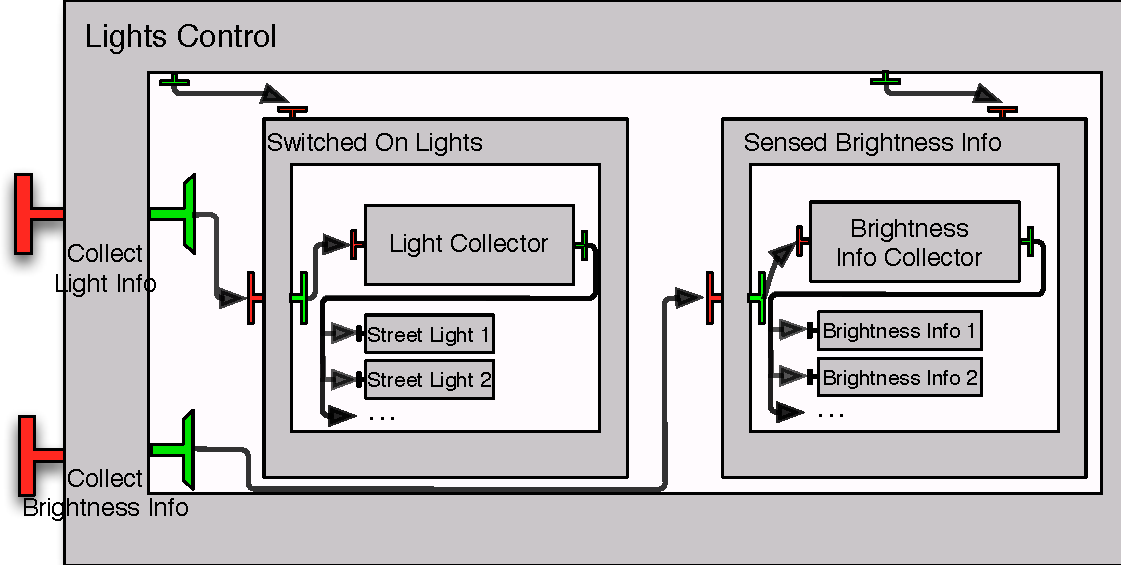
\includegraphics[scale=0.5]{figures/chapter4/usecasearch.pdf} 
   		\caption{Use-Case Architecture}
   		\label{fig:auto}
		\end{figure}

\noindent This use-case consists in an experimental \textsf{component} system 
  in charge of switching on and off street lights, according to the perceived 
  luminosity of the surroundings. Basically, in order to address the goal of
  saving energy, but at the same time offering an acceptable quality of service
  (i.e. an acceptable luminosity in the streets), the \textsf{component}s \textit{Street Light}
  and \textit{Brightness Info} are added/removed accordingly. Moreover, as
 said in \cite{BHN:ICAS09}, the use-case starts with three \textit{Brightness Info}
 \textsf{component}s and zero \textit{Street Light} \textsf{component}. 
  
 We model this scenario in \textsc{Mefresa} by defining every
 \textsf{component} involved in the architecture. For instance, \textsf{component}s
 \textit{Light Collector} and \textit{Street Light} are mechanized as follows:
  
\lstinputlisting[language=Coq]{listings/chapter4/usecase.tex}	
  
  
  \noindent In the above definitions, \textbf{p1} holds the path of 
  both \textsf{component}s in the hierarchy.
  Furthermore, the remaining \textsf{component}s are defined in a similar 
  fashion.  Considering the
  variable \textsf{LightsControlUseCaseArchitecture} as the
  structure holding the complete hierarchy, we can prove its
  well-formedness.
  
\lstinputlisting[language=Coq]{listings/chapter4/usecasearch.tex}	  
  
	\noindent The architecture from this use case indeed meets
	the specification, and proving this lemma poses no particular challenge
	as it has an explicit structure. The interesting aspect of this use-case
	comes from the fact that we need to add and remove \textsf{component}s at runtime.
	Indeed, this scenario is yet another example of the usefulness of being able to
    cope with parametrized specifications.     
    
    
  Before proceeding to the structural reconfigurations, we 
  shall use our \textit{operation} language 
  constructs to define new,
  higher-level constructs. For instance, we can easily define an \textsf{operation}
  to build several \textsf{component}s at a time:
  
  \lstinputlisting[language=Coq]{listings/chapter4/mkcomponents.tex}		
 
\noindent This new \textsf{operation} \textsf{mk\_components} takes
a list of \textsf{component}s as argument and produces a sequence of
\textsf{mk\_component} \textsf{operation}s by means of our 
\textbf{;} constructor. Further, we shall also define an \textsf{operation}
for the construction of a list of \textsf{binding}s.
 
 \lstinputlisting[language=Coq]{listings/chapter4/mkmulticast.tex}

\noindent %As mentioned above, there are three types of bindings -
%\textit{normal}, \textit{import} and \textit{export} -,
%therefore it is natural to imagine three types of multicasts. 

Essentially, it is 
a set of \textsf{binding}s being made from the same client to several
servers. The path \textbf{p} is given as pointer to the \textsf{component} in the hierarchy
where the \textsf{binding} is going to be kept. Then,  we specify the identifiers \textbf{icc}
and \textbf{iic} that determine the \textsf{component} and \textsf{interface} from which the
\textsf{binding} is made from. Since each \textsf{binding} is made to a different \textsf{component},
we need to generate different identifiers. This is achieved in the same manner
as with the \textsf{generate\_from\_template} function defined above: at each
recursion step we suffix \textbf{n} to \textbf{ics} so that we target different \textsf{component}s
for every \textsf{binding} built. Finally, the identifier \textbf{iis} gives the \textsf{interface} to 
which the \textsf{binding} is made to.
 
Having defined our new \textsf{operation}s, we can now proceed to the specification
of the reconfiguration to add \textit{"Street Light"} \textsf{component}s. Below, \textsf{LightComp}
is a variable representing our \textit{"Street Light"} \textsf{component} defined above.
 
\lstinputlisting[language=Coq]{listings/chapter4/usecasereconfig.tex}
 
\noindent Basically, the above creates \textbf{n} \textsf{component}s
by using the \textit{"Street Light"} \textsf{component} as template, and 
then establishes the required \textsf{binding}s. This, could for instance be
used as follows:

\lstinputlisting[language=Coq]{listings/chapter4/usecaseproof.tex}

\noindent Proving the above lemmas is achieved by the same reasoning
techniques as discussed above. Regarding the first lemma, the key ingredient here to note is that
\textsf{component}s are created before establishing the \textsf{binding}s --- and thus
\textsf{binding}s will indeed succeed to be established --- and they are well-formed
since they are generated from a well-formed template \textsf{component}. As such,
reducing this \textsf{operation} to \textbf{Done} is possible. It should be noted that while generalizing
this lemma for \textbf{n} would require a proof by induction, it would still follow the same principle.
As for the second lemma,
it is a natural consequence of our \textit{validity} theorem (see Listing \ref{lst:validity}).



%% @@@@@@@@@@@@
\section{Discussion}
\label{sec:mesfresadiscussion}


	In this chapter we presented a framework to reason
	about the structure of \textsf{GCM} applications mechanized in the Coq Proof Assistant. 
    The main novelty of our approach lies in the use of an \textsf{operation} language
    that allows to build software architectures	that are \textit{correct-by-construction}.
    While we lose some of the automation offered by the usual approach followed by the use of 
	model-checkers, relying on the expressiveness of the Coq Proof Assistant allows us
	to reason on issues that cannot be addressed by usual model-checking techniques.	
	
	The choice of a \textit{deep-embedding} rather than a \textit{shallow} 
	approach for the definition of our  \textsf{operation} language	is also worth discussing.	
	By explicitly using a \textit{datatype} for the encoding of our \textsf{operation} language 
	there is a clear identification of its syntax, letting no doubt on how \textsf{operations} can
	be composed. Further, our goal here is also to formalize the \ac{GCM} specification, a \textit{deep-embedding}
	emphasizes the operational semantics for the building and reconfiguration of architectures. 
		
%	interesting challenges w.r.t. distributed component-based applications structure.
	
	Indeed, the definition of the \ac{GCM} specification in natural language opens
	the door for several interpretations. Further, such a specification is supposed
	to be \textit{flexible} and allow various conceivable implementations. 
	Nevertheless, the \textsc{Mefresa} framework shows that it is possible and fruitful
	to formalize such an undertaking in a proof assistant like Coq.
	Further, is also provides a case-study on the mechanization of \textsf{component} models in
	the context of interactive theorem proving. In fact, the need for such an approach was
	already discussed in \cite{MERLE:2008:INRIA-00338987:1}.
	
	
	%in the Coq Proof Assistant. Our approach differs from the remaining in that we 
	%aim at 
	%providing a semantics that allows the building of  \textit{correct-by-construction} architectures.

	%\paragraph{}
	%adl is the starting point


	%\paragraph{}
	%complementary approach




\chapbreak

	In this chapter we presented \textsc{Mefresa}, a Coq framework for the reasoning on software architectures.
	
		In the following Chapter we show its practical facet by demonstrating how we integrated it		
		with the ProActive middleware, and the inherent benefits from this combination.



 %Mefresa
       % Chapter 5

\chapter{\textsf{Painless} integration with ProActive} 
\label{chap:extraction} 


\epigraph{\textit{“Many will call me an adventurer - and that I am, only one of a different sort: 
                             one of those who risks his skin to prove his platitudes."}}{Che Guevara}



\minitoc

\lhead{Chapter 1. \emph{\textsf{Painless} integration with ProActive}} % This is for the header on each page - perhaps a shortened title

%----------------------------------------------------------------------------------------

\section{Extracting a certified \textsf{Painless} interpreter}
\label{sec:extraction}

\subsection{Certified functional code from logical specifications}
\label{sub:execcode}
%mencionar paper que loulerge me falou

\subsection{The remaining bits: adjusting to OCaml native types}
\label{sub:ocamltypes}



\section{\textsf{Painless} support for the static and runtime verification of GCM/ProActive Applications}
\label{sec:prointegration}

%\subsection{Integration with Ocaml-Java}
%\label{sub:}


\section{Architectural classes for statically ensuring safe reconfigurations} %without runtime checks
\label{sec:noruntime}


\section{Discussion}
\label{sec:discussion}

 % Painless
        % Chapter 7

\chapter{Mechanized behavioural semantics} 
\label{chap:behaviour} 

\epigraph{\textit{“Yet, ..."}}{Nuno Gaspar}



\minitoc


\lhead{Chapter 7. \emph{Mechanized behavioural semantics}} % This is for the header on each page - perhaps a shortened title

%----------------------------------------------------------------------------------------

	This chapter discusses the mechanization, in the Coq proof assistant, of a behavioural 
semantics based on the execution trace of synchronized labelled transition systems. Further, we show
how it can be used in the context of \ac{GCM} applications.

	Section \ref{sec:pLTS} presents the mechanization of \ac{LTS} and
their traces. We show how we can synchronize several \ac{LTS} in Section \ref{sec:pnet}.
Then, we exemplify its use in the context of \ac{GCM} applications in Section \ref{sec:gcmpnets}.
For last, Section \ref{sec:behaviourdiscussion} discusses the final remarks about this
mechanization.


\section{Labelled transition systems, and traces}
\label{sec:pLTS}

	
	\lstinputlisting[language=Coq, stepnumber=1, 
	                      caption={\textsf{lts\_state} datatype}, 
	                      %firstnumber=19,
	                      label=lst:ltsstate]{listings/chapter6/state.tex}	
	
	
	\noindent A \textsf{lts\_state} is identified by a natural number, and holds an internal memory that is a
	simple mapping between strings to naturals. For the sake of simplicity we directly use strings to denote variables,
	and constrain ourselves to natural number values.
	
	Next, let us now see the \textsf{action} datatype. Listing \ref{lst:action} illustrates its definition.
	
		\lstinputlisting[language=Coq, stepnumber=1, 
	                      caption={\textsf{action} datatype}, 
	                      %firstnumber=19,
	                      label=lst:action]{listings/chapter6/action.tex}	

	\noindent An \textsf{action} is composed by a \textsf{message}, and a set of \textsf{assignments}.
	As expected, the latter permits to specify the assignment of specific state variables to a \textsf{transition}.
	The former holds the label, its type of communication and a set of parameters. Listing \ref{lst:message}
	depicts its definition.
	
			\lstinputlisting[language=Coq, stepnumber=1, 
	                      caption={\textsf{message} datatype}, 
	                      %firstnumber=19,
	                      label=lst:message]{listings/chapter6/message.tex}	

	\noindent A message can either be \textit{reading} or \textit{emitting} (lines 2-3). Typically, these
	are used to receive and transmit values, respectively. Naturally, the allowed \textsf{parameters} are
	either values --- natural numbers --- or variables (lines 6-7).
	
	
	Finally, we can now see the \textsf{LTS} datatype as depicted by Listing \ref{lst:lts}.	
		
	\lstinputlisting[language=Coq, stepnumber=1, 
	                      caption={\textsf{LTS} datatype}, 
	                      %firstnumber=19,
	                      label=lst:lts]{listings/chapter6/LTS.tex}	

	Having defined the \textsf{LTS} datatype, we can now define \textsf{traces}. A trace is a sequence of actions 
	resulting from the sequence of \textsf{transitions} taken by the \textsf{LTS}. It can either be finite or
	infinite. A finite trace means that a \textit{sink} state was attained, thus the execution \textit{deadlocks}.
	Listing \ref{lst:ltstrace} defines a \textsf{LTS} trace.	
	
	
		\lstinputlisting[language=Coq, stepnumber=1, 
	                      caption={Trace definition for a \textsf{LTS}}, 
	                      %firstnumber=19,
	                      label=lst:ltstrace]{listings/chapter6/ltstrace.tex}	


	\noindent A \textsf{LTS\_Trace} is defined by a co-inductive predicate since we potentially deal
	with infinite sequences. The expression, \textsf{LTS\_Trace A q l}, means that \textsf{l} is a trace
	in the \textsf{LTS} object \textsf{A}, starting from the state \textsf{q}.   

		The \textsf{LTS\_Trace} predicate is composed by two constructors: \textsf{lts\_empty\_trace} (line 2)
	and \textsf{lts\_cons\_trace} (line 8).  The former simply expresses that, from any state, 
	all \textsf{actions} of the \textsf{LTS} yield no target state (lines 3-5). Indeed, the
	function 
	\textsf{lts\_target\_state : LTS $\rightarrow$ lts\_state $\rightarrow$ message $\rightarrow$ lts\_state}
	is responsible for computing the attained state from \textsf{q} with an \textsf{action} holding the message
	\textsf{m}. Thus, the constructor's conclusion is \textsf{LTS\_Trace A q LNil}, since the trace from \textsf{q}
	is empty.	The latter constructor however, demands the that we reach a state \textsf{q'} (line 11), and
	a trace from \textsf{q'} (line 12), in order to conclude \textsf{LTS\_Trace A q (LCons (Action m asgns) l)} (line 13).
	
		For the sake of clarity, Listing \ref{lst:ltstargetstate} depicts the \textsf{lts\_target\_state} function.	
	
		\lstinputlisting[language=Coq, stepnumber=1, 
	                      caption={\textsf{lts\_target\_state} function definition}, 
	                      %firstnumber=19,
	                      label=lst:ltstargetstate]{listings/chapter6/ltstargetstate.tex}			
	
	
	\noindent The function pattern matches the \textsf{message m} and checks whether its label
	is equal to \textsf{"-"}. If it is the case then it simply returns the current state \textsf{st} (line 19),
	otherwise it proceeds by calling the \textsf{lts\_get\_target\_state} function (line 20).
	The is due to the fact that we consider a \textsf{message} with a \textsf{"-"} label as
	a special case. As we shall see in Section \ref{sec:pnet}, this exception is related with the 
	way we deal with synchronization between \ac{LTS}.
	
	The \textsf{lts\_get\_target\_state} function starts by pattern matching on the \textsf{LTS}
	list of \textsf{transitions} (line 3),  returning no state if its empty (line 4). If it is not the 
	case (line 5), then we check if the \textsf{transition} at the head of the list possesses
	a source state that matches the parameter state \textsf{st}, and if the \textsf{message} contained
	in its \textsf{action} is equal to the parameter \textsf{message m} (line 6). Should that be the case,
	then it simply process the assignments associated with the taken \textsf{action} (line 9), and updates
	the target state memory accordingly (line 10). As expected, this the the purpose of the
	\textsf{process\_assignment : state\_mem $\rightarrow$ assignments $\rightarrow$ state\_mem} function, 
	and \textsf{-$>>$} notation, respectively. Otherwise it recurs on the tail of the list of 
	\textsf{transitions} (line 13).

	



\section{Synchronization of LTS, and traces}
\label{sec:pnet}

	In the previous Section we saw how to model a single \ac{LTS}. However, it is often the case
	that we want to be able to have several \ac{LTS} communicate with each other.	This is achieved
	by synchronizing their \textsf{actions}.
	
		First, let us formalize the notion of a synchronization vector. Listing \ref{lst:synchvectors}
	depicts its datatype.	
	
	\lstinputlisting[language=Coq, stepnumber=1, 
                      caption={\textsf{SynchronizationVector} datatype}, 
                      %firstnumber=19,
                      label=lst:synchvectors]{listings/chapter6/synchvectors.tex}		

	\noindent Basically, a synchronization vector is composed by a list of synchronization elements,
	and an output element (line 9). The former indicate the \textsf{actions} that need to be considered among
	the list of \ac{LTS} being synchronized. The latter stands for the resulting global action.  
	Both synchronization and output elements are represented by string values. For the sake of convenience
	we also permit synchronization elements to be defined through the \textsf{WildCard} constructor (line 2).
	Further we define a notation as depicted by Listing \ref{lst:synchvectorsnotation}.
	
	\lstinputlisting[language=Coq, stepnumber=1, 
                      caption={A convenient notation for \textsf{SynchronizationVector}}, 
                      %firstnumber=19,
                      label=lst:synchvectorsnotation]{listings/chapter6/synchvectorsnotation.tex}	
                      	
    \noindent Basically, it permits Coq to directly understand expressions such 
    as the following one: \textsf{$<<$ "x" , "y" , "-" , "z" $>>$ -> "XYZ"}.

	Let us now define a type for a communicating network of \ac{LTS}. We shall call this type \textsf{Net}.
	Its definition is depicted by Listing \ref{lst:net}.	

	\lstinputlisting[language=Coq, stepnumber=1, 
                     caption={\textsf{Net} datatype}, 
                     %firstnumber=19,
                     label=lst:net]{listings/chapter6/net.tex}	

	\noindent It is composed by two constructors: \textsf{mk\_SingletonNet} and \textsf{mk\_Net}.
	The former is used for simple models constituted with a single \ac{LTS}, while the latter
	permits to specify communicating \ac{LTS} by means of synchronization vectors.
	
	For this new structure we need a new notion of state. Listing \ref{lst:netstate} depicts the \textsf{pnet\_state}
	datatype.

	\lstinputlisting[language=Coq, stepnumber=1, 
                     caption={\textsf{net\_state} datatype}, 
                     %firstnumber=19,
                     label=lst:netstate]{listings/chapter6/netstate.tex}	

	\noindent Basically, both its constructors follow the same rationale: they keep track of the 
	involved \textsf{lst\_states}. 
	
	%indexed_membership
	%attainable
	
	Before proceeding to the definition of traces for	\textsf{Net}s, we need to consider
	how their transitions are performed. For this case, we need to consider the current
	\textsf{net\_state} and the activated synchronization vector. Moreover, each synchronization
	element may permit more than one \textsf{action} to occur. Thus, a function
	computing the target \textsf{net\_state}s must also return the resulting global action.
	Listing \ref{lst:nettargetstates} depicts such a function.
		
	\lstinputlisting[language=Coqfix, stepnumber=1, 
                     caption={\textsf{net\_target\_states} function definition}, 
                     %firstnumber=19,
                     label=lst:nettargetstates]{listings/chapter6/nettargetstates.tex}		
	
	
	\noindent The above function may seem complicated at first sight, and requires 
	a closer look. Basically, it starts by pattern matching on its \textsf{Net} parameter
	\textsf{net\_obj}, \textsf{net\_state} parameter \textsf{q}, and synchronization vector parameter
	\textsf{sv} (line 3). The function is supposed to be used with \textsf{Net} objects and \textsf{net\_state}
	modelling systems with \textsf{LTS} synchronization. Should that not be the case, it simply returns
	an empty list (line 17).
	
		
		Another useful function concerns the computation of the initial state of a \textsf{Net}.
	Listing \ref{lst:initnet} depicts its definition.
	
	\lstinputlisting[language=Coqfix, stepnumber=1, 
                     caption={\textsf{init\_net\_state} function}, 
                     %firstnumber=19,
                     label=lst:initnet]{listings/chapter6/initnet.tex}		
	
	\noindent Basically, the above function computes the initial state of a \textsf{Net}. This is achieved
	by pattern matching on the \textsf{Net} parameter \textsf{net\_obj} (line 2). If it is
	a \textsf{Net} with a single \textsf{LTS} object, than it simply returns the adequate \textsf{net\_state}
	constructor with the initial state of the \textsf{LTS} (line 3). Otherwise, it recursively
	gathers the initial state of each \textsf{LTS} objects composing \textsf{net\_obj} into
	the local variable \textsf{lq} (lines 5-9), and returns the adequate \textsf{net\_state}
	constructor with \textsf{lq} (line 10).
	
				
	
	
	
		
	
	
	
	Let us now define a predicate indicating whether a state can attain another state. Listing \ref{lst:attainable}
	depicts its formalization.
			
			\lstinputlisting[language=Coq, stepnumber=1, 
                     caption={\textsf{attainable} predicate definition}, 
                     %firstnumber=19,
                     label=lst:attainable]{listings/chapter6/attainable.tex}	
	
		
	\noindent 
	
	
	
		As expected, traces for \textsf{Net}s are slightly more involved than traces for \textsc{LTS}. 
	Listing \ref{lst:nettrace} formalizes the notion of trace for the \textsf{Net} datatype.
			

		\lstinputlisting[language=Coq, stepnumber=1, 
                     caption={Trace definition for \textsf{Net}}, 
                     %firstnumber=19,
                     label=lst:nettrace]{listings/chapter6/nettrace.tex}	
	
	\noindent It is composed by three constructors: \textsf{lts\_trace},
	\textsf{net\_empty\_trace} and \textsf{net\_lcons\_trace}.
		
	
	


\section{Modelling GCM internals}
\label{sec:gcmpnets}



\section{Discussion}
\label{sec:behaviourdiscussion}


	


\chapbreak

	In this chapter we presented the mechanization of a behavioural 
semantics based on the execution trace of synchronized labelled transition systems. Further, we
exemplified its use in the context of \ac{GCM} applications.
	
	In the following chapter we discuss the works related with this thesis.



 % Painless
        % Chapter 6

\chapter{Related Work} 
\label{chap:related} 


\epigraph{\textit{“If you know the enemy and know yourself you need 
                             not fear the results of a hundred battles."}}{Sun Tzu}

\minitoc

\lhead{Chapter 6. \emph{Related Work}} % This is for the header on each page - perhaps a shortened title

%----------------------------------------------------------------------------------------

\section{On the HyperManager use case}
\label{sec:relhyper}

	%byzantine fault : disse que queria reconfig.
	%use case cadp site...
	%BIP framework? ou na secao mefresa?

	\cite{BHHM:FACS11} madelaine case study
	
	
	Compositional Verification for Component-Based Systems and Application
	http://www-verimag.imag.fr/~sifakis/atva2008.pdf
	\cite{BBN+10} 


	FACS:
	  The maturity attained by the CADP toolbox 
		made it a reference tool among the formal methods community.  Several case studies have been published, 
		namely industrial ones addressing other goals than verification. For instance, in \cite{conf/cav/CosteHLS09}
	Coste et. al. discuss performance evaluation for systems and networks on chips.			
	 More closely related with our work we must refer the experiments presented in 
	 \cite{conf/dais/CornejoGMP01}. A dynamic reconfiguration protocol is specified and model-checked,
	 however their focus is on the reconfiguration protocol itself rather than reconfigurable applications.
		 
		  	
		Indeed, many works can be found in the literature embracing a behavioural semantics
		approach for the specification and verification of distributed systems. Yet, 
		literature addressing the aspects of reconfigurable applications remains 
		scarce. 

		
 Nevertheless, we must cite the work around
	    %BIP
	    BIP (Behaviour, Interaction, Priority) \cite{BBB+11a} --- a framework 
	 encompassing rigorous design principles. It allows the description of the 
	 coordination between components
	 in a layered way. Moreover, it has the particularity of also permitting the 
	 generation of code from its models. Yet, structural reconfigurations are not supported. 
	 	
	%CHARMY	
	Another rather different approach that we must refer is the one followed by tools 
	specifically tailored for architectural specifications. For instance, in \cite{p.2005-1} Inverardi et. al. 
	discusses \textsf{CHARMY}, a framework for designing and validating architectural 
	specifications. It offers a full featured graphical interface with the goal of being more 
	\textit{user friendly} in an industrial context. Still,
	architectural specifications remain of static nature. 
	
	
	
		Looking at the interactive theorem proving arena we can also find some
	related material. In %coq stuff
	\cite{Boyer:2013:RRC:2486788.2486791} Boyer et. al. propose a reconfiguration protocol
	and prove its correctness in the Coq Proof Assistant \cite{09thecoq}. This work however, focuses on the protocol itself, 
	and not in the behaviour of a reconfigurable application. 
   





\section{On the Mefresa framework}
\label{sec:relmefresa}


%creol

	%    henrio.
 %   Nev- ertheless, we must cite the work from Henrio et al. [12] on a framework for reasoning on the behaviour of GCM component composition mechanized in Isabelle/HOL [18]. Our approach is still considerably different in that we pro- vide a semantics for an operation language for the building and reconfiguration of GCM architectures.
 
 Many approaches regarding the formalization of component models can be found in the literature. Yet,
	to the best of our knowledge this is the first work aiming at providing a mechanized framework
    that applies the \textit{correct-by-construction} paradigm to the world of component-based engineering.
	Nevertheless, we must cite the work from Henrio et al. \cite{HKK:FMCO09} on a framework for reasoning 
	on the behaviour of GCM component composition mechanized in Isabelle/HOL \cite{Nipkow-Paulson-Wenzel:2002}. 
	Our approach is still considerably different
	in that we provide a semantics for an \textit{operation} language for the building 
	and reconfiguration of GCM architectures.
	
	%work of Coq from INRIA Sardes	: http://perso.ens-lyon.fr/damien.pous/rrca/ http://2013.icse-conferences.org/
	
	
	%CREOL
	Another work involving the use of a proof assistant is the work by Johnsen et. al. 
	on the \textsf{Creol} framework \cite{johnsen06tcs}. \textsf{Creol} focuses on
	the reasoning of distributed systems by providing a high-level object oriented
	modelling language. Its operational semantics are defined in the rewriting logic tool 
	Maude \cite{Maude2:03}. This work however does not contemplate architectural 
	reconfigurations and follows a methodology in the style of a Hoare Logic. 	
		
    

   	
	%most stuff is "just" model checking
	%invited speaker conf. http://www.di.univaq.it/inverard/
	%http://www.di.univaq.it/charmy/
	Indeed, while the use of proof assistants is gaining notoriety, model-checking is still
	the \textit{de facto} formal approach for both industrial and academic undertakings.
	Usually, some form of state machine model is used for the design of the intended
	system,  and then a carefully chosen model-checker as back-end is employed as
	a decision procedure. %This is for instance the methology followed in our Vercors
	%platform \cite{Barros:2007:MDC:1269985.1270075}. 
	For instance, in \cite{p.2005-1} Inverardi et. al. 
	discusses \textsf{CHARMY}, a framework for designing and validating architectural 
	specifications. It offers a full featured graphical interface with the goal of being more 
	\textit{user friendly} in an industrial scenario. Still,
	architectural specifications remain of static nature. 
	The BIP (Behaviour, Interaction, Priority) 
	framework \cite{BBB+11a} formalizes and specifies component interactions.
	It has the particularity of also permitting the generation of code from its models.
	

	%formal spec alloy  -> they recommend Coq
   	Moreover, a formal specification of the Fractal Component Model has 
   	been proposed in the  Alloy specification language \cite{MERLE:2008:INRIA-00338987:1}. 
	This work proves the consistency of a (set-theoretic) model of Fractal applications. 	 
	Their goal was to clarify the inherent ambiguities of the informal specification presented
  	in \cite{fractalSpec}. Their specification however, is constrained by the first-order relational logic nature 
   	of the Alloy Analyzer. In fact, they point to the use of the Coq Proof Assistant in order 
   	to overcome this limitation.	
	
	
	%era PC ano passado
	%Let us also mention previous work by Aldrich on the use of a type system at the source code level to 
	%enforce architectural constraints \cite{Aldrich:2008:UTE:1343599.1344114}. This is a rather different
	%approach than ours as it is a direct extension of the Java programming language with type annotations
	%that are statically checked. Allowing for flexible and dynamic designs is within the goals of the project,	
	%but structural reconfigurations are not supported.


	%\paragraph{}
	%see JNO 

	%in the spirit of dynamic ADLs
	%\paragraph{}
	%may want to refer dynamic ADLs ?

	%fpath &fscript
	For last, from a more engineering point of view, we can refer the work around FPath and FScript \cite{journals/adt/DavidLLC09}.
	FPath is a domain-specific language for the navigation and querying of Fractal architectures. FScript embeds the FPath
	language and acts as a scripting language for the specification of reconfigurations strategies. The main goal of this
	work however is to alleviate the need to interact with the low-level API. Further, reliability of these reconfigurations
	is ensured by run-time checking, while we are more concerned on providing guarantees statically.
	
	%\paragraph{}
	%Extension to previous work \cite{gaspar:hal-00725291}


\section{On Painless}
\label{sec:relpainless}

	Several proposals for \ac{ADL}s can be found in the literature, each with their own 
	particularities and attempting to 
	address their specific application domain concerns. 
	
	%http://www-systems.cs.st-andrews.ac.uk/wiki/ArchWare/
	The work around the ArchWare \ac{ADL} \cite{DBLP:journals/corr/abs-1006-4829} 
	is of particular interest. They claim that 
	\textit{"software that cannot change is condemned to atrophy"}	
	and introduce the concept of an \textit{active software architecture} in order
	to address this challenge. Based on the higher-order $\pi$-calculus, it provides
	constructs for specifying control flow, communication and dynamic topology.
	Unlike \textsc{Painless}, its syntax exhibits an imperative style 
	and type inference is not supported, thus not promoting concise specifications. 
	
	Nevertheless, it is sufficiently rich to provide executable specifications of active software
	architectures. Moreover, user-defined constraints are supported through the ArchWare 
	Architecture Analysis Language. Yet, their focus is more aimed at the specification
	and analysis of the \ac{ADL}, rather than actual application execution and deployment.
	In our work, the user solely defines the architecture of its application, structural constraints
	are implicit: they are within the mechanized \ac{GCM} specification.	Further, our tool support
	is tightly coupled with the ProActive middleware.
	
		
	%ref Archery
		Also from the realm of process algebras, Archery \cite{conf/facs2/SanchezBR11} is a modelling
	language for software architectural patterns. It is composed by a core language and two extensions:
	\textsf{Archery-Core}, \textsf{Archery-Script} and \textsf{Archery-Structural-Constraint}.
	These permit the specification of structural and behavioural dimensions of architectures,
	the definition of scripts for  reconfiguration, and the formulation of structural constraints,
	respectively. Moreover, a bigraphical semantics is defined for Archery specifications. This grants
	the reduction of the constraint satisfaction verification to a type-checking problem. However,
	this process is not guarantee to be automatic, and type-checking decidability remains as future work.
	
	
	%%check refs....
	%falta darwin..
				
		
	%logic based. http://ce-resd.facom.ufms.br/sbrc/1994/p10.pdf
	As expected, logic is also a natural formalism of choice. For instance, Gerel \cite{endler1992}
	is a generic reconfiguration language including powerful query constructs based on first-order logic.
	Further, its reconfiguration procedures may contain preconditions \textit{\`a la} 
	Hoare Logic \cite{Hoare69anaxiomatic}. These are evaluated by brute force. It is unclear
	how they cope with the inherent undecidability of such task. 
	%paper runtime verif. http://hal.archives-ouvertes.fr/docs/00/64/23/45/PDF/facs2011_preproceedings_9.pdf
	%favs 2011
	%temporal logic to FScript ... undecidable problem in conclusion...


		%graph based:
	Furthermore, the use of a graph-based formalism for the specification of software architectures
	is also rather popular. For instance, in \cite{Bruni:2008:GDA:1424922.1424928} two graph-based
	approaches and related tool support are compared. Another interesting aspect of this work
	regards the use of the Alloy Analyzer \cite{Jackson:2002:ALO:505145.505149}, 
	and Maude \cite{Clavel:2002:MSP:633559.633563} as a means to show the approaches' feasibility. 
		

		More recently, 	Di Cosmo et. al. defined the Aeolus component model \cite{conf/sefm/CosmoZZ12}. Their focus
	is on the automation of cloud-based applications deployment scenarios. Nevertheless, their 
    proposal is still loosely inspired by the Fractal component model \cite{fractalSpec} whose
	most peculiar characteristics are its hierarchical composition nature and reconfiguration capabilities.
	However, while both approaches permit architectural reconfigurations at runtime, 
    its specification is not supported by their ADL, it solely contemplates deployment related
    aspects. Moreover, support for
	parametrized specifications is also not covered, forcing the software architect to explicitly 	
	define the application's structure.    
	
		Regarding Fractal,  it is also worth noticing that they try to overcome the lack of
	support for reconfiguration specification	 through 
	Fscript \cite{DAVID:2008:HAL-00468474:1}. Fscript embeds FPath --- a DSL for navigation and querying of
	Fractal architectures --- and acts as a scripting language for reconfiguration strategies. These
	are not evaluated for their validity. Nevertheless, system consistency is ensured by the use of
	\textit{transactions}: a violating reconfiguration is \textit{rolled back}.
	Furthermore, an interesting feature is the support for application-specific architectural
	invariants.


	%ref survey 2/5
	%	scalability / types.. logic etc
	%question "Given system x, what happens when change y occurs?"
	%para tese devo colocar me em todas as tabelas referidas..
		To conclude, let us mention a survey regarding the approaches for the specification of 
	dynamic software architectures \cite{Bradbury:2004:SSD:1075405.1075411}. These are 
	classified into four categories: graph-based, process algebra-based, 
	logic-based, and other. To this end, we place ourselves
	in the \textit{other} category. Indeed, while formal logic is at the foundation of 
	our approach, all the machinery involving requirement/constraint checking is 
	implicit and done automatically by our Coq development. The software architect 
	solely uses a language with a declarative trait. %Another important factor referred by 
	%this survey concerns scalability. In general, a decentralized or distributed approach
	%is more likely to scale. This is the case for \textsc{Painless}, as	
	
	
	
		
	
		
	
	
	
	 %oleksandra
    
    
    %Indeed, its structural information remains of static nature, therefore 
	%not revealing the full picture regarding an application topology. 	





 %related work
         % Chapter 7

\chapter{Final Remarks} 
\label{chap:conclusion} 

\epigraph{\textit{“Yet, ..."}}{Nuno Gaspar}



\minitoc


\lhead{Chapter 1. \emph{Final Remarks}} % This is for the header on each page - perhaps a shortened title

%----------------------------------------------------------------------------------------






%final

   % \appendix
   % \chapter{Appendix 1} % (fold)
\label{cha:app1}




    \backmatter
    %%\cleardoublepage
%\bibliographystyle{alpha}
%\refstepcounter{chapter}
%\addcontentsline{toc}{chapter}{\bibname}
%\bibliography{thesis}
\printbibliography
\adjustmtc

    \bibliographystyle{IEEEtran}
    \nocite{*}
    \bibliography{thesis}
    \chapter{List of Acronyms} % (fold)
\label{cha:listofacronyms}

\begin{acronym}[AAAAAA]
    \acro{ADL}{Architecture Description Language}
    \acro{GCM}{Grid Component Model}
    \acro{API}{Application Programming Interface}
    \acro{FIFO}{First In, First Out}
    \acro{ECW}{E-Connectware}
    \acro{LTS}{Labelled Transition System}
    \acro{LTL}{Linear Temporal Logic}
    \acro{SVL}{Script Verification Language}
    \acro{MCL}{Model Checking Language}
    \acro{RFID}{Radio-Frequency Identification}
    \acro{JMX}{Java Management Extensions}
\end{acronym}

% chapter list_of_acronyms (end)

\end{document}
